\documentclass[11pt,a4paper]{article}
\usepackage[margin=2.3cm]{geometry}
\usepackage[T1]{fontenc}
\usepackage[sc]{mathpazo}
\usepackage[scaled=0.92]{helvet}
\usepackage{courier}
\usepackage[section]{placeins}
\linespread{1.05}
\usepackage{amsmath,amssymb}
\usepackage{booktabs,longtable,array}
\usepackage{graphicx}
\usepackage[font=small,labelfont=bf,margin=0pt]{caption}
\usepackage{xcolor}
\usepackage{enumitem}
\usepackage{microtype}
\usepackage{algorithm}
\usepackage[noend]{algpseudocode}
\usepackage[round,authoryear]{natbib}
\usepackage[colorlinks=true,linkcolor={blue!45!black},citecolor={blue!45!black},urlcolor={blue!45!black}]{hyperref}
\hypersetup{pdftitle={Terrain dependence of heart-rate-based VO2max estimation: mechanisms, a within-runner field test on 9962 runs, and a terrain-robust estimator},pdfauthor={Jos\'e A. Garc\'ia and Rosa Rodriguez-S\'anchez}}
\setlist{itemsep=2pt,topsep=4pt}
\setlength{\emergencystretch}{1.5em}
% generated by make_tables.py
\newcommand{\nablBFreeHmountain}{\ensuremath{-}0.20}
\newcommand{\nablBFreeHroadflat}{\ensuremath{-}0.31}
\newcommand{\nablBFreeHskyrun}{\ensuremath{-}0.53}
\newcommand{\nablBFreeHtrailrunnable}{\ensuremath{-}0.01}
\newcommand{\nablBFullmountain}{\ensuremath{-}2.01}
\newcommand{\nablBFullroadflat}{\ensuremath{-}0.32}
\newcommand{\nablBFullskyrun}{\ensuremath{-}1.44}
\newcommand{\nablBFulltrailrunnable}{\ensuremath{-}0.57}
\newcommand{\nablBNoAltmountain}{\ensuremath{-}4.37}
\newcommand{\nablBNoAltroadflat}{\ensuremath{-}1.47}
\newcommand{\nablBNoAltskyrun}{\ensuremath{-}5.56}
\newcommand{\nablBNoAlttrailrunnable}{\ensuremath{-}1.49}
\newcommand{\nablBNoDescmountain}{\ensuremath{-}3.40}
\newcommand{\nablBNoDescroadflat}{\ensuremath{-}0.45}
\newcommand{\nablBNoDescskyrun}{\ensuremath{+}2.42}
\newcommand{\nablBNoDesctrailrunnable}{\ensuremath{-}1.33}
\newcommand{\nablBNoDriftmountain}{\ensuremath{-}3.97}
\newcommand{\nablBNoDriftroadflat}{\ensuremath{-}1.60}
\newcommand{\nablBNoDriftskyrun}{\ensuremath{-}5.12}
\newcommand{\nablBNoDrifttrailrunnable}{\ensuremath{-}2.38}
\newcommand{\nablBNoGaitmountain}{\ensuremath{-}0.51}
\newcommand{\nablBNoGaitroadflat}{\ensuremath{-}0.30}
\newcommand{\nablBNoGaitskyrun}{\ensuremath{+}3.36}
\newcommand{\nablBNoGaittrailrunnable}{\ensuremath{-}0.55}
\newcommand{\nablBNoLagmountain}{\ensuremath{-}1.18}
\newcommand{\nablBNoLagroadflat}{\ensuremath{+}0.20}
\newcommand{\nablBNoLagskyrun}{\ensuremath{-}0.66}
\newcommand{\nablBNoLagtrailrunnable}{\ensuremath{+}0.08}
\newcommand{\nablBNoWmountain}{\ensuremath{-}2.75}
\newcommand{\nablBNoWroadflat}{\ensuremath{-}0.34}
\newcommand{\nablBNoWskyrun}{\ensuremath{+}0.35}
\newcommand{\nablBNoWtrailrunnable}{\ensuremath{-}0.68}
\newcommand{\nablFreeHmountain}{3.19}
\newcommand{\nablFreeHroadflat}{0.71}
\newcommand{\nablFreeHskyrun}{4.05}
\newcommand{\nablFreeHtrailrunnable}{2.76}
\newcommand{\nablFullmountain}{2.93}
\newcommand{\nablFullroadflat}{0.74}
\newcommand{\nablFullskyrun}{3.10}
\newcommand{\nablFulltrailrunnable}{1.52}
\newcommand{\nablMBFreeHmountain}{\ensuremath{+}0.02}
\newcommand{\nablMBFreeHroadflat}{\ensuremath{-}0.12}
\newcommand{\nablMBFreeHskyrun}{\ensuremath{+}0.13}
\newcommand{\nablMBFreeHtrailrunnable}{\ensuremath{+}0.46}
\newcommand{\nablMBFullmountain}{\ensuremath{-}0.36}
\newcommand{\nablMBFullroadflat}{\ensuremath{-}0.13}
\newcommand{\nablMBFullskyrun}{\ensuremath{+}0.01}
\newcommand{\nablMBFulltrailrunnable}{\ensuremath{-}0.21}
\newcommand{\nablMBNoGaitmountain}{\ensuremath{+}1.66}
\newcommand{\nablMBNoGaitroadflat}{\ensuremath{-}0.12}
\newcommand{\nablMBNoGaitskyrun}{\ensuremath{+}5.21}
\newcommand{\nablMBNoGaittrailrunnable}{\ensuremath{-}0.19}
\newcommand{\nablMBNoLagmountain}{\ensuremath{+}0.48}
\newcommand{\nablMBNoLagroadflat}{\ensuremath{+}0.34}
\newcommand{\nablMBNoLagskyrun}{\ensuremath{+}0.58}
\newcommand{\nablMBNoLagtrailrunnable}{\ensuremath{+}0.35}
\newcommand{\nablMFreeHmountain}{2.97}
\newcommand{\nablMFreeHroadflat}{0.65}
\newcommand{\nablMFreeHskyrun}{4.06}
\newcommand{\nablMFreeHtrailrunnable}{2.36}
\newcommand{\nablMFullmountain}{1.63}
\newcommand{\nablMFullroadflat}{0.66}
\newcommand{\nablMFullskyrun}{2.48}
\newcommand{\nablMFulltrailrunnable}{1.00}
\newcommand{\nablMNoGaitmountain}{3.54}
\newcommand{\nablMNoGaitroadflat}{0.65}
\newcommand{\nablMNoGaitskyrun}{6.70}
\newcommand{\nablMNoGaittrailrunnable}{1.00}
\newcommand{\nablMNoLagmountain}{1.81}
\newcommand{\nablMNoLagroadflat}{0.94}
\newcommand{\nablMNoLagskyrun}{2.57}
\newcommand{\nablMNoLagtrailrunnable}{1.23}
\newcommand{\nablNoAltmountain}{4.87}
\newcommand{\nablNoAltroadflat}{1.62}
\newcommand{\nablNoAltskyrun}{6.15}
\newcommand{\nablNoAlttrailrunnable}{2.09}
\newcommand{\nablNoDescmountain}{4.79}
\newcommand{\nablNoDescroadflat}{0.80}
\newcommand{\nablNoDescskyrun}{4.49}
\newcommand{\nablNoDesctrailrunnable}{2.31}
\newcommand{\nablNoDriftmountain}{4.29}
\newcommand{\nablNoDriftroadflat}{1.78}
\newcommand{\nablNoDriftskyrun}{5.72}
\newcommand{\nablNoDrifttrailrunnable}{2.70}
\newcommand{\nablNoGaitmountain}{3.53}
\newcommand{\nablNoGaitroadflat}{0.72}
\newcommand{\nablNoGaitskyrun}{5.65}
\newcommand{\nablNoGaittrailrunnable}{1.51}
\newcommand{\nablNoLagmountain}{2.37}
\newcommand{\nablNoLagroadflat}{1.01}
\newcommand{\nablNoLagskyrun}{2.73}
\newcommand{\nablNoLagtrailrunnable}{1.57}
\newcommand{\nablNoWmountain}{3.98}
\newcommand{\nablNoWroadflat}{0.77}
\newcommand{\nablNoWskyrun}{4.20}
\newcommand{\nablNoWtrailrunnable}{1.79}
\newcommand{\nalpineASCENT}{\ensuremath{-}10.7}
\newcommand{\nalpineGtrail}{\ensuremath{-}20.6}
\newcommand{\nattrASCENTmountainaltitude}{\ensuremath{-}2.4}
\newcommand{\nattrASCENTmountaincurvature}{\ensuremath{+}0.2}
\newcommand{\nattrASCENTmountaindrift}{\ensuremath{-}0.2}
\newcommand{\nattrASCENTmountainecc}{\ensuremath{-}0.7}
\newcommand{\nattrASCENTmountaineconmismatch}{\ensuremath{+}0.1}
\newcommand{\nattrASCENTmountaingpsbias}{\ensuremath{-}1.0}
\newcommand{\nattrASCENTmountainkinetics}{\ensuremath{+}0.0}
\newcommand{\nattrASCENTmountainobstacles}{\ensuremath{+}0.0}
\newcommand{\nattrASCENTmountainstops}{\ensuremath{-}0.3}
\newcommand{\nattrASCENTmountainterrain}{\ensuremath{-}3.0}
\newcommand{\nattrASCENTmountainwalk}{\ensuremath{+}0.0}
\newcommand{\nattrASCENTroadflataltitude}{\ensuremath{-}1.2}
\newcommand{\nattrASCENTroadflatcurvature}{\ensuremath{+}0.2}
\newcommand{\nattrASCENTroadflatdrift}{\ensuremath{-}0.2}
\newcommand{\nattrASCENTroadflatecc}{\ensuremath{-}0.1}
\newcommand{\nattrASCENTroadflateconmismatch}{\ensuremath{+}0.0}
\newcommand{\nattrASCENTroadflatgpsbias}{\ensuremath{-}0.2}
\newcommand{\nattrASCENTroadflatkinetics}{\ensuremath{+}0.2}
\newcommand{\nattrASCENTroadflatobstacles}{\ensuremath{+}0.0}
\newcommand{\nattrASCENTroadflatstops}{\ensuremath{-}0.1}
\newcommand{\nattrASCENTroadflatterrain}{\ensuremath{+}0.0}
\newcommand{\nattrASCENTroadflatwalk}{\ensuremath{+}0.0}
\newcommand{\nattrASCENTskyrunaltitude}{\ensuremath{-}4.6}
\newcommand{\nattrASCENTskyruncurvature}{\ensuremath{+}0.2}
\newcommand{\nattrASCENTskyrundrift}{\ensuremath{+}0.0}
\newcommand{\nattrASCENTskyrunecc}{\ensuremath{+}0.9}
\newcommand{\nattrASCENTskyruneconmismatch}{\ensuremath{-}0.2}
\newcommand{\nattrASCENTskyrungpsbias}{\ensuremath{-}0.5}
\newcommand{\nattrASCENTskyrunkinetics}{\ensuremath{+}0.0}
\newcommand{\nattrASCENTskyrunobstacles}{\ensuremath{+}0.1}
\newcommand{\nattrASCENTskyrunstops}{\ensuremath{-}0.1}
\newcommand{\nattrASCENTskyrunterrain}{\ensuremath{-}2.8}
\newcommand{\nattrASCENTskyrunwalk}{\ensuremath{-}0.5}
\newcommand{\nattrASCENTtrailrunnablealtitude}{\ensuremath{-}1.0}
\newcommand{\nattrASCENTtrailrunnablecurvature}{\ensuremath{+}0.2}
\newcommand{\nattrASCENTtrailrunnabledrift}{\ensuremath{-}0.2}
\newcommand{\nattrASCENTtrailrunnableecc}{\ensuremath{-}1.0}
\newcommand{\nattrASCENTtrailrunnableeconmismatch}{\ensuremath{+}0.1}
\newcommand{\nattrASCENTtrailrunnablegpsbias}{\ensuremath{-}1.0}
\newcommand{\nattrASCENTtrailrunnablekinetics}{\ensuremath{+}0.0}
\newcommand{\nattrASCENTtrailrunnableobstacles}{\ensuremath{+}0.0}
\newcommand{\nattrASCENTtrailrunnablestops}{\ensuremath{-}0.3}
\newcommand{\nattrASCENTtrailrunnableterrain}{\ensuremath{-}2.0}
\newcommand{\nattrASCENTtrailrunnablewalk}{\ensuremath{+}0.0}
\newcommand{\nattrAllASCENTmountain}{\ensuremath{-}2.0}
\newcommand{\nattrAllASCENTroadflat}{\ensuremath{-}0.2}
\newcommand{\nattrAllASCENTskyrun}{\ensuremath{-}1.8}
\newcommand{\nattrAllASCENTtrailrunnable}{\ensuremath{-}0.2}
\newcommand{\nattrAllGflatmountain}{\ensuremath{-}6.2}
\newcommand{\nattrAllGflatroadflat}{\ensuremath{-}2.6}
\newcommand{\nattrAllGflatskyrun}{\ensuremath{-}12.3}
\newcommand{\nattrAllGflattrailrunnable}{\ensuremath{-}5.6}
\newcommand{\nattrAllGtrailmountain}{\ensuremath{-}9.3}
\newcommand{\nattrAllGtrailnodescmountain}{\ensuremath{-}4.0}
\newcommand{\nattrAllGtrailnodescroadflat}{\ensuremath{-}1.5}
\newcommand{\nattrAllGtrailnodescskyrun}{--}
\newcommand{\nattrAllGtrailnodesctrailrunnable}{\ensuremath{-}3.6}
\newcommand{\nattrAllGtrailroadflat}{\ensuremath{-}1.5}
\newcommand{\nattrAllGtrailskyrun}{\ensuremath{-}23.4}
\newcommand{\nattrAllGtrailtrailrunnable}{\ensuremath{-}5.3}
\newcommand{\nattrGflatmountainaltitude}{\ensuremath{-}1.3}
\newcommand{\nattrGflatmountaincurvature}{\ensuremath{+}0.1}
\newcommand{\nattrGflatmountaindrift}{\ensuremath{-}2.8}
\newcommand{\nattrGflatmountainecc}{\ensuremath{-}2.6}
\newcommand{\nattrGflatmountaineconmismatch}{\ensuremath{+}0.5}
\newcommand{\nattrGflatmountaingpsbias}{\ensuremath{-}0.8}
\newcommand{\nattrGflatmountainkinetics}{\ensuremath{+}0.8}
\newcommand{\nattrGflatmountainobstacles}{\ensuremath{+}0.0}
\newcommand{\nattrGflatmountainstops}{\ensuremath{+}0.4}
\newcommand{\nattrGflatmountainterrain}{\ensuremath{-}2.0}
\newcommand{\nattrGflatmountainwalk}{\ensuremath{+}0.1}
\newcommand{\nattrGflatroadflataltitude}{\ensuremath{-}1.2}
\newcommand{\nattrGflatroadflatcurvature}{\ensuremath{+}0.2}
\newcommand{\nattrGflatroadflatdrift}{\ensuremath{-}1.6}
\newcommand{\nattrGflatroadflatecc}{\ensuremath{-}0.2}
\newcommand{\nattrGflatroadflateconmismatch}{\ensuremath{+}0.0}
\newcommand{\nattrGflatroadflatgpsbias}{\ensuremath{-}0.2}
\newcommand{\nattrGflatroadflatkinetics}{\ensuremath{+}0.4}
\newcommand{\nattrGflatroadflatobstacles}{\ensuremath{+}0.0}
\newcommand{\nattrGflatroadflatstops}{\ensuremath{+}0.3}
\newcommand{\nattrGflatroadflatterrain}{\ensuremath{+}0.0}
\newcommand{\nattrGflatroadflatwalk}{\ensuremath{+}0.0}
\newcommand{\nattrGflatskyrunaltitude}{\ensuremath{-}5.3}
\newcommand{\nattrGflatskyruncurvature}{\ensuremath{+}0.1}
\newcommand{\nattrGflatskyrundrift}{\ensuremath{-}7.7}
\newcommand{\nattrGflatskyrunecc}{\ensuremath{-}11.6}
\newcommand{\nattrGflatskyruneconmismatch}{\ensuremath{+}0.6}
\newcommand{\nattrGflatskyrungpsbias}{\ensuremath{-}1.3}
\newcommand{\nattrGflatskyrunkinetics}{\ensuremath{+}0.5}
\newcommand{\nattrGflatskyrunobstacles}{\ensuremath{+}0.0}
\newcommand{\nattrGflatskyrunstops}{\ensuremath{+}0.1}
\newcommand{\nattrGflatskyrunterrain}{\ensuremath{-}4.8}
\newcommand{\nattrGflatskyrunwalk}{\ensuremath{+}0.5}
\newcommand{\nattrGflattrailrunnablealtitude}{\ensuremath{-}0.5}
\newcommand{\nattrGflattrailrunnablecurvature}{\ensuremath{+}0.2}
\newcommand{\nattrGflattrailrunnabledrift}{\ensuremath{-}2.6}
\newcommand{\nattrGflattrailrunnableecc}{\ensuremath{-}1.7}
\newcommand{\nattrGflattrailrunnableeconmismatch}{\ensuremath{+}0.2}
\newcommand{\nattrGflattrailrunnablegpsbias}{\ensuremath{-}0.6}
\newcommand{\nattrGflattrailrunnablekinetics}{\ensuremath{+}0.4}
\newcommand{\nattrGflattrailrunnableobstacles}{\ensuremath{+}0.0}
\newcommand{\nattrGflattrailrunnablestops}{\ensuremath{+}0.2}
\newcommand{\nattrGflattrailrunnableterrain}{\ensuremath{-}1.5}
\newcommand{\nattrGflattrailrunnablewalk}{\ensuremath{+}0.0}
\newcommand{\nattrGtrailmountainaltitude}{\ensuremath{-}3.2}
\newcommand{\nattrGtrailmountaincurvature}{\ensuremath{+}0.2}
\newcommand{\nattrGtrailmountaindrift}{\ensuremath{-}2.4}
\newcommand{\nattrGtrailmountainecc}{\ensuremath{-}4.7}
\newcommand{\nattrGtrailmountaineconmismatch}{\ensuremath{+}0.5}
\newcommand{\nattrGtrailmountaingpsbias}{\ensuremath{-}1.8}
\newcommand{\nattrGtrailmountainkinetics}{\ensuremath{+}0.2}
\newcommand{\nattrGtrailmountainobstacles}{\ensuremath{+}0.1}
\newcommand{\nattrGtrailmountainstops}{\ensuremath{+}0.3}
\newcommand{\nattrGtrailmountainterrain}{\ensuremath{-}2.3}
\newcommand{\nattrGtrailmountainwalk}{\ensuremath{+}0.0}
\newcommand{\nattrGtrailnodescmountainaltitude}{\ensuremath{-}3.0}
\newcommand{\nattrGtrailnodescmountaincurvature}{\ensuremath{+}0.2}
\newcommand{\nattrGtrailnodescmountaindrift}{\ensuremath{-}2.6}
\newcommand{\nattrGtrailnodescmountainecc}{\ensuremath{-}0.7}
\newcommand{\nattrGtrailnodescmountaineconmismatch}{\ensuremath{+}0.3}
\newcommand{\nattrGtrailnodescmountaingpsbias}{\ensuremath{-}1.3}
\newcommand{\nattrGtrailnodescmountainkinetics}{\ensuremath{+}0.3}
\newcommand{\nattrGtrailnodescmountainobstacles}{\ensuremath{+}0.1}
\newcommand{\nattrGtrailnodescmountainstops}{\ensuremath{+}0.3}
\newcommand{\nattrGtrailnodescmountainterrain}{\ensuremath{-}0.7}
\newcommand{\nattrGtrailnodescmountainwalk}{\ensuremath{-}0.1}
\newcommand{\nattrGtrailnodescroadflataltitude}{\ensuremath{-}1.2}
\newcommand{\nattrGtrailnodescroadflatcurvature}{\ensuremath{+}0.2}
\newcommand{\nattrGtrailnodescroadflatdrift}{\ensuremath{-}1.6}
\newcommand{\nattrGtrailnodescroadflatecc}{\ensuremath{-}0.2}
\newcommand{\nattrGtrailnodescroadflateconmismatch}{\ensuremath{+}0.0}
\newcommand{\nattrGtrailnodescroadflatgpsbias}{\ensuremath{-}0.2}
\newcommand{\nattrGtrailnodescroadflatkinetics}{\ensuremath{+}0.4}
\newcommand{\nattrGtrailnodescroadflatobstacles}{\ensuremath{+}0.0}
\newcommand{\nattrGtrailnodescroadflatstops}{\ensuremath{+}0.3}
\newcommand{\nattrGtrailnodescroadflatterrain}{\ensuremath{+}0.0}
\newcommand{\nattrGtrailnodescroadflatwalk}{\ensuremath{+}0.0}
\newcommand{\nattrGtrailnodescskyrunaltitude}{--}
\newcommand{\nattrGtrailnodescskyruncurvature}{--}
\newcommand{\nattrGtrailnodescskyrundrift}{--}
\newcommand{\nattrGtrailnodescskyrunecc}{--}
\newcommand{\nattrGtrailnodescskyruneconmismatch}{--}
\newcommand{\nattrGtrailnodescskyrungpsbias}{--}
\newcommand{\nattrGtrailnodescskyrunkinetics}{--}
\newcommand{\nattrGtrailnodescskyrunobstacles}{--}
\newcommand{\nattrGtrailnodescskyrunstops}{--}
\newcommand{\nattrGtrailnodescskyrunterrain}{--}
\newcommand{\nattrGtrailnodescskyrunwalk}{--}
\newcommand{\nattrGtrailnodesctrailrunnablealtitude}{\ensuremath{-}1.0}
\newcommand{\nattrGtrailnodesctrailrunnablecurvature}{\ensuremath{+}0.2}
\newcommand{\nattrGtrailnodesctrailrunnabledrift}{\ensuremath{-}2.3}
\newcommand{\nattrGtrailnodesctrailrunnableecc}{\ensuremath{-}0.5}
\newcommand{\nattrGtrailnodesctrailrunnableeconmismatch}{\ensuremath{+}0.1}
\newcommand{\nattrGtrailnodesctrailrunnablegpsbias}{\ensuremath{-}0.9}
\newcommand{\nattrGtrailnodesctrailrunnablekinetics}{\ensuremath{+}0.3}
\newcommand{\nattrGtrailnodesctrailrunnableobstacles}{\ensuremath{+}0.0}
\newcommand{\nattrGtrailnodesctrailrunnablestops}{\ensuremath{+}0.2}
\newcommand{\nattrGtrailnodesctrailrunnableterrain}{\ensuremath{-}0.5}
\newcommand{\nattrGtrailnodesctrailrunnablewalk}{\ensuremath{+}0.0}
\newcommand{\nattrGtrailroadflataltitude}{\ensuremath{-}1.2}
\newcommand{\nattrGtrailroadflatcurvature}{\ensuremath{+}0.2}
\newcommand{\nattrGtrailroadflatdrift}{\ensuremath{-}1.6}
\newcommand{\nattrGtrailroadflatecc}{\ensuremath{-}0.2}
\newcommand{\nattrGtrailroadflateconmismatch}{\ensuremath{+}0.0}
\newcommand{\nattrGtrailroadflatgpsbias}{\ensuremath{-}0.2}
\newcommand{\nattrGtrailroadflatkinetics}{\ensuremath{+}0.4}
\newcommand{\nattrGtrailroadflatobstacles}{\ensuremath{+}0.0}
\newcommand{\nattrGtrailroadflatstops}{\ensuremath{+}0.3}
\newcommand{\nattrGtrailroadflatterrain}{\ensuremath{+}0.0}
\newcommand{\nattrGtrailroadflatwalk}{\ensuremath{+}0.0}
\newcommand{\nattrGtrailskyrunaltitude}{\ensuremath{-}4.6}
\newcommand{\nattrGtrailskyruncurvature}{\ensuremath{+}0.1}
\newcommand{\nattrGtrailskyrundrift}{\ensuremath{-}5.1}
\newcommand{\nattrGtrailskyrunecc}{\ensuremath{-}7.9}
\newcommand{\nattrGtrailskyruneconmismatch}{\ensuremath{+}0.7}
\newcommand{\nattrGtrailskyrungpsbias}{\ensuremath{-}1.0}
\newcommand{\nattrGtrailskyrunkinetics}{\ensuremath{+}0.3}
\newcommand{\nattrGtrailskyrunobstacles}{\ensuremath{+}0.0}
\newcommand{\nattrGtrailskyrunstops}{\ensuremath{+}0.2}
\newcommand{\nattrGtrailskyrunterrain}{\ensuremath{-}1.7}
\newcommand{\nattrGtrailskyrunwalk}{\ensuremath{+}0.3}
\newcommand{\nattrGtrailtrailrunnablealtitude}{\ensuremath{-}1.1}
\newcommand{\nattrGtrailtrailrunnablecurvature}{\ensuremath{+}0.2}
\newcommand{\nattrGtrailtrailrunnabledrift}{\ensuremath{-}2.1}
\newcommand{\nattrGtrailtrailrunnableecc}{\ensuremath{-}1.9}
\newcommand{\nattrGtrailtrailrunnableeconmismatch}{\ensuremath{+}0.3}
\newcommand{\nattrGtrailtrailrunnablegpsbias}{\ensuremath{-}1.1}
\newcommand{\nattrGtrailtrailrunnablekinetics}{\ensuremath{+}0.3}
\newcommand{\nattrGtrailtrailrunnableobstacles}{\ensuremath{+}0.0}
\newcommand{\nattrGtrailtrailrunnablestops}{\ensuremath{+}0.2}
\newcommand{\nattrGtrailtrailrunnableterrain}{\ensuremath{-}0.9}
\newcommand{\nattrGtrailtrailrunnablewalk}{\ensuremath{+}0.0}
\newcommand{\nattrSumGtrailmountain}{\ensuremath{-}9.9}
\newcommand{\nattrSumGtrailnodescmountain}{\ensuremath{-}4.1}
\newcommand{\nattrSumGtrailnodescroadflat}{\ensuremath{-}1.1}
\newcommand{\nattrSumGtrailnodescskyrun}{--}
\newcommand{\nattrSumGtrailnodesctrailrunnable}{\ensuremath{-}3.5}
\newcommand{\nattrSumGtrailroadflat}{\ensuremath{-}1.1}
\newcommand{\nattrSumGtrailskyrun}{\ensuremath{-}14.2}
\newcommand{\nattrSumGtrailtrailrunnable}{\ensuremath{-}5.1}
\newcommand{\nbiasASCENTmountain}{\ensuremath{-}2.0}
\newcommand{\nbiasASCENTroadflat}{\ensuremath{-}0.3}
\newcommand{\nbiasASCENTroadhilly}{\ensuremath{-}0.4}
\newcommand{\nbiasASCENTskyrun}{\ensuremath{-}1.6}
\newcommand{\nbiasASCENTtrailrunnable}{\ensuremath{-}0.4}
\newcommand{\nbiasGflatmountain}{\ensuremath{-}9.3}
\newcommand{\nbiasGflatroadflat}{\ensuremath{-}2.6}
\newcommand{\nbiasGflatroadhilly}{\ensuremath{-}6.4}
\newcommand{\nbiasGflatskyrun}{\ensuremath{-}12.7}
\newcommand{\nbiasGflattrailrunnable}{\ensuremath{-}7.5}
\newcommand{\nbiasGtrailhrgapmountain}{\ensuremath{-}2.1}
\newcommand{\nbiasGtrailhrgaproadflat}{\ensuremath{-}1.2}
\newcommand{\nbiasGtrailhrgaproadhilly}{\ensuremath{-}0.1}
\newcommand{\nbiasGtrailhrgapskyrun}{\ensuremath{-}3.0}
\newcommand{\nbiasGtrailhrgaptrailrunnable}{\ensuremath{-}2.4}
\newcommand{\nbiasGtrailmountain}{\ensuremath{-}9.0}
\newcommand{\nbiasGtrailnodescmountain}{\ensuremath{-}4.0}
\newcommand{\nbiasGtrailnodescroadflat}{\ensuremath{-}1.5}
\newcommand{\nbiasGtrailnodescroadhilly}{\ensuremath{-}1.7}
\newcommand{\nbiasGtrailnodescskyrun}{--}
\newcommand{\nbiasGtrailnodesctrailrunnable}{\ensuremath{-}3.4}
\newcommand{\nbiasGtrailroadflat}{\ensuremath{-}1.5}
\newcommand{\nbiasGtrailroadhilly}{\ensuremath{-}3.4}
\newcommand{\nbiasGtrailskyrun}{\ensuremath{-}23.4}
\newcommand{\nbiasGtrailtrailrunnable}{\ensuremath{-}5.0}
\newcommand{\nconsHi}{\ensuremath{+}2.2}
\newcommand{\nconsLo}{\ensuremath{-}1.3}
\newcommand{\nconsLoaHi}{\ensuremath{+}9.9}
\newcommand{\nconsLoaLo}{\ensuremath{-}9.0}
\newcommand{\nconsMean}{\ensuremath{+}0.4}
\newcommand{\nconsN}{28}
\newcommand{\nconsSD}{4.8}
\newcommand{\nconsWorst}{\ensuremath{-}18.4}
\newcommand{\ncovOne}{67}
\newcommand{\ncovTwo}{90}
\newcommand{\ndispChgAlbondonGarmin}{\ensuremath{-}2.8}
\newcommand{\ndispChgAlbondonKalman}{\ensuremath{-}2.0}
\newcommand{\ndispChgAlbondonRace}{\ensuremath{-}1.0}
\newcommand{\ndispChgDehesaGarmin}{\ensuremath{-}2.1}
\newcommand{\ndispChgDehesaKalman}{\ensuremath{-}1.3}
\newcommand{\ndispChgDehesaRace}{\ensuremath{-}0.1}
\newcommand{\ndispChgTrevelezGarmin}{\ensuremath{-}4.1}
\newcommand{\ndispChgTrevelezKalman}{\ensuremath{-}0.7}
\newcommand{\ndispChgTrevelezRace}{\ensuremath{-}1.0}
\newcommand{\ndplusTrailMax}{87}
\newcommand{\ndplusTrailMin}{6}
\newcommand{\ndriftMedianRace}{0.19}
\newcommand{\ndriftMedianReal}{0.10}
\newcommand{\ndriftMedianTrain}{0.09}
\newcommand{\nfitrecDurMed}{58}
\newcommand{\nfitrecHrmaxMed}{185}
\newcommand{\nfitrecRunsPerRunner}{59}
\newcommand{\nfrCovFlatASCENT}{98}
\newcommand{\nfrCovFlatASCENTgh}{98}
\newcommand{\nfrCovFlatGflat}{92}
\newcommand{\nfrCovFlatGhrgap}{92}
\newcommand{\nfrCovFlatGnodesc}{91}
\newcommand{\nfrCovFlatGtrail}{92}
\newcommand{\nfrCovHillyASCENT}{96}
\newcommand{\nfrCovHillyASCENTgh}{96}
\newcommand{\nfrCovHillyGflat}{87}
\newcommand{\nfrCovHillyGhrgap}{87}
\newcommand{\nfrCovHillyGnodesc}{82}
\newcommand{\nfrCovHillyGtrail}{87}
\newcommand{\nfrCovMidASCENT}{97}
\newcommand{\nfrCovMidASCENTgh}{97}
\newcommand{\nfrCovMidGflat}{90}
\newcommand{\nfrCovMidGhrgap}{90}
\newcommand{\nfrCovMidGnodesc}{89}
\newcommand{\nfrCovMidGtrail}{90}
\newcommand{\nfrDiagHiBase}{\ensuremath{-}1.6}
\newcommand{\nfrDiagHiClimbs}{\ensuremath{-}2.0}
\newcommand{\nfrDiagHiFlats}{\ensuremath{-}3.2}
\newcommand{\nfrDiagHiGaitH}{\ensuremath{-}3.9}
\newcommand{\nfrDiagHiNoDesc}{\ensuremath{-}1.4}
\newcommand{\nfrDiagHiNoDrift}{\ensuremath{-}1.9}
\newcommand{\nfrDiagHiNoLag}{\ensuremath{+}0.6}
\newcommand{\nfrDiagHiTrailH}{\ensuremath{+}0.9}
\newcommand{\nfrDiagHiWithin}{\ensuremath{+}2.3}
\newcommand{\nfrDiagLoBase}{\ensuremath{-}4.9}
\newcommand{\nfrDiagLoClimbs}{\ensuremath{-}5.6}
\newcommand{\nfrDiagLoFlats}{\ensuremath{-}6.7}
\newcommand{\nfrDiagLoGaitH}{\ensuremath{-}7.5}
\newcommand{\nfrDiagLoNoDesc}{\ensuremath{-}4.7}
\newcommand{\nfrDiagLoNoDrift}{\ensuremath{-}4.8}
\newcommand{\nfrDiagLoNoLag}{\ensuremath{-}3.3}
\newcommand{\nfrDiagLoTrailH}{\ensuremath{-}2.5}
\newcommand{\nfrDiagLoWithin}{\ensuremath{-}0.1}
\newcommand{\nfrDiagMedBase}{\ensuremath{-}3.5}
\newcommand{\nfrDiagMedClimbs}{\ensuremath{-}3.7}
\newcommand{\nfrDiagMedFlats}{\ensuremath{-}4.8}
\newcommand{\nfrDiagMedGaitH}{\ensuremath{-}6.4}
\newcommand{\nfrDiagMedNoDesc}{\ensuremath{-}3.1}
\newcommand{\nfrDiagMedNoDrift}{\ensuremath{-}3.8}
\newcommand{\nfrDiagMedNoLag}{\ensuremath{-}1.4}
\newcommand{\nfrDiagMedTrailH}{\ensuremath{-}1.1}
\newcommand{\nfrDiagMedWithin}{\ensuremath{+}1.5}
\newcommand{\nfrDiagNBase}{62}
\newcommand{\nfrDiagNClimbs}{56}
\newcommand{\nfrDiagNFlats}{53}
\newcommand{\nfrDiagNGaitH}{62}
\newcommand{\nfrDiagNNoDesc}{62}
\newcommand{\nfrDiagNNoDrift}{64}
\newcommand{\nfrDiagNNoLag}{60}
\newcommand{\nfrDiagNTrailH}{62}
\newcommand{\nfrDiagNWithin}{48}
\newcommand{\nfrDiagTrimBase}{\ensuremath{-}3.3}
\newcommand{\nfrDiagTrimClimbs}{\ensuremath{-}3.9}
\newcommand{\nfrDiagTrimFlats}{\ensuremath{-}4.6}
\newcommand{\nfrDiagTrimGaitH}{\ensuremath{-}5.9}
\newcommand{\nfrDiagTrimNoDesc}{\ensuremath{-}3.1}
\newcommand{\nfrDiagTrimNoDrift}{\ensuremath{-}3.5}
\newcommand{\nfrDiagTrimNoLag}{\ensuremath{-}1.6}
\newcommand{\nfrDiagTrimTrailH}{\ensuremath{-}1.0}
\newcommand{\nfrDiagTrimWithin}{\ensuremath{+}1.1}
\newcommand{\nfrDriftFlat}{8.4}
\newcommand{\nfrDriftSteep}{8.0}
\newcommand{\nfrDurFlat}{61}
\newcommand{\nfrDurSteep}{94}
\newcommand{\nfrGapHillyASCENT}{\ensuremath{-}1.7}
\newcommand{\nfrGapHillyASCENTgh}{\ensuremath{-}2.8}
\newcommand{\nfrGapHillyGflat}{\ensuremath{-}5.5}
\newcommand{\nfrGapHillyGhrgap}{\ensuremath{-}1.6}
\newcommand{\nfrGapHillyGnodesc}{\ensuremath{+}0.0}
\newcommand{\nfrGapHillyGtrail}{\ensuremath{-}4.3}
\newcommand{\nfrGapHillyHiASCENT}{\ensuremath{-}0.5}
\newcommand{\nfrGapHillyHiASCENTgh}{\ensuremath{-}1.5}
\newcommand{\nfrGapHillyHiGflat}{\ensuremath{-}4.3}
\newcommand{\nfrGapHillyHiGhrgap}{\ensuremath{-}0.5}
\newcommand{\nfrGapHillyHiGnodesc}{\ensuremath{+}1.3}
\newcommand{\nfrGapHillyHiGtrail}{\ensuremath{-}3.1}
\newcommand{\nfrGapHillyLoASCENT}{\ensuremath{-}2.9}
\newcommand{\nfrGapHillyLoASCENTgh}{\ensuremath{-}4.2}
\newcommand{\nfrGapHillyLoGflat}{\ensuremath{-}6.7}
\newcommand{\nfrGapHillyLoGhrgap}{\ensuremath{-}2.7}
\newcommand{\nfrGapHillyLoGnodesc}{\ensuremath{-}1.2}
\newcommand{\nfrGapHillyLoGtrail}{\ensuremath{-}5.5}
\newcommand{\nfrGapHillyMedASCENT}{\ensuremath{-}1.4}
\newcommand{\nfrGapHillyMedASCENTgh}{\ensuremath{-}2.8}
\newcommand{\nfrGapHillyMedGflat}{\ensuremath{-}4.7}
\newcommand{\nfrGapHillyMedGhrgap}{\ensuremath{-}0.7}
\newcommand{\nfrGapHillyMedGnodesc}{\ensuremath{+}0.0}
\newcommand{\nfrGapHillyMedGtrail}{\ensuremath{-}3.4}
\newcommand{\nfrGapPNineFiveASCENT}{\ensuremath{+}7.8}
\newcommand{\nfrGapPNineFiveGhrgap}{\ensuremath{+}5.6}
\newcommand{\nfrGapPNineFiveGtrail}{\ensuremath{+}3.2}
\newcommand{\nfrGapPZeroFiveASCENT}{\ensuremath{-}11.1}
\newcommand{\nfrGapPZeroFiveGhrgap}{\ensuremath{-}11.4}
\newcommand{\nfrGapPZeroFiveGtrail}{\ensuremath{-}15.0}
\newcommand{\nfrHiAASCENT}{\ensuremath{+}0.9}
\newcommand{\nfrHiAASCENTgh}{\ensuremath{+}0.9}
\newcommand{\nfrHiAGflat}{\ensuremath{-}0.1}
\newcommand{\nfrHiAGhrgap}{\ensuremath{+}0.9}
\newcommand{\nfrHiAGnodesc}{\ensuremath{+}0.9}
\newcommand{\nfrHiAGtrail}{\ensuremath{+}0.4}
\newcommand{\nfrHiBASCENT}{\ensuremath{+}0.2}
\newcommand{\nfrHiBASCENTgh}{\ensuremath{+}0.0}
\newcommand{\nfrHiBGflat}{\ensuremath{-}1.2}
\newcommand{\nfrHiBGhrgap}{\ensuremath{+}1.3}
\newcommand{\nfrHiBGnodesc}{\ensuremath{+}1.8}
\newcommand{\nfrHiBGtrail}{\ensuremath{+}0.1}
\newcommand{\nfrHiCASCENT}{\ensuremath{-}0.3}
\newcommand{\nfrHiCASCENTgh}{\ensuremath{-}0.9}
\newcommand{\nfrHiCGflat}{\ensuremath{-}3.5}
\newcommand{\nfrHiCGhrgap}{\ensuremath{-}0.1}
\newcommand{\nfrHiCGnodesc}{\ensuremath{+}1.2}
\newcommand{\nfrHiCGtrail}{\ensuremath{-}2.1}
\newcommand{\nfrHiDASCENT}{\ensuremath{-}1.6}
\newcommand{\nfrHiDASCENTgh}{\ensuremath{-}3.9}
\newcommand{\nfrHiDGflat}{\ensuremath{-}6.3}
\newcommand{\nfrHiDGhrgap}{\ensuremath{-}1.0}
\newcommand{\nfrHiDGnodesc}{\ensuremath{+}2.0}
\newcommand{\nfrHiDGtrail}{\ensuremath{-}4.6}
\newcommand{\nfrLoAASCENT}{\ensuremath{-}0.2}
\newcommand{\nfrLoAASCENTgh}{\ensuremath{-}0.2}
\newcommand{\nfrLoAGflat}{\ensuremath{-}1.0}
\newcommand{\nfrLoAGhrgap}{\ensuremath{-}0.1}
\newcommand{\nfrLoAGnodesc}{\ensuremath{+}0.0}
\newcommand{\nfrLoAGtrail}{\ensuremath{-}0.5}
\newcommand{\nfrLoBASCENT}{\ensuremath{-}1.7}
\newcommand{\nfrLoBASCENTgh}{\ensuremath{-}1.9}
\newcommand{\nfrLoBGflat}{\ensuremath{-}3.0}
\newcommand{\nfrLoBGhrgap}{\ensuremath{-}0.7}
\newcommand{\nfrLoBGnodesc}{\ensuremath{-}0.2}
\newcommand{\nfrLoBGtrail}{\ensuremath{-}1.9}
\newcommand{\nfrLoCASCENT}{\ensuremath{-}2.6}
\newcommand{\nfrLoCASCENTgh}{\ensuremath{-}3.3}
\newcommand{\nfrLoCGflat}{\ensuremath{-}5.8}
\newcommand{\nfrLoCGhrgap}{\ensuremath{-}2.2}
\newcommand{\nfrLoCGnodesc}{\ensuremath{-}0.9}
\newcommand{\nfrLoCGtrail}{\ensuremath{-}4.3}
\newcommand{\nfrLoDASCENT}{\ensuremath{-}4.9}
\newcommand{\nfrLoDASCENTgh}{\ensuremath{-}7.5}
\newcommand{\nfrLoDGflat}{\ensuremath{-}9.4}
\newcommand{\nfrLoDGhrgap}{\ensuremath{-}3.9}
\newcommand{\nfrLoDGnodesc}{\ensuremath{-}1.7}
\newcommand{\nfrLoDGtrail}{\ensuremath{-}8.3}
\newcommand{\nfrMeanFlatASCENT}{59.1}
\newcommand{\nfrMeanFlatASCENTgh}{59.1}
\newcommand{\nfrMeanFlatGflat}{55.9}
\newcommand{\nfrMeanFlatGhrgap}{56.7}
\newcommand{\nfrMeanFlatGnodesc}{56.3}
\newcommand{\nfrMeanFlatGtrail}{56.2}
\newcommand{\nfrMedAASCENT}{\ensuremath{+}0.4}
\newcommand{\nfrMedAASCENTgh}{\ensuremath{+}0.4}
\newcommand{\nfrMedAGflat}{\ensuremath{-}0.2}
\newcommand{\nfrMedAGhrgap}{\ensuremath{+}0.4}
\newcommand{\nfrMedAGnodesc}{\ensuremath{+}0.4}
\newcommand{\nfrMedAGtrail}{\ensuremath{+}0.0}
\newcommand{\nfrMedBASCENT}{\ensuremath{-}0.1}
\newcommand{\nfrMedBASCENTgh}{\ensuremath{-}0.3}
\newcommand{\nfrMedBGflat}{\ensuremath{-}1.8}
\newcommand{\nfrMedBGhrgap}{\ensuremath{+}0.5}
\newcommand{\nfrMedBGnodesc}{\ensuremath{+}0.8}
\newcommand{\nfrMedBGtrail}{\ensuremath{-}0.6}
\newcommand{\nfrMedCASCENT}{\ensuremath{-}1.1}
\newcommand{\nfrMedCASCENTgh}{\ensuremath{-}2.2}
\newcommand{\nfrMedCGflat}{\ensuremath{-}4.2}
\newcommand{\nfrMedCGhrgap}{\ensuremath{-}0.6}
\newcommand{\nfrMedCGnodesc}{\ensuremath{+}0.3}
\newcommand{\nfrMedCGtrail}{\ensuremath{-}2.3}
\newcommand{\nfrMedDASCENT}{\ensuremath{-}3.5}
\newcommand{\nfrMedDASCENTgh}{\ensuremath{-}6.4}
\newcommand{\nfrMedDGflat}{\ensuremath{-}6.4}
\newcommand{\nfrMedDGhrgap}{\ensuremath{-}3.6}
\newcommand{\nfrMedDGnodesc}{\ensuremath{+}0.0}
\newcommand{\nfrMedDGtrail}{\ensuremath{-}7.8}
\newcommand{\nfrNAASCENT}{123}
\newcommand{\nfrNAASCENTgh}{123}
\newcommand{\nfrNAGflat}{121}
\newcommand{\nfrNAGhrgap}{121}
\newcommand{\nfrNAGnodesc}{121}
\newcommand{\nfrNAGtrail}{121}
\newcommand{\nfrNBASCENT}{113}
\newcommand{\nfrNBASCENTgh}{113}
\newcommand{\nfrNBGflat}{105}
\newcommand{\nfrNBGhrgap}{105}
\newcommand{\nfrNBGnodesc}{104}
\newcommand{\nfrNBGtrail}{105}
\newcommand{\nfrNCASCENT}{119}
\newcommand{\nfrNCASCENTgh}{119}
\newcommand{\nfrNCGflat}{117}
\newcommand{\nfrNCGhrgap}{117}
\newcommand{\nfrNCGnodesc}{115}
\newcommand{\nfrNCGtrail}{117}
\newcommand{\nfrNDASCENT}{62}
\newcommand{\nfrNDASCENTgh}{62}
\newcommand{\nfrNDGflat}{60}
\newcommand{\nfrNDGhrgap}{60}
\newcommand{\nfrNDGnodesc}{54}
\newcommand{\nfrNDGtrail}{60}
\newcommand{\nfrNoiseSdASCENT}{2.5}
\newcommand{\nfrNoiseSdASCENTgh}{2.5}
\newcommand{\nfrNoiseSdGflat}{2.0}
\newcommand{\nfrNoiseSdGhrgap}{2.1}
\newcommand{\nfrNoiseSdGnodesc}{2.1}
\newcommand{\nfrNoiseSdGtrail}{2.1}
\newcommand{\nfrPerHourASCENT}{\ensuremath{-}0.6}
\newcommand{\nfrPerHourASCENTgh}{\ensuremath{-}0.7}
\newcommand{\nfrPerHourGflat}{\ensuremath{-}1.5}
\newcommand{\nfrPerHourGhrgap}{\ensuremath{-}1.6}
\newcommand{\nfrPerHourGnodesc}{\ensuremath{-}1.7}
\newcommand{\nfrPerHourGtrail}{\ensuremath{-}1.7}
\newcommand{\nfrPerHourHiASCENT}{\ensuremath{+}0.1}
\newcommand{\nfrPerHourHiASCENTgh}{\ensuremath{+}0.0}
\newcommand{\nfrPerHourHiGflat}{\ensuremath{-}0.8}
\newcommand{\nfrPerHourHiGhrgap}{\ensuremath{-}0.8}
\newcommand{\nfrPerHourHiGnodesc}{\ensuremath{-}0.8}
\newcommand{\nfrPerHourHiGtrail}{\ensuremath{-}0.8}
\newcommand{\nfrPerHourLoASCENT}{\ensuremath{-}1.4}
\newcommand{\nfrPerHourLoASCENTgh}{\ensuremath{-}1.5}
\newcommand{\nfrPerHourLoGflat}{\ensuremath{-}2.3}
\newcommand{\nfrPerHourLoGhrgap}{\ensuremath{-}2.5}
\newcommand{\nfrPerHourLoGnodesc}{\ensuremath{-}2.6}
\newcommand{\nfrPerHourLoGtrail}{\ensuremath{-}2.5}
\newcommand{\nfrSessSdASCENT}{3.6}
\newcommand{\nfrSessSdASCENTgh}{3.6}
\newcommand{\nfrSessSdGflat}{3.0}
\newcommand{\nfrSessSdGhrgap}{3.1}
\newcommand{\nfrSessSdGnodesc}{3.1}
\newcommand{\nfrSessSdGtrail}{3.0}
\newcommand{\nfrShareClimbSteep}{55}
\newcommand{\nfrShareDescSteep}{17}
\newcommand{\nfrSlopeASCENT}{\ensuremath{+}0.00}
\newcommand{\nfrSlopeASCENTgh}{\ensuremath{-}0.27}
\newcommand{\nfrSlopeGflat}{\ensuremath{-}1.40}
\newcommand{\nfrSlopeGhrgap}{\ensuremath{-}0.06}
\newcommand{\nfrSlopeGnodesc}{\ensuremath{+}0.65}
\newcommand{\nfrSlopeGtrail}{\ensuremath{-}0.88}
\newcommand{\nfrSlopeHiASCENT}{\ensuremath{+}0.32}
\newcommand{\nfrSlopeHiASCENTgh}{\ensuremath{+}0.07}
\newcommand{\nfrSlopeHiGflat}{\ensuremath{-}1.17}
\newcommand{\nfrSlopeHiGhrgap}{\ensuremath{+}0.18}
\newcommand{\nfrSlopeHiGnodesc}{\ensuremath{+}0.93}
\newcommand{\nfrSlopeHiGtrail}{\ensuremath{-}0.63}
\newcommand{\nfrSlopeLoASCENT}{\ensuremath{-}0.33}
\newcommand{\nfrSlopeLoASCENTgh}{\ensuremath{-}0.61}
\newcommand{\nfrSlopeLoGflat}{\ensuremath{-}1.63}
\newcommand{\nfrSlopeLoGhrgap}{\ensuremath{-}0.29}
\newcommand{\nfrSlopeLoGnodesc}{\ensuremath{+}0.38}
\newcommand{\nfrSlopeLoGtrail}{\ensuremath{-}1.14}
\newcommand{\nfrTauCapFlat}{23}
\newcommand{\nfrTauCapSteep}{68}
\newcommand{\nfrTauFlat}{87}
\newcommand{\nfrTauSteep}{104}
\newcommand{\nfrTrimAASCENT}{\ensuremath{+}0.4}
\newcommand{\nfrTrimAASCENTgh}{\ensuremath{+}0.4}
\newcommand{\nfrTrimAGflat}{\ensuremath{-}0.4}
\newcommand{\nfrTrimAGhrgap}{\ensuremath{+}0.4}
\newcommand{\nfrTrimAGnodesc}{\ensuremath{+}0.5}
\newcommand{\nfrTrimAGtrail}{\ensuremath{+}0.0}
\newcommand{\nfrTrimBASCENT}{\ensuremath{-}0.4}
\newcommand{\nfrTrimBASCENTgh}{\ensuremath{-}0.6}
\newcommand{\nfrTrimBGflat}{\ensuremath{-}1.9}
\newcommand{\nfrTrimBGhrgap}{\ensuremath{+}0.3}
\newcommand{\nfrTrimBGnodesc}{\ensuremath{+}0.8}
\newcommand{\nfrTrimBGtrail}{\ensuremath{-}0.9}
\newcommand{\nfrTrimCASCENT}{\ensuremath{-}1.4}
\newcommand{\nfrTrimCASCENTgh}{\ensuremath{-}2.0}
\newcommand{\nfrTrimCGflat}{\ensuremath{-}4.3}
\newcommand{\nfrTrimCGhrgap}{\ensuremath{-}0.9}
\newcommand{\nfrTrimCGnodesc}{\ensuremath{+}0.4}
\newcommand{\nfrTrimCGtrail}{\ensuremath{-}3.0}
\newcommand{\nfrTrimDASCENT}{\ensuremath{-}3.3}
\newcommand{\nfrTrimDASCENTgh}{\ensuremath{-}5.9}
\newcommand{\nfrTrimDGflat}{\ensuremath{-}7.4}
\newcommand{\nfrTrimDGhrgap}{\ensuremath{-}2.6}
\newcommand{\nfrTrimDGnodesc}{\ensuremath{-}0.1}
\newcommand{\nfrTrimDGtrail}{\ensuremath{-}6.8}
\newcommand{\ngapASCENTAllAlt}{\ensuremath{+}0.9}
\newcommand{\ngapASCENTAllSet}{\ensuremath{+}0.7}
\newcommand{\ngapASCENTRecentAlt}{\ensuremath{-}0.1}
\newcommand{\ngapASCENTRecentExAlt}{\ensuremath{+}0.9}
\newcommand{\ngapASCENTRecentExSet}{\ensuremath{+}0.8}
\newcommand{\ngapASCENTRecentSet}{\ensuremath{-}0.1}
\newcommand{\ngapASCENTlowAllAlt}{\ensuremath{-}2.3}
\newcommand{\ngapASCENTlowAllSet}{\ensuremath{-}2.1}
\newcommand{\ngapASCENTlowRecentAlt}{\ensuremath{-}3.4}
\newcommand{\ngapASCENTlowRecentExAlt}{\ensuremath{-}2.5}
\newcommand{\ngapASCENTlowRecentExSet}{\ensuremath{-}2.2}
\newcommand{\ngapASCENTlowRecentSet}{\ensuremath{-}3.0}
\newcommand{\ngapASCENTmidAllAlt}{\ensuremath{-}0.7}
\newcommand{\ngapASCENTmidAllSet}{\ensuremath{-}0.7}
\newcommand{\ngapASCENTmidRecentAlt}{\ensuremath{-}1.8}
\newcommand{\ngapASCENTmidRecentExAlt}{\ensuremath{-}0.8}
\newcommand{\ngapASCENTmidRecentExSet}{\ensuremath{-}0.7}
\newcommand{\ngapASCENTmidRecentSet}{\ensuremath{-}1.6}
\newcommand{\ngapGflatAllAlt}{\ensuremath{-}2.2}
\newcommand{\ngapGflatAllSet}{\ensuremath{-}1.1}
\newcommand{\ngapGflatRecentAlt}{\ensuremath{-}3.0}
\newcommand{\ngapGflatRecentExAlt}{\ensuremath{-}3.0}
\newcommand{\ngapGflatRecentExSet}{\ensuremath{-}1.1}
\newcommand{\ngapGflatRecentSet}{\ensuremath{-}1.4}
\newcommand{\ngapGhrgapAllAlt}{\ensuremath{+}0.4}
\newcommand{\ngapGhrgapAllSet}{\ensuremath{+}0.1}
\newcommand{\ngapGhrgapRecentAlt}{\ensuremath{-}1.1}
\newcommand{\ngapGhrgapRecentExAlt}{\ensuremath{-}1.1}
\newcommand{\ngapGhrgapRecentExSet}{\ensuremath{-}0.7}
\newcommand{\ngapGhrgapRecentSet}{\ensuremath{-}1.2}
\newcommand{\ngapGnodescAllAlt}{\ensuremath{+}1.7}
\newcommand{\ngapGnodescAllSet}{\ensuremath{+}1.7}
\newcommand{\ngapGnodescRecentAlt}{\ensuremath{+}0.1}
\newcommand{\ngapGnodescRecentExAlt}{\ensuremath{+}0.1}
\newcommand{\ngapGnodescRecentExSet}{\ensuremath{+}0.4}
\newcommand{\ngapGnodescRecentSet}{\ensuremath{+}0.4}
\newcommand{\ngapGtrailAllAlt}{\ensuremath{-}0.5}
\newcommand{\ngapGtrailAllSet}{\ensuremath{-}2.3}
\newcommand{\ngapGtrailHAllAlt}{\ensuremath{+}1.3}
\newcommand{\ngapGtrailHAllSet}{\ensuremath{-}0.7}
\newcommand{\ngapGtrailHRecentAlt}{\ensuremath{+}0.5}
\newcommand{\ngapGtrailHRecentExAlt}{\ensuremath{+}0.5}
\newcommand{\ngapGtrailHRecentExSet}{\ensuremath{-}0.3}
\newcommand{\ngapGtrailHRecentSet}{\ensuremath{-}2.0}
\newcommand{\ngapGtrailRecentAlt}{\ensuremath{-}1.4}
\newcommand{\ngapGtrailRecentExAlt}{\ensuremath{-}1.4}
\newcommand{\ngapGtrailRecentExSet}{\ensuremath{-}2.0}
\newcommand{\ngapGtrailRecentSet}{\ensuremath{-}3.5}
\newcommand{\ngapHiASCENTAllAlt}{\ensuremath{+}5.1}
\newcommand{\ngapHiASCENTAllSet}{\ensuremath{+}4.5}
\newcommand{\ngapHiASCENTRecentAlt}{\ensuremath{+}4.2}
\newcommand{\ngapHiASCENTRecentExAlt}{\ensuremath{+}4.9}
\newcommand{\ngapHiASCENTRecentExSet}{\ensuremath{+}4.3}
\newcommand{\ngapHiASCENTRecentSet}{\ensuremath{+}3.7}
\newcommand{\ngapHiASCENTlowAllAlt}{\ensuremath{+}1.7}
\newcommand{\ngapHiASCENTlowAllSet}{\ensuremath{+}1.5}
\newcommand{\ngapHiASCENTlowRecentAlt}{\ensuremath{+}0.6}
\newcommand{\ngapHiASCENTlowRecentExAlt}{\ensuremath{+}1.2}
\newcommand{\ngapHiASCENTlowRecentExSet}{\ensuremath{+}1.1}
\newcommand{\ngapHiASCENTlowRecentSet}{\ensuremath{+}0.5}
\newcommand{\ngapHiASCENTmidAllAlt}{\ensuremath{+}3.4}
\newcommand{\ngapHiASCENTmidAllSet}{\ensuremath{+}3.0}
\newcommand{\ngapHiASCENTmidRecentAlt}{\ensuremath{+}2.4}
\newcommand{\ngapHiASCENTmidRecentExAlt}{\ensuremath{+}3.0}
\newcommand{\ngapHiASCENTmidRecentExSet}{\ensuremath{+}2.7}
\newcommand{\ngapHiASCENTmidRecentSet}{\ensuremath{+}2.1}
\newcommand{\ngapHiGflatAllAlt}{\ensuremath{+}1.2}
\newcommand{\ngapHiGflatAllSet}{\ensuremath{+}1.8}
\newcommand{\ngapHiGflatRecentAlt}{\ensuremath{-}0.4}
\newcommand{\ngapHiGflatRecentExAlt}{\ensuremath{-}0.4}
\newcommand{\ngapHiGflatRecentExSet}{\ensuremath{+}1.3}
\newcommand{\ngapHiGflatRecentSet}{\ensuremath{+}1.0}
\newcommand{\ngapHiGhrgapAllAlt}{\ensuremath{+}5.5}
\newcommand{\ngapHiGhrgapAllSet}{\ensuremath{+}4.5}
\newcommand{\ngapHiGhrgapRecentAlt}{\ensuremath{+}2.5}
\newcommand{\ngapHiGhrgapRecentExAlt}{\ensuremath{+}2.5}
\newcommand{\ngapHiGhrgapRecentExSet}{\ensuremath{+}2.6}
\newcommand{\ngapHiGhrgapRecentSet}{\ensuremath{+}2.1}
\newcommand{\ngapHiGnodescAllAlt}{\ensuremath{+}6.8}
\newcommand{\ngapHiGnodescAllSet}{\ensuremath{+}6.0}
\newcommand{\ngapHiGnodescRecentAlt}{\ensuremath{+}3.7}
\newcommand{\ngapHiGnodescRecentExAlt}{\ensuremath{+}3.7}
\newcommand{\ngapHiGnodescRecentExSet}{\ensuremath{+}3.6}
\newcommand{\ngapHiGnodescRecentSet}{\ensuremath{+}3.6}
\newcommand{\ngapHiGtrailAllAlt}{\ensuremath{+}4.2}
\newcommand{\ngapHiGtrailAllSet}{\ensuremath{+}2.1}
\newcommand{\ngapHiGtrailRecentAlt}{\ensuremath{+}2.5}
\newcommand{\ngapHiGtrailRecentExAlt}{\ensuremath{+}2.5}
\newcommand{\ngapHiGtrailRecentExSet}{\ensuremath{+}1.1}
\newcommand{\ngapHiGtrailRecentSet}{\ensuremath{+}0.9}
\newcommand{\ngapLoASCENTAllAlt}{\ensuremath{-}3.3}
\newcommand{\ngapLoASCENTAllSet}{\ensuremath{-}3.0}
\newcommand{\ngapLoASCENTRecentAlt}{\ensuremath{-}4.4}
\newcommand{\ngapLoASCENTRecentExAlt}{\ensuremath{-}3.0}
\newcommand{\ngapLoASCENTRecentExSet}{\ensuremath{-}2.7}
\newcommand{\ngapLoASCENTRecentSet}{\ensuremath{-}4.0}
\newcommand{\ngapLoASCENTlowAllAlt}{\ensuremath{-}6.3}
\newcommand{\ngapLoASCENTlowAllSet}{\ensuremath{-}5.7}
\newcommand{\ngapLoASCENTlowRecentAlt}{\ensuremath{-}7.3}
\newcommand{\ngapLoASCENTlowRecentExAlt}{\ensuremath{-}6.2}
\newcommand{\ngapLoASCENTlowRecentExSet}{\ensuremath{-}5.6}
\newcommand{\ngapLoASCENTlowRecentSet}{\ensuremath{-}6.6}
\newcommand{\ngapLoASCENTmidAllAlt}{\ensuremath{-}4.8}
\newcommand{\ngapLoASCENTmidAllSet}{\ensuremath{-}4.4}
\newcommand{\ngapLoASCENTmidRecentAlt}{\ensuremath{-}5.9}
\newcommand{\ngapLoASCENTmidRecentExAlt}{\ensuremath{-}4.6}
\newcommand{\ngapLoASCENTmidRecentExSet}{\ensuremath{-}4.1}
\newcommand{\ngapLoASCENTmidRecentSet}{\ensuremath{-}5.3}
\newcommand{\ngapLoGflatAllAlt}{\ensuremath{-}5.6}
\newcommand{\ngapLoGflatAllSet}{\ensuremath{-}3.9}
\newcommand{\ngapLoGflatRecentAlt}{\ensuremath{-}5.5}
\newcommand{\ngapLoGflatRecentExAlt}{\ensuremath{-}5.5}
\newcommand{\ngapLoGflatRecentExSet}{\ensuremath{-}3.4}
\newcommand{\ngapLoGflatRecentSet}{\ensuremath{-}3.7}
\newcommand{\ngapLoGhrgapAllAlt}{\ensuremath{-}4.7}
\newcommand{\ngapLoGhrgapAllSet}{\ensuremath{-}4.2}
\newcommand{\ngapLoGhrgapRecentAlt}{\ensuremath{-}4.7}
\newcommand{\ngapLoGhrgapRecentExAlt}{\ensuremath{-}4.7}
\newcommand{\ngapLoGhrgapRecentExSet}{\ensuremath{-}3.9}
\newcommand{\ngapLoGhrgapRecentSet}{\ensuremath{-}4.5}
\newcommand{\ngapLoGnodescAllAlt}{\ensuremath{-}3.3}
\newcommand{\ngapLoGnodescAllSet}{\ensuremath{-}2.7}
\newcommand{\ngapLoGnodescRecentAlt}{\ensuremath{-}3.5}
\newcommand{\ngapLoGnodescRecentExAlt}{\ensuremath{-}3.5}
\newcommand{\ngapLoGnodescRecentExSet}{\ensuremath{-}2.9}
\newcommand{\ngapLoGnodescRecentSet}{\ensuremath{-}2.9}
\newcommand{\ngapLoGtrailAllAlt}{\ensuremath{-}5.2}
\newcommand{\ngapLoGtrailAllSet}{\ensuremath{-}6.7}
\newcommand{\ngapLoGtrailRecentAlt}{\ensuremath{-}5.2}
\newcommand{\ngapLoGtrailRecentExAlt}{\ensuremath{-}5.2}
\newcommand{\ngapLoGtrailRecentExSet}{\ensuremath{-}5.1}
\newcommand{\ngapLoGtrailRecentSet}{\ensuremath{-}8.0}
\newcommand{\ngapPASCENTAllAlt}{0.67}
\newcommand{\ngapPASCENTAllSet}{0.70}
\newcommand{\ngapPASCENTRecentAlt}{0.95}
\newcommand{\ngapPASCENTRecentExAlt}{0.63}
\newcommand{\ngapPASCENTRecentExSet}{0.63}
\newcommand{\ngapPASCENTRecentSet}{0.94}
\newcommand{\ngapPASCENTlowAllAlt}{0.24}
\newcommand{\ngapPASCENTlowAllSet}{0.23}
\newcommand{\ngapPASCENTlowRecentAlt}{0.09}
\newcommand{\ngapPASCENTlowRecentExAlt}{0.18}
\newcommand{\ngapPASCENTlowRecentExSet}{0.18}
\newcommand{\ngapPASCENTlowRecentSet}{0.09}
\newcommand{\ngapPASCENTmidAllAlt}{0.71}
\newcommand{\ngapPASCENTmidAllSet}{0.70}
\newcommand{\ngapPASCENTmidRecentAlt}{0.38}
\newcommand{\ngapPASCENTmidRecentExAlt}{0.66}
\newcommand{\ngapPASCENTmidRecentExSet}{0.68}
\newcommand{\ngapPASCENTmidRecentSet}{0.38}
\newcommand{\ngapPGflatAllAlt}{0.19}
\newcommand{\ngapPGflatAllSet}{0.45}
\newcommand{\ngapPGflatRecentAlt}{0.03}
\newcommand{\ngapPGflatRecentExAlt}{0.03}
\newcommand{\ngapPGflatRecentExSet}{0.36}
\newcommand{\ngapPGflatRecentSet}{0.23}
\newcommand{\ngapPGhrgapAllAlt}{0.87}
\newcommand{\ngapPGhrgapAllSet}{0.95}
\newcommand{\ngapPGhrgapRecentAlt}{0.53}
\newcommand{\ngapPGhrgapRecentExAlt}{0.53}
\newcommand{\ngapPGhrgapRecentExSet}{0.68}
\newcommand{\ngapPGhrgapRecentSet}{0.45}
\newcommand{\ngapPGnodescAllAlt}{0.48}
\newcommand{\ngapPGnodescAllSet}{0.43}
\newcommand{\ngapPGnodescRecentAlt}{0.97}
\newcommand{\ngapPGnodescRecentExAlt}{0.97}
\newcommand{\ngapPGnodescRecentExSet}{0.81}
\newcommand{\ngapPGnodescRecentSet}{0.81}
\newcommand{\ngapPGtrailAllAlt}{0.82}
\newcommand{\ngapPGtrailAllSet}{0.29}
\newcommand{\ngapPGtrailRecentAlt}{0.46}
\newcommand{\ngapPGtrailRecentExAlt}{0.46}
\newcommand{\ngapPGtrailRecentExSet}{0.19}
\newcommand{\ngapPGtrailRecentSet}{0.11}
\newcommand{\nhFreeMedianTrail}{1.07}
\newcommand{\nhrAlt}{184}
\newcommand{\nhrMaxObs}{187}
\newcommand{\nlongBiasGarmin}{\ensuremath{-}5.6}
\newcommand{\nlongBiasGarminND}{\ensuremath{-}3.0}
\newcommand{\nlongBiasGarminNDNoRE}{\ensuremath{-}2.8}
\newcommand{\nlongBiasGarminNoRE}{\ensuremath{-}5.4}
\newcommand{\nlongBiasKalman}{\ensuremath{-}1.1}
\newcommand{\nlongBiasKalmanNoRE}{\ensuremath{-}1.0}
\newcommand{\nlongBiasRace}{\ensuremath{-}1.0}
\newcommand{\nlongBiasRaceNoRE}{\ensuremath{-}0.9}
\newcommand{\nlongChgMtnGarmin}{\ensuremath{-}1.58}
\newcommand{\nlongChgMtnGarminND}{\ensuremath{-}0.42}
\newcommand{\nlongChgMtnGarminNDNoRE}{\ensuremath{-}0.41}
\newcommand{\nlongChgMtnGarminNoRE}{\ensuremath{-}1.63}
\newcommand{\nlongChgMtnKalman}{\ensuremath{-}0.16}
\newcommand{\nlongChgMtnKalmanNoRE}{\ensuremath{-}0.19}
\newcommand{\nlongChgMtnRace}{\ensuremath{-}0.19}
\newcommand{\nlongChgMtnRaceNoRE}{\ensuremath{-}0.19}
\newcommand{\nlongChgRaceGarmin}{\ensuremath{-}1.06}
\newcommand{\nlongChgRaceGarminND}{\ensuremath{-}0.71}
\newcommand{\nlongChgRaceGarminNDNoRE}{\ensuremath{-}0.09}
\newcommand{\nlongChgRaceGarminNoRE}{\ensuremath{-}0.46}
\newcommand{\nlongChgRaceKalman}{\ensuremath{-}0.46}
\newcommand{\nlongChgRaceKalmanNoRE}{\ensuremath{-}0.07}
\newcommand{\nlongChgRaceRace}{\ensuremath{-}0.03}
\newcommand{\nlongChgRaceRaceNoRE}{\ensuremath{+}0.02}
\newcommand{\nlongChgRoadGarmin}{\ensuremath{+}0.78}
\newcommand{\nlongChgRoadGarminND}{\ensuremath{+}0.41}
\newcommand{\nlongChgRoadGarminNDNoRE}{\ensuremath{+}0.37}
\newcommand{\nlongChgRoadGarminNoRE}{\ensuremath{+}0.76}
\newcommand{\nlongChgRoadKalman}{\ensuremath{+}0.13}
\newcommand{\nlongChgRoadKalmanNoRE}{\ensuremath{+}0.12}
\newcommand{\nlongChgRoadRace}{\ensuremath{+}0.12}
\newcommand{\nlongChgRoadRaceNoRE}{\ensuremath{+}0.11}
\newcommand{\nlongChgRunGarmin}{\ensuremath{+}0.20}
\newcommand{\nlongChgRunGarminND}{\ensuremath{-}0.23}
\newcommand{\nlongChgRunGarminNDNoRE}{\ensuremath{-}0.27}
\newcommand{\nlongChgRunGarminNoRE}{\ensuremath{+}0.18}
\newcommand{\nlongChgRunKalman}{\ensuremath{+}0.14}
\newcommand{\nlongChgRunKalmanNoRE}{\ensuremath{+}0.11}
\newcommand{\nlongChgRunRace}{\ensuremath{+}0.10}
\newcommand{\nlongChgRunRaceNoRE}{\ensuremath{+}0.10}
\newcommand{\nlongDropMtnGarmin}{91}
\newcommand{\nlongDropMtnGarminND}{40}
\newcommand{\nlongDropMtnGarminNDNoRE}{40}
\newcommand{\nlongDropMtnGarminNoRE}{93}
\newcommand{\nlongDropMtnKalman}{21}
\newcommand{\nlongDropMtnKalmanNoRE}{23}
\newcommand{\nlongDropMtnRace}{23}
\newcommand{\nlongDropMtnRaceNoRE}{23}
\newcommand{\nlongDropRaceGarmin}{80}
\newcommand{\nlongDropRaceGarminND}{68}
\newcommand{\nlongDropRaceGarminNDNoRE}{19}
\newcommand{\nlongDropRaceGarminNoRE}{42}
\newcommand{\nlongDropRaceKalman}{46}
\newcommand{\nlongDropRaceKalmanNoRE}{14}
\newcommand{\nlongDropRaceRace}{8}
\newcommand{\nlongDropRaceRaceNoRE}{6}
\newcommand{\nlongDropRoadGarmin}{5}
\newcommand{\nlongDropRoadGarminND}{1}
\newcommand{\nlongDropRoadGarminNDNoRE}{2}
\newcommand{\nlongDropRoadGarminNoRE}{5}
\newcommand{\nlongDropRoadKalman}{2}
\newcommand{\nlongDropRoadKalmanNoRE}{2}
\newcommand{\nlongDropRoadRace}{2}
\newcommand{\nlongDropRoadRaceNoRE}{2}
\newcommand{\nlongDropRunGarmin}{12}
\newcommand{\nlongDropRunGarminND}{27}
\newcommand{\nlongDropRunGarminNDNoRE}{30}
\newcommand{\nlongDropRunGarminNoRE}{12}
\newcommand{\nlongDropRunKalman}{4}
\newcommand{\nlongDropRunKalmanNoRE}{4}
\newcommand{\nlongDropRunRace}{4}
\newcommand{\nlongDropRunRaceNoRE}{4}
\newcommand{\nlongRmseGarmin}{5.8}
\newcommand{\nlongRmseGarminND}{3.2}
\newcommand{\nlongRmseGarminNDNoRE}{3.0}
\newcommand{\nlongRmseGarminNoRE}{5.7}
\newcommand{\nlongRmseKalman}{1.4}
\newcommand{\nlongRmseKalmanNoRE}{1.3}
\newcommand{\nlongRmseRace}{1.3}
\newcommand{\nlongRmseRaceNoRE}{1.3}
\newcommand{\nmissAscent}{0.0}
\newcommand{\nmissGnodescmountain}{16}
\newcommand{\nmissGnodescroadflat}{0}
\newcommand{\nmissGnodescroadhilly}{4}
\newcommand{\nmissGnodescskyrun}{99}
\newcommand{\nmissGnodesctrailrunnable}{2}
\newcommand{\nmissGtrail}{0.4}
\newcommand{\nmmAllMismountainASCENT}{\ensuremath{-}5.7}
\newcommand{\nmmAllMismountainGflat}{\ensuremath{-}2.5}
\newcommand{\nmmAllMismountainGtrail}{\ensuremath{-}12.3}
\newcommand{\nmmAllMismountainGtrailhrgap}{\ensuremath{-}0.1}
\newcommand{\nmmAllMismountainGtrailnodesc}{\ensuremath{-}5.6}
\newcommand{\nmmAllMisroadflatASCENT}{\ensuremath{-}0.5}
\newcommand{\nmmAllMisroadflatGflat}{\ensuremath{-}2.2}
\newcommand{\nmmAllMisroadflatGtrail}{\ensuremath{-}1.1}
\newcommand{\nmmAllMisroadflatGtrailhrgap}{\ensuremath{-}0.8}
\newcommand{\nmmAllMisroadflatGtrailnodesc}{\ensuremath{-}1.1}
\newcommand{\nmmAllMisskyrunASCENT}{\ensuremath{-}4.6}
\newcommand{\nmmAllMisskyrunGflat}{\ensuremath{-}14.7}
\newcommand{\nmmAllMisskyrunGtrail}{\ensuremath{-}28.0}
\newcommand{\nmmAllMisskyrunGtrailhrgap}{\ensuremath{-}7.0}
\newcommand{\nmmAllMisskyrunGtrailnodesc}{--}
\newcommand{\nmmAllMistrailrunnableASCENT}{\ensuremath{-}2.0}
\newcommand{\nmmAllMistrailrunnableGflat}{\ensuremath{-}1.2}
\newcommand{\nmmAllMistrailrunnableGtrail}{\ensuremath{-}6.8}
\newcommand{\nmmAllMistrailrunnableGtrailhrgap}{\ensuremath{-}0.9}
\newcommand{\nmmAllMistrailrunnableGtrailnodesc}{\ensuremath{-}4.5}
\newcommand{\nmmAltQuadmountainASCENT}{\ensuremath{-}2.6}
\newcommand{\nmmAltQuadmountainGflat}{\ensuremath{-}10.4}
\newcommand{\nmmAltQuadmountainGtrail}{\ensuremath{-}9.8}
\newcommand{\nmmAltQuadmountainGtrailhrgap}{\ensuremath{-}3.0}
\newcommand{\nmmAltQuadmountainGtrailnodesc}{\ensuremath{-}4.8}
\newcommand{\nmmAltQuadroadflatASCENT}{\ensuremath{-}0.4}
\newcommand{\nmmAltQuadroadflatGflat}{\ensuremath{-}2.9}
\newcommand{\nmmAltQuadroadflatGtrail}{\ensuremath{-}1.8}
\newcommand{\nmmAltQuadroadflatGtrailhrgap}{\ensuremath{-}1.5}
\newcommand{\nmmAltQuadroadflatGtrailnodesc}{\ensuremath{-}1.8}
\newcommand{\nmmAltQuadskyrunASCENT}{\ensuremath{-}2.4}
\newcommand{\nmmAltQuadskyrunGflat}{\ensuremath{-}15.9}
\newcommand{\nmmAltQuadskyrunGtrail}{\ensuremath{-}26.5}
\newcommand{\nmmAltQuadskyrunGtrailhrgap}{\ensuremath{-}7.0}
\newcommand{\nmmAltQuadskyrunGtrailnodesc}{--}
\newcommand{\nmmAltQuadtrailrunnableASCENT}{\ensuremath{-}0.4}
\newcommand{\nmmAltQuadtrailrunnableGflat}{\ensuremath{-}8.2}
\newcommand{\nmmAltQuadtrailrunnableGtrail}{\ensuremath{-}5.3}
\newcommand{\nmmAltQuadtrailrunnableGtrailhrgap}{\ensuremath{-}2.7}
\newcommand{\nmmAltQuadtrailrunnableGtrailnodesc}{\ensuremath{-}3.7}
\newcommand{\nmmAscentMax}{\ensuremath{+}2.6}
\newcommand{\nmmAscentMin}{\ensuremath{-}5.7}
\newcommand{\nmmBasemountainASCENT}{\ensuremath{-}1.9}
\newcommand{\nmmBasemountainGflat}{\ensuremath{-}10.3}
\newcommand{\nmmBasemountainGtrail}{\ensuremath{-}9.2}
\newcommand{\nmmBasemountainGtrailhrgap}{\ensuremath{-}2.4}
\newcommand{\nmmBasemountainGtrailnodesc}{\ensuremath{-}4.0}
\newcommand{\nmmBaseroadflatASCENT}{\ensuremath{-}0.4}
\newcommand{\nmmBaseroadflatGflat}{\ensuremath{-}2.8}
\newcommand{\nmmBaseroadflatGtrail}{\ensuremath{-}1.7}
\newcommand{\nmmBaseroadflatGtrailhrgap}{\ensuremath{-}1.4}
\newcommand{\nmmBaseroadflatGtrailnodesc}{\ensuremath{-}1.7}
\newcommand{\nmmBaseskyrunASCENT}{\ensuremath{-}1.5}
\newcommand{\nmmBaseskyrunGflat}{\ensuremath{-}13.6}
\newcommand{\nmmBaseskyrunGtrail}{\ensuremath{-}24.5}
\newcommand{\nmmBaseskyrunGtrailhrgap}{\ensuremath{-}4.1}
\newcommand{\nmmBaseskyrunGtrailnodesc}{--}
\newcommand{\nmmBasetrailrunnableASCENT}{\ensuremath{-}0.4}
\newcommand{\nmmBasetrailrunnableGflat}{\ensuremath{-}8.1}
\newcommand{\nmmBasetrailrunnableGtrail}{\ensuremath{-}5.2}
\newcommand{\nmmBasetrailrunnableGtrailhrgap}{\ensuremath{-}2.6}
\newcommand{\nmmBasetrailrunnableGtrailnodesc}{\ensuremath{-}3.6}
\newcommand{\nmmCAllMismountainASCENT}{\ensuremath{-}5.8}
\newcommand{\nmmCAllMismountainGtrailhrgap}{\ensuremath{-}0.1}
\newcommand{\nmmCAllMisroadflatASCENT}{\ensuremath{+}0.0}
\newcommand{\nmmCAllMisroadflatGtrailhrgap}{\ensuremath{-}0.8}
\newcommand{\nmmCAllMisskyrunASCENT}{\ensuremath{-}4.8}
\newcommand{\nmmCAllMisskyrunGtrailhrgap}{\ensuremath{-}7.0}
\newcommand{\nmmCAllMistrailrunnableASCENT}{\ensuremath{-}1.7}
\newcommand{\nmmCAllMistrailrunnableGtrailhrgap}{\ensuremath{-}0.9}
\newcommand{\nmmCAltQuadmountainASCENT}{\ensuremath{-}2.6}
\newcommand{\nmmCAltQuadmountainGtrailhrgap}{\ensuremath{-}3.0}
\newcommand{\nmmCAltQuadroadflatASCENT}{\ensuremath{-}0.4}
\newcommand{\nmmCAltQuadroadflatGtrailhrgap}{\ensuremath{-}1.5}
\newcommand{\nmmCAltQuadskyrunASCENT}{\ensuremath{-}2.4}
\newcommand{\nmmCAltQuadskyrunGtrailhrgap}{\ensuremath{-}7.0}
\newcommand{\nmmCAltQuadtrailrunnableASCENT}{\ensuremath{-}0.4}
\newcommand{\nmmCAltQuadtrailrunnableGtrailhrgap}{\ensuremath{-}2.7}
\newcommand{\nmmCBasemountainASCENT}{\ensuremath{-}1.9}
\newcommand{\nmmCBasemountainGtrailhrgap}{\ensuremath{-}2.4}
\newcommand{\nmmCBaseroadflatASCENT}{\ensuremath{-}0.4}
\newcommand{\nmmCBaseroadflatGtrailhrgap}{\ensuremath{-}1.4}
\newcommand{\nmmCBaseskyrunASCENT}{\ensuremath{-}1.5}
\newcommand{\nmmCBaseskyrunGtrailhrgap}{\ensuremath{-}4.1}
\newcommand{\nmmCBasetrailrunnableASCENT}{\ensuremath{-}0.4}
\newcommand{\nmmCBasetrailrunnableGtrailhrgap}{\ensuremath{-}2.6}
\newcommand{\nmmCCadOverlapmountainASCENT}{\ensuremath{-}3.9}
\newcommand{\nmmCCadOverlapmountainGtrailhrgap}{\ensuremath{-}0.8}
\newcommand{\nmmCCadOverlaproadflatASCENT}{\ensuremath{-}0.5}
\newcommand{\nmmCCadOverlaproadflatGtrailhrgap}{\ensuremath{-}1.2}
\newcommand{\nmmCCadOverlapskyrunASCENT}{\ensuremath{-}2.7}
\newcommand{\nmmCCadOverlapskyrunGtrailhrgap}{\ensuremath{-}1.1}
\newcommand{\nmmCCadOverlaptrailrunnableASCENT}{\ensuremath{-}1.9}
\newcommand{\nmmCCadOverlaptrailrunnableGtrailhrgap}{\ensuremath{-}1.6}
\newcommand{\nmmCDriftQuadmountainASCENT}{\ensuremath{-}0.4}
\newcommand{\nmmCDriftQuadmountainGtrailhrgap}{\ensuremath{-}2.6}
\newcommand{\nmmCDriftQuadroadflatASCENT}{\ensuremath{+}0.3}
\newcommand{\nmmCDriftQuadroadflatGtrailhrgap}{\ensuremath{-}0.9}
\newcommand{\nmmCDriftQuadskyrunASCENT}{\ensuremath{+}1.4}
\newcommand{\nmmCDriftQuadskyrunGtrailhrgap}{\ensuremath{-}9.9}
\newcommand{\nmmCDriftQuadtrailrunnableASCENT}{\ensuremath{+}0.8}
\newcommand{\nmmCDriftQuadtrailrunnableGtrailhrgap}{\ensuremath{-}2.5}
\newcommand{\nmmCEccLinmountainASCENT}{\ensuremath{-}1.9}
\newcommand{\nmmCEccLinmountainGtrailhrgap}{\ensuremath{-}2.5}
\newcommand{\nmmCEccLinroadflatASCENT}{\ensuremath{-}0.4}
\newcommand{\nmmCEccLinroadflatGtrailhrgap}{\ensuremath{-}1.4}
\newcommand{\nmmCEccLinskyrunASCENT}{\ensuremath{-}1.5}
\newcommand{\nmmCEccLinskyrunGtrailhrgap}{\ensuremath{-}4.8}
\newcommand{\nmmCEccLintrailrunnableASCENT}{\ensuremath{-}0.5}
\newcommand{\nmmCEccLintrailrunnableGtrailhrgap}{\ensuremath{-}2.6}
\newcommand{\nmmCRAllMismountainASCENT}{6.4}
\newcommand{\nmmCRAllMismountainGtrailhrgap}{4.3}
\newcommand{\nmmCRAllMisroadflatASCENT}{0.7}
\newcommand{\nmmCRAllMisroadflatGtrailhrgap}{1.1}
\newcommand{\nmmCRAllMisskyrunASCENT}{6.0}
\newcommand{\nmmCRAllMisskyrunGtrailhrgap}{9.5}
\newcommand{\nmmCRAllMistrailrunnableASCENT}{3.0}
\newcommand{\nmmCRAllMistrailrunnableGtrailhrgap}{2.9}
\newcommand{\nmmCRAltQuadmountainASCENT}{3.5}
\newcommand{\nmmCRAltQuadmountainGtrailhrgap}{4.0}
\newcommand{\nmmCRAltQuadroadflatASCENT}{0.8}
\newcommand{\nmmCRAltQuadroadflatGtrailhrgap}{1.7}
\newcommand{\nmmCRAltQuadskyrunASCENT}{3.6}
\newcommand{\nmmCRAltQuadskyrunGtrailhrgap}{8.9}
\newcommand{\nmmCRAltQuadtrailrunnableASCENT}{1.5}
\newcommand{\nmmCRAltQuadtrailrunnableGtrailhrgap}{3.1}
\newcommand{\nmmCRBasemountainASCENT}{3.0}
\newcommand{\nmmCRBasemountainGtrailhrgap}{3.4}
\newcommand{\nmmCRBaseroadflatASCENT}{0.8}
\newcommand{\nmmCRBaseroadflatGtrailhrgap}{1.7}
\newcommand{\nmmCRBaseskyrunASCENT}{3.1}
\newcommand{\nmmCRBaseskyrunGtrailhrgap}{7.2}
\newcommand{\nmmCRBasetrailrunnableASCENT}{1.6}
\newcommand{\nmmCRBasetrailrunnableGtrailhrgap}{2.9}
\newcommand{\nmmCRCadOverlapmountainASCENT}{4.9}
\newcommand{\nmmCRCadOverlapmountainGtrailhrgap}{4.0}
\newcommand{\nmmCRCadOverlaproadflatASCENT}{0.8}
\newcommand{\nmmCRCadOverlaproadflatGtrailhrgap}{1.5}
\newcommand{\nmmCRCadOverlapskyrunASCENT}{5.0}
\newcommand{\nmmCRCadOverlapskyrunGtrailhrgap}{6.3}
\newcommand{\nmmCRCadOverlaptrailrunnableASCENT}{2.8}
\newcommand{\nmmCRCadOverlaptrailrunnableGtrailhrgap}{2.9}
\newcommand{\nmmCRDriftQuadmountainASCENT}{2.5}
\newcommand{\nmmCRDriftQuadmountainGtrailhrgap}{3.7}
\newcommand{\nmmCRDriftQuadroadflatASCENT}{0.8}
\newcommand{\nmmCRDriftQuadroadflatGtrailhrgap}{1.3}
\newcommand{\nmmCRDriftQuadskyrunASCENT}{3.7}
\newcommand{\nmmCRDriftQuadskyrunGtrailhrgap}{11.9}
\newcommand{\nmmCRDriftQuadtrailrunnableASCENT}{1.9}
\newcommand{\nmmCRDriftQuadtrailrunnableGtrailhrgap}{2.9}
\newcommand{\nmmCREccLinmountainASCENT}{3.0}
\newcommand{\nmmCREccLinmountainGtrailhrgap}{3.5}
\newcommand{\nmmCREccLinroadflatASCENT}{0.8}
\newcommand{\nmmCREccLinroadflatGtrailhrgap}{1.7}
\newcommand{\nmmCREccLinskyrunASCENT}{3.1}
\newcommand{\nmmCREccLinskyrunGtrailhrgap}{7.6}
\newcommand{\nmmCREccLintrailrunnableASCENT}{1.6}
\newcommand{\nmmCREccLintrailrunnableGtrailhrgap}{3.0}
\newcommand{\nmmCRTiltDownmountainASCENT}{3.2}
\newcommand{\nmmCRTiltDownmountainGtrailhrgap}{3.4}
\newcommand{\nmmCRTiltDownroadflatASCENT}{0.8}
\newcommand{\nmmCRTiltDownroadflatGtrailhrgap}{1.7}
\newcommand{\nmmCRTiltDownskyrunASCENT}{4.3}
\newcommand{\nmmCRTiltDownskyrunGtrailhrgap}{7.8}
\newcommand{\nmmCRTiltDowntrailrunnableASCENT}{1.8}
\newcommand{\nmmCRTiltDowntrailrunnableGtrailhrgap}{2.7}
\newcommand{\nmmCRTiltUpmountainASCENT}{4.7}
\newcommand{\nmmCRTiltUpmountainGtrailhrgap}{3.6}
\newcommand{\nmmCRTiltUproadflatASCENT}{0.8}
\newcommand{\nmmCRTiltUproadflatGtrailhrgap}{1.7}
\newcommand{\nmmCRTiltUpskyrunASCENT}{6.0}
\newcommand{\nmmCRTiltUpskyrunGtrailhrgap}{6.5}
\newcommand{\nmmCRTiltUptrailrunnableASCENT}{2.3}
\newcommand{\nmmCRTiltUptrailrunnableGtrailhrgap}{3.2}
\newcommand{\nmmCTiltDownmountainASCENT}{\ensuremath{+}0.6}
\newcommand{\nmmCTiltDownmountainGtrailhrgap}{\ensuremath{-}2.3}
\newcommand{\nmmCTiltDownroadflatASCENT}{\ensuremath{-}0.3}
\newcommand{\nmmCTiltDownroadflatGtrailhrgap}{\ensuremath{-}1.4}
\newcommand{\nmmCTiltDownskyrunASCENT}{\ensuremath{+}2.7}
\newcommand{\nmmCTiltDownskyrunGtrailhrgap}{\ensuremath{-}5.5}
\newcommand{\nmmCTiltDowntrailrunnableASCENT}{\ensuremath{+}0.5}
\newcommand{\nmmCTiltDowntrailrunnableGtrailhrgap}{\ensuremath{-}2.3}
\newcommand{\nmmCTiltUpmountainASCENT}{\ensuremath{-}4.1}
\newcommand{\nmmCTiltUpmountainGtrailhrgap}{\ensuremath{-}2.4}
\newcommand{\nmmCTiltUproadflatASCENT}{\ensuremath{-}0.4}
\newcommand{\nmmCTiltUproadflatGtrailhrgap}{\ensuremath{-}1.4}
\newcommand{\nmmCTiltUpskyrunASCENT}{\ensuremath{-}5.3}
\newcommand{\nmmCTiltUpskyrunGtrailhrgap}{\ensuremath{-}2.5}
\newcommand{\nmmCTiltUptrailrunnableASCENT}{\ensuremath{-}1.5}
\newcommand{\nmmCTiltUptrailrunnableGtrailhrgap}{\ensuremath{-}2.8}
\newcommand{\nmmCadOverlapmountainASCENT}{\ensuremath{-}4.4}
\newcommand{\nmmCadOverlapmountainGflat}{\ensuremath{-}3.2}
\newcommand{\nmmCadOverlapmountainGtrail}{\ensuremath{-}12.8}
\newcommand{\nmmCadOverlapmountainGtrailhrgap}{\ensuremath{-}0.8}
\newcommand{\nmmCadOverlapmountainGtrailnodesc}{\ensuremath{-}4.7}
\newcommand{\nmmCadOverlaproadflatASCENT}{\ensuremath{-}1.0}
\newcommand{\nmmCadOverlaproadflatGflat}{\ensuremath{-}2.7}
\newcommand{\nmmCadOverlaproadflatGtrail}{\ensuremath{-}1.5}
\newcommand{\nmmCadOverlaproadflatGtrailhrgap}{\ensuremath{-}1.2}
\newcommand{\nmmCadOverlaproadflatGtrailnodesc}{\ensuremath{-}1.5}
\newcommand{\nmmCadOverlapskyrunASCENT}{\ensuremath{-}2.7}
\newcommand{\nmmCadOverlapskyrunGflat}{\ensuremath{-}9.5}
\newcommand{\nmmCadOverlapskyrunGtrail}{\ensuremath{-}23.9}
\newcommand{\nmmCadOverlapskyrunGtrailhrgap}{\ensuremath{-}1.1}
\newcommand{\nmmCadOverlapskyrunGtrailnodesc}{--}
\newcommand{\nmmCadOverlaptrailrunnableASCENT}{\ensuremath{-}2.1}
\newcommand{\nmmCadOverlaptrailrunnableGflat}{\ensuremath{-}2.1}
\newcommand{\nmmCadOverlaptrailrunnableGtrail}{\ensuremath{-}7.5}
\newcommand{\nmmCadOverlaptrailrunnableGtrailhrgap}{\ensuremath{-}1.6}
\newcommand{\nmmCadOverlaptrailrunnableGtrailnodesc}{\ensuremath{-}4.2}
\newcommand{\nmmCovAllMismountain}{78}
\newcommand{\nmmCovAllMisroadflat}{78}
\newcommand{\nmmCovAllMisskyrun}{34}
\newcommand{\nmmCovAllMistrailrunnable}{90}
\newcommand{\nmmCovAltQuadmountain}{100}
\newcommand{\nmmCovAltQuadroadflat}{100}
\newcommand{\nmmCovAltQuadskyrun}{98}
\newcommand{\nmmCovAltQuadtrailrunnable}{100}
\newcommand{\nmmCovBasemountain}{100}
\newcommand{\nmmCovBaseroadflat}{100}
\newcommand{\nmmCovBaseskyrun}{97}
\newcommand{\nmmCovBasetrailrunnable}{100}
\newcommand{\nmmCovCadOverlapmountain}{76}
\newcommand{\nmmCovCadOverlaproadflat}{78}
\newcommand{\nmmCovCadOverlapskyrun}{55}
\newcommand{\nmmCovCadOverlaptrailrunnable}{92}
\newcommand{\nmmCovDriftQuadmountain}{100}
\newcommand{\nmmCovDriftQuadroadflat}{100}
\newcommand{\nmmCovDriftQuadskyrun}{98}
\newcommand{\nmmCovDriftQuadtrailrunnable}{100}
\newcommand{\nmmCovEccLinmountain}{100}
\newcommand{\nmmCovEccLinroadflat}{100}
\newcommand{\nmmCovEccLinskyrun}{98}
\newcommand{\nmmCovEccLintrailrunnable}{100}
\newcommand{\nmmCovNDAllMismountain}{12}
\newcommand{\nmmCovNDAllMisroadflat}{78}
\newcommand{\nmmCovNDAllMisskyrun}{0}
\newcommand{\nmmCovNDAllMistrailrunnable}{58}
\newcommand{\nmmCovNDAltQuadmountain}{82}
\newcommand{\nmmCovNDAltQuadroadflat}{100}
\newcommand{\nmmCovNDAltQuadskyrun}{2}
\newcommand{\nmmCovNDAltQuadtrailrunnable}{100}
\newcommand{\nmmCovNDBasemountain}{85}
\newcommand{\nmmCovNDBaseroadflat}{100}
\newcommand{\nmmCovNDBaseskyrun}{4}
\newcommand{\nmmCovNDBasetrailrunnable}{100}
\newcommand{\nmmCovNDCadOverlapmountain}{11}
\newcommand{\nmmCovNDCadOverlaproadflat}{78}
\newcommand{\nmmCovNDCadOverlapskyrun}{0}
\newcommand{\nmmCovNDCadOverlaptrailrunnable}{58}
\newcommand{\nmmCovNDDriftQuadmountain}{85}
\newcommand{\nmmCovNDDriftQuadroadflat}{100}
\newcommand{\nmmCovNDDriftQuadskyrun}{4}
\newcommand{\nmmCovNDDriftQuadtrailrunnable}{100}
\newcommand{\nmmCovNDEccLinmountain}{85}
\newcommand{\nmmCovNDEccLinroadflat}{100}
\newcommand{\nmmCovNDEccLinskyrun}{4}
\newcommand{\nmmCovNDEccLintrailrunnable}{100}
\newcommand{\nmmCovNDTiltDownmountain}{87}
\newcommand{\nmmCovNDTiltDownroadflat}{100}
\newcommand{\nmmCovNDTiltDownskyrun}{4}
\newcommand{\nmmCovNDTiltDowntrailrunnable}{100}
\newcommand{\nmmCovNDTiltUpmountain}{82}
\newcommand{\nmmCovNDTiltUproadflat}{100}
\newcommand{\nmmCovNDTiltUpskyrun}{2}
\newcommand{\nmmCovNDTiltUptrailrunnable}{100}
\newcommand{\nmmCovTiltDownmountain}{100}
\newcommand{\nmmCovTiltDownroadflat}{100}
\newcommand{\nmmCovTiltDownskyrun}{97}
\newcommand{\nmmCovTiltDowntrailrunnable}{100}
\newcommand{\nmmCovTiltUpmountain}{100}
\newcommand{\nmmCovTiltUproadflat}{100}
\newcommand{\nmmCovTiltUpskyrun}{95}
\newcommand{\nmmCovTiltUptrailrunnable}{100}
\newcommand{\nmmDriftQuadmountainASCENT}{\ensuremath{-}0.4}
\newcommand{\nmmDriftQuadmountainGflat}{\ensuremath{-}10.5}
\newcommand{\nmmDriftQuadmountainGtrail}{\ensuremath{-}9.5}
\newcommand{\nmmDriftQuadmountainGtrailhrgap}{\ensuremath{-}2.6}
\newcommand{\nmmDriftQuadmountainGtrailnodesc}{\ensuremath{-}4.1}
\newcommand{\nmmDriftQuadroadflatASCENT}{\ensuremath{+}0.3}
\newcommand{\nmmDriftQuadroadflatGflat}{\ensuremath{-}2.4}
\newcommand{\nmmDriftQuadroadflatGtrail}{\ensuremath{-}1.2}
\newcommand{\nmmDriftQuadroadflatGtrailhrgap}{\ensuremath{-}0.9}
\newcommand{\nmmDriftQuadroadflatGtrailnodesc}{\ensuremath{-}1.2}
\newcommand{\nmmDriftQuadskyrunASCENT}{\ensuremath{+}1.4}
\newcommand{\nmmDriftQuadskyrunGflat}{\ensuremath{-}18.7}
\newcommand{\nmmDriftQuadskyrunGtrail}{\ensuremath{-}28.1}
\newcommand{\nmmDriftQuadskyrunGtrailhrgap}{\ensuremath{-}9.9}
\newcommand{\nmmDriftQuadskyrunGtrailnodesc}{--}
\newcommand{\nmmDriftQuadtrailrunnableASCENT}{\ensuremath{+}0.8}
\newcommand{\nmmDriftQuadtrailrunnableGflat}{\ensuremath{-}8.1}
\newcommand{\nmmDriftQuadtrailrunnableGtrail}{\ensuremath{-}5.2}
\newcommand{\nmmDriftQuadtrailrunnableGtrailhrgap}{\ensuremath{-}2.5}
\newcommand{\nmmDriftQuadtrailrunnableGtrailnodesc}{\ensuremath{-}3.6}
\newcommand{\nmmEccLinmountainASCENT}{\ensuremath{-}1.9}
\newcommand{\nmmEccLinmountainGflat}{\ensuremath{-}10.4}
\newcommand{\nmmEccLinmountainGtrail}{\ensuremath{-}9.4}
\newcommand{\nmmEccLinmountainGtrailhrgap}{\ensuremath{-}2.5}
\newcommand{\nmmEccLinmountainGtrailnodesc}{\ensuremath{-}4.0}
\newcommand{\nmmEccLinroadflatASCENT}{\ensuremath{-}0.4}
\newcommand{\nmmEccLinroadflatGflat}{\ensuremath{-}2.8}
\newcommand{\nmmEccLinroadflatGtrail}{\ensuremath{-}1.7}
\newcommand{\nmmEccLinroadflatGtrailhrgap}{\ensuremath{-}1.4}
\newcommand{\nmmEccLinroadflatGtrailnodesc}{\ensuremath{-}1.7}
\newcommand{\nmmEccLinskyrunASCENT}{\ensuremath{-}1.5}
\newcommand{\nmmEccLinskyrunGflat}{\ensuremath{-}14.3}
\newcommand{\nmmEccLinskyrunGtrail}{\ensuremath{-}25.0}
\newcommand{\nmmEccLinskyrunGtrailhrgap}{\ensuremath{-}4.8}
\newcommand{\nmmEccLinskyrunGtrailnodesc}{--}
\newcommand{\nmmEccLintrailrunnableASCENT}{\ensuremath{-}0.5}
\newcommand{\nmmEccLintrailrunnableGflat}{\ensuremath{-}8.1}
\newcommand{\nmmEccLintrailrunnableGtrail}{\ensuremath{-}5.2}
\newcommand{\nmmEccLintrailrunnableGtrailhrgap}{\ensuremath{-}2.6}
\newcommand{\nmmEccLintrailrunnableGtrailnodesc}{\ensuremath{-}3.6}
\newcommand{\nmmRAllMismountainASCENT}{6.4}
\newcommand{\nmmRAllMismountainGflat}{6.0}
\newcommand{\nmmRAllMismountainGtrail}{12.9}
\newcommand{\nmmRAllMismountainGtrailhrgap}{4.3}
\newcommand{\nmmRAllMismountainGtrailnodesc}{6.0}
\newcommand{\nmmRAllMisroadflatASCENT}{1.3}
\newcommand{\nmmRAllMisroadflatGflat}{2.4}
\newcommand{\nmmRAllMisroadflatGtrail}{1.4}
\newcommand{\nmmRAllMisroadflatGtrailhrgap}{1.1}
\newcommand{\nmmRAllMisroadflatGtrailnodesc}{1.4}
\newcommand{\nmmRAllMisskyrunASCENT}{5.9}
\newcommand{\nmmRAllMisskyrunGflat}{15.9}
\newcommand{\nmmRAllMisskyrunGtrail}{28.6}
\newcommand{\nmmRAllMisskyrunGtrailhrgap}{9.5}
\newcommand{\nmmRAllMisskyrunGtrailnodesc}{--}
\newcommand{\nmmRAllMistrailrunnableASCENT}{3.2}
\newcommand{\nmmRAllMistrailrunnableGflat}{4.7}
\newcommand{\nmmRAllMistrailrunnableGtrail}{7.3}
\newcommand{\nmmRAllMistrailrunnableGtrailhrgap}{2.9}
\newcommand{\nmmRAllMistrailrunnableGtrailnodesc}{4.6}
\newcommand{\nmmRAltQuadmountainASCENT}{3.5}
\newcommand{\nmmRAltQuadmountainGflat}{12.2}
\newcommand{\nmmRAltQuadmountainGtrail}{10.3}
\newcommand{\nmmRAltQuadmountainGtrailhrgap}{4.0}
\newcommand{\nmmRAltQuadmountainGtrailnodesc}{5.1}
\newcommand{\nmmRAltQuadroadflatASCENT}{0.7}
\newcommand{\nmmRAltQuadroadflatGflat}{3.0}
\newcommand{\nmmRAltQuadroadflatGtrail}{2.0}
\newcommand{\nmmRAltQuadroadflatGtrailhrgap}{1.7}
\newcommand{\nmmRAltQuadroadflatGtrailnodesc}{2.0}
\newcommand{\nmmRAltQuadskyrunASCENT}{3.8}
\newcommand{\nmmRAltQuadskyrunGflat}{16.8}
\newcommand{\nmmRAltQuadskyrunGtrail}{27.1}
\newcommand{\nmmRAltQuadskyrunGtrailhrgap}{8.9}
\newcommand{\nmmRAltQuadskyrunGtrailnodesc}{--}
\newcommand{\nmmRAltQuadtrailrunnableASCENT}{1.5}
\newcommand{\nmmRAltQuadtrailrunnableGflat}{8.9}
\newcommand{\nmmRAltQuadtrailrunnableGtrail}{5.5}
\newcommand{\nmmRAltQuadtrailrunnableGtrailhrgap}{3.1}
\newcommand{\nmmRAltQuadtrailrunnableGtrailnodesc}{4.0}
\newcommand{\nmmRBasemountainASCENT}{3.0}
\newcommand{\nmmRBasemountainGflat}{11.8}
\newcommand{\nmmRBasemountainGtrail}{9.8}
\newcommand{\nmmRBasemountainGtrailhrgap}{3.4}
\newcommand{\nmmRBasemountainGtrailnodesc}{4.4}
\newcommand{\nmmRBaseroadflatASCENT}{0.8}
\newcommand{\nmmRBaseroadflatGflat}{2.9}
\newcommand{\nmmRBaseroadflatGtrail}{1.9}
\newcommand{\nmmRBaseroadflatGtrailhrgap}{1.7}
\newcommand{\nmmRBaseroadflatGtrailnodesc}{1.9}
\newcommand{\nmmRBaseskyrunASCENT}{3.1}
\newcommand{\nmmRBaseskyrunGflat}{14.8}
\newcommand{\nmmRBaseskyrunGtrail}{25.1}
\newcommand{\nmmRBaseskyrunGtrailhrgap}{7.2}
\newcommand{\nmmRBaseskyrunGtrailnodesc}{--}
\newcommand{\nmmRBasetrailrunnableASCENT}{1.6}
\newcommand{\nmmRBasetrailrunnableGflat}{8.8}
\newcommand{\nmmRBasetrailrunnableGtrail}{5.4}
\newcommand{\nmmRBasetrailrunnableGtrailhrgap}{2.9}
\newcommand{\nmmRBasetrailrunnableGtrailnodesc}{3.8}
\newcommand{\nmmRCadOverlapmountainASCENT}{5.2}
\newcommand{\nmmRCadOverlapmountainGflat}{5.8}
\newcommand{\nmmRCadOverlapmountainGtrail}{13.5}
\newcommand{\nmmRCadOverlapmountainGtrailhrgap}{4.0}
\newcommand{\nmmRCadOverlapmountainGtrailnodesc}{5.1}
\newcommand{\nmmRCadOverlaproadflatASCENT}{1.6}
\newcommand{\nmmRCadOverlaproadflatGflat}{2.8}
\newcommand{\nmmRCadOverlaproadflatGtrail}{1.8}
\newcommand{\nmmRCadOverlaproadflatGtrailhrgap}{1.5}
\newcommand{\nmmRCadOverlaproadflatGtrailnodesc}{1.8}
\newcommand{\nmmRCadOverlapskyrunASCENT}{4.8}
\newcommand{\nmmRCadOverlapskyrunGflat}{11.2}
\newcommand{\nmmRCadOverlapskyrunGtrail}{24.5}
\newcommand{\nmmRCadOverlapskyrunGtrailhrgap}{6.3}
\newcommand{\nmmRCadOverlapskyrunGtrailnodesc}{--}
\newcommand{\nmmRCadOverlaptrailrunnableASCENT}{3.0}
\newcommand{\nmmRCadOverlaptrailrunnableGflat}{4.8}
\newcommand{\nmmRCadOverlaptrailrunnableGtrail}{7.9}
\newcommand{\nmmRCadOverlaptrailrunnableGtrailhrgap}{2.9}
\newcommand{\nmmRCadOverlaptrailrunnableGtrailnodesc}{4.4}
\newcommand{\nmmRDriftQuadmountainASCENT}{2.5}
\newcommand{\nmmRDriftQuadmountainGflat}{11.9}
\newcommand{\nmmRDriftQuadmountainGtrail}{10.1}
\newcommand{\nmmRDriftQuadmountainGtrailhrgap}{3.7}
\newcommand{\nmmRDriftQuadmountainGtrailnodesc}{4.6}
\newcommand{\nmmRDriftQuadroadflatASCENT}{0.8}
\newcommand{\nmmRDriftQuadroadflatGflat}{2.5}
\newcommand{\nmmRDriftQuadroadflatGtrail}{1.5}
\newcommand{\nmmRDriftQuadroadflatGtrailhrgap}{1.3}
\newcommand{\nmmRDriftQuadroadflatGtrailnodesc}{1.5}
\newcommand{\nmmRDriftQuadskyrunASCENT}{3.6}
\newcommand{\nmmRDriftQuadskyrunGflat}{19.8}
\newcommand{\nmmRDriftQuadskyrunGtrail}{28.8}
\newcommand{\nmmRDriftQuadskyrunGtrailhrgap}{11.9}
\newcommand{\nmmRDriftQuadskyrunGtrailnodesc}{--}
\newcommand{\nmmRDriftQuadtrailrunnableASCENT}{1.9}
\newcommand{\nmmRDriftQuadtrailrunnableGflat}{8.7}
\newcommand{\nmmRDriftQuadtrailrunnableGtrail}{5.5}
\newcommand{\nmmRDriftQuadtrailrunnableGtrailhrgap}{2.9}
\newcommand{\nmmRDriftQuadtrailrunnableGtrailnodesc}{3.8}
\newcommand{\nmmRDropAllMismountain}{6.1}
\newcommand{\nmmRDropAllMisroadflat}{2.4}
\newcommand{\nmmRDropAllMisskyrun}{5.8}
\newcommand{\nmmRDropAllMistrailrunnable}{4.6}
\newcommand{\nmmRDropAltQuadmountain}{--}
\newcommand{\nmmRDropAltQuadroadflat}{--}
\newcommand{\nmmRDropAltQuadskyrun}{--}
\newcommand{\nmmRDropAltQuadtrailrunnable}{--}
\newcommand{\nmmRDropBasemountain}{--}
\newcommand{\nmmRDropBaseroadflat}{--}
\newcommand{\nmmRDropBaseskyrun}{--}
\newcommand{\nmmRDropBasetrailrunnable}{--}
\newcommand{\nmmRDropCadOverlapmountain}{6.1}
\newcommand{\nmmRDropCadOverlaproadflat}{3.1}
\newcommand{\nmmRDropCadOverlapskyrun}{4.4}
\newcommand{\nmmRDropCadOverlaptrailrunnable}{4.7}
\newcommand{\nmmRDropDriftQuadmountain}{--}
\newcommand{\nmmRDropDriftQuadroadflat}{--}
\newcommand{\nmmRDropDriftQuadskyrun}{--}
\newcommand{\nmmRDropDriftQuadtrailrunnable}{--}
\newcommand{\nmmRDropEccLinmountain}{--}
\newcommand{\nmmRDropEccLinroadflat}{--}
\newcommand{\nmmRDropEccLinskyrun}{--}
\newcommand{\nmmRDropEccLintrailrunnable}{--}
\newcommand{\nmmRDropTiltDownmountain}{--}
\newcommand{\nmmRDropTiltDownroadflat}{--}
\newcommand{\nmmRDropTiltDownskyrun}{--}
\newcommand{\nmmRDropTiltDowntrailrunnable}{--}
\newcommand{\nmmRDropTiltUpmountain}{--}
\newcommand{\nmmRDropTiltUproadflat}{--}
\newcommand{\nmmRDropTiltUpskyrun}{6.1}
\newcommand{\nmmRDropTiltUptrailrunnable}{--}
\newcommand{\nmmREccLinmountainASCENT}{3.0}
\newcommand{\nmmREccLinmountainGflat}{11.9}
\newcommand{\nmmREccLinmountainGtrail}{10.0}
\newcommand{\nmmREccLinmountainGtrailhrgap}{3.5}
\newcommand{\nmmREccLinmountainGtrailnodesc}{4.4}
\newcommand{\nmmREccLinroadflatASCENT}{0.8}
\newcommand{\nmmREccLinroadflatGflat}{2.9}
\newcommand{\nmmREccLinroadflatGtrail}{1.9}
\newcommand{\nmmREccLinroadflatGtrailhrgap}{1.7}
\newcommand{\nmmREccLinroadflatGtrailnodesc}{1.9}
\newcommand{\nmmREccLinskyrunASCENT}{3.1}
\newcommand{\nmmREccLinskyrunGflat}{15.4}
\newcommand{\nmmREccLinskyrunGtrail}{25.6}
\newcommand{\nmmREccLinskyrunGtrailhrgap}{7.6}
\newcommand{\nmmREccLinskyrunGtrailnodesc}{--}
\newcommand{\nmmREccLintrailrunnableASCENT}{1.6}
\newcommand{\nmmREccLintrailrunnableGflat}{8.8}
\newcommand{\nmmREccLintrailrunnableGtrail}{5.4}
\newcommand{\nmmREccLintrailrunnableGtrailhrgap}{3.0}
\newcommand{\nmmREccLintrailrunnableGtrailnodesc}{3.8}
\newcommand{\nmmRTiltDownmountainASCENT}{3.2}
\newcommand{\nmmRTiltDownmountainGflat}{12.3}
\newcommand{\nmmRTiltDownmountainGtrail}{9.7}
\newcommand{\nmmRTiltDownmountainGtrailhrgap}{3.4}
\newcommand{\nmmRTiltDownmountainGtrailnodesc}{3.3}
\newcommand{\nmmRTiltDownroadflatASCENT}{0.8}
\newcommand{\nmmRTiltDownroadflatGflat}{2.9}
\newcommand{\nmmRTiltDownroadflatGtrail}{1.9}
\newcommand{\nmmRTiltDownroadflatGtrailhrgap}{1.7}
\newcommand{\nmmRTiltDownroadflatGtrailnodesc}{1.9}
\newcommand{\nmmRTiltDownskyrunASCENT}{4.3}
\newcommand{\nmmRTiltDownskyrunGflat}{16.1}
\newcommand{\nmmRTiltDownskyrunGtrail}{25.6}
\newcommand{\nmmRTiltDownskyrunGtrailhrgap}{7.8}
\newcommand{\nmmRTiltDownskyrunGtrailnodesc}{--}
\newcommand{\nmmRTiltDowntrailrunnableASCENT}{1.8}
\newcommand{\nmmRTiltDowntrailrunnableGflat}{8.8}
\newcommand{\nmmRTiltDowntrailrunnableGtrail}{5.1}
\newcommand{\nmmRTiltDowntrailrunnableGtrailhrgap}{2.7}
\newcommand{\nmmRTiltDowntrailrunnableGtrailnodesc}{3.1}
\newcommand{\nmmRTiltUpmountainASCENT}{4.7}
\newcommand{\nmmRTiltUpmountainGflat}{11.3}
\newcommand{\nmmRTiltUpmountainGtrail}{9.7}
\newcommand{\nmmRTiltUpmountainGtrailhrgap}{3.6}
\newcommand{\nmmRTiltUpmountainGtrailnodesc}{5.5}
\newcommand{\nmmRTiltUproadflatASCENT}{0.8}
\newcommand{\nmmRTiltUproadflatGflat}{2.9}
\newcommand{\nmmRTiltUproadflatGtrail}{1.9}
\newcommand{\nmmRTiltUproadflatGtrailhrgap}{1.7}
\newcommand{\nmmRTiltUproadflatGtrailnodesc}{1.9}
\newcommand{\nmmRTiltUpskyrunASCENT}{6.0}
\newcommand{\nmmRTiltUpskyrunGflat}{13.7}
\newcommand{\nmmRTiltUpskyrunGtrail}{24.3}
\newcommand{\nmmRTiltUpskyrunGtrailhrgap}{6.5}
\newcommand{\nmmRTiltUpskyrunGtrailnodesc}{--}
\newcommand{\nmmRTiltUptrailrunnableASCENT}{2.3}
\newcommand{\nmmRTiltUptrailrunnableGflat}{9.0}
\newcommand{\nmmRTiltUptrailrunnableGtrail}{5.6}
\newcommand{\nmmRTiltUptrailrunnableGtrailhrgap}{3.2}
\newcommand{\nmmRTiltUptrailrunnableGtrailnodesc}{4.5}
\newcommand{\nmmTiltDownmountainASCENT}{\ensuremath{+}0.6}
\newcommand{\nmmTiltDownmountainGflat}{\ensuremath{-}11.0}
\newcommand{\nmmTiltDownmountainGtrail}{\ensuremath{-}8.9}
\newcommand{\nmmTiltDownmountainGtrailhrgap}{\ensuremath{-}2.3}
\newcommand{\nmmTiltDownmountainGtrailnodesc}{\ensuremath{-}2.6}
\newcommand{\nmmTiltDownroadflatASCENT}{\ensuremath{-}0.3}
\newcommand{\nmmTiltDownroadflatGflat}{\ensuremath{-}2.8}
\newcommand{\nmmTiltDownroadflatGtrail}{\ensuremath{-}1.7}
\newcommand{\nmmTiltDownroadflatGtrailhrgap}{\ensuremath{-}1.4}
\newcommand{\nmmTiltDownroadflatGtrailnodesc}{\ensuremath{-}1.7}
\newcommand{\nmmTiltDownskyrunASCENT}{\ensuremath{+}2.6}
\newcommand{\nmmTiltDownskyrunGflat}{\ensuremath{-}15.2}
\newcommand{\nmmTiltDownskyrunGtrail}{\ensuremath{-}25.0}
\newcommand{\nmmTiltDownskyrunGtrailhrgap}{\ensuremath{-}5.5}
\newcommand{\nmmTiltDownskyrunGtrailnodesc}{--}
\newcommand{\nmmTiltDowntrailrunnableASCENT}{\ensuremath{+}0.5}
\newcommand{\nmmTiltDowntrailrunnableGflat}{\ensuremath{-}8.3}
\newcommand{\nmmTiltDowntrailrunnableGtrail}{\ensuremath{-}4.8}
\newcommand{\nmmTiltDowntrailrunnableGtrailhrgap}{\ensuremath{-}2.3}
\newcommand{\nmmTiltDowntrailrunnableGtrailnodesc}{\ensuremath{-}2.7}
\newcommand{\nmmTiltUpmountainASCENT}{\ensuremath{-}4.1}
\newcommand{\nmmTiltUpmountainGflat}{\ensuremath{-}9.5}
\newcommand{\nmmTiltUpmountainGtrail}{\ensuremath{-}9.1}
\newcommand{\nmmTiltUpmountainGtrailhrgap}{\ensuremath{-}2.4}
\newcommand{\nmmTiltUpmountainGtrailnodesc}{\ensuremath{-}5.2}
\newcommand{\nmmTiltUproadflatASCENT}{\ensuremath{-}0.4}
\newcommand{\nmmTiltUproadflatGflat}{\ensuremath{-}2.8}
\newcommand{\nmmTiltUproadflatGtrail}{\ensuremath{-}1.7}
\newcommand{\nmmTiltUproadflatGtrailhrgap}{\ensuremath{-}1.4}
\newcommand{\nmmTiltUproadflatGtrailnodesc}{\ensuremath{-}1.7}
\newcommand{\nmmTiltUpskyrunASCENT}{\ensuremath{-}5.3}
\newcommand{\nmmTiltUpskyrunGflat}{\ensuremath{-}12.2}
\newcommand{\nmmTiltUpskyrunGtrail}{\ensuremath{-}23.6}
\newcommand{\nmmTiltUpskyrunGtrailhrgap}{\ensuremath{-}2.5}
\newcommand{\nmmTiltUpskyrunGtrailnodesc}{--}
\newcommand{\nmmTiltUptrailrunnableASCENT}{\ensuremath{-}1.5}
\newcommand{\nmmTiltUptrailrunnableGflat}{\ensuremath{-}8.1}
\newcommand{\nmmTiltUptrailrunnableGtrail}{\ensuremath{-}5.4}
\newcommand{\nmmTiltUptrailrunnableGtrailhrgap}{\ensuremath{-}2.8}
\newcommand{\nmmTiltUptrailrunnableGtrailnodesc}{\ensuremath{-}4.3}
\newcommand{\nnFitrecFlat}{3\,835}
\newcommand{\nnFitrecGapUsers}{104}
\newcommand{\nnFitrecHilly}{3\,075}
\newcommand{\nnFitrecMid}{3\,052}
\newcommand{\nnFitrecRunners}{158}
\newcommand{\nnFitrecRuns}{9\,962}
\newcommand{\nnFitrecSlopeUsers}{157}
\newcommand{\nnFitrecSteep}{726}
\newcommand{\nnLongRunners}{40}
\newcommand{\nnMismatch}{100}
\newcommand{\nnReal}{33}
\newcommand{\nnRealRace}{6}
\newcommand{\nnRealRecentRace}{3}
\newcommand{\nnRealRecentRoad}{8}
\newcommand{\nnRealRecentTrail}{12}
\newcommand{\nnRealRoad}{11}
\newcommand{\nnRealTrail}{16}
\newcommand{\nnRunnersMain}{300}
\newcommand{\nnSessionsMain}{3000}
\newcommand{\nnVdevHilly}{51}
\newcommand{\nnVdevRunners}{75}
\newcommand{\nnVdevSteep}{30}
\newcommand{\nnVtestRunners}{83}
\newcommand{\nnoDriftGap}{\ensuremath{-}2.7}
\newcommand{\nnoDriftRoad}{56.8}
\newcommand{\nnoDriftTrail}{54.0}
\newcommand{\nraceAlbondonASCENT}{\ensuremath{-}12.5}
\newcommand{\nraceAlbondonGtrail}{\ensuremath{-}13.3}
\newcommand{\nraceDehesaASCENT}{\ensuremath{-}5.3}
\newcommand{\nraceDehesaGtrail}{\ensuremath{-}8.7}
\newcommand{\nraceGapASCENTAlt}{\ensuremath{-}7.7}
\newcommand{\nraceGapASCENTSet}{\ensuremath{-}6.7}
\newcommand{\nraceGapASCENTlowAlt}{\ensuremath{-}10.5}
\newcommand{\nraceGapASCENTlowSet}{\ensuremath{-}9.3}
\newcommand{\nraceGapASCENTmidAlt}{\ensuremath{-}9.1}
\newcommand{\nraceGapASCENTmidSet}{\ensuremath{-}8.0}
\newcommand{\nraceGapBase}{\ensuremath{-}6.6}
\newcommand{\nraceGapExDesc}{\ensuremath{-}6.5}
\newcommand{\nraceGapFirst}{\ensuremath{-}7.8}
\newcommand{\nraceGapGflatAlt}{\ensuremath{-}9.0}
\newcommand{\nraceGapGflatSet}{\ensuremath{-}7.7}
\newcommand{\nraceGapGhrgapAlt}{\ensuremath{-}9.7}
\newcommand{\nraceGapGhrgapSet}{\ensuremath{-}8.6}
\newcommand{\nraceGapGnodescAlt}{\ensuremath{-}8.9}
\newcommand{\nraceGapGnodescSet}{\ensuremath{-}7.9}
\newcommand{\nraceGapGtrailAlt}{\ensuremath{-}11.5}
\newcommand{\nraceGapGtrailSet}{\ensuremath{-}10.4}
\newcommand{\nraceRinRanASCENT}{\ensuremath{-}2.4}
\newcommand{\nraceRinRanGtrail}{\ensuremath{-}9.1}
\newcommand{\nrangeASCENTaltslope}{1.5}
\newcommand{\nrangeASCENTdrift}{0.5}
\newcommand{\nrangeASCENTecclambda}{1.1}
\newcommand{\nrangeASCENTgpsscale}{2.2}
\newcommand{\nrangeASCENThrmaxerr}{7.3}
\newcommand{\nrangeASCENThrresterr}{1.3}
\newcommand{\nrangeASCENTtauslow}{0.1}
\newcommand{\nrangeASCENTterrainscale}{6.1}
\newcommand{\nrangeASCENTwalkecon}{1.8}
\newcommand{\nrangeGflataltslope}{0.6}
\newcommand{\nrangeGflatdrift}{3.4}
\newcommand{\nrangeGflatecclambda}{2.6}
\newcommand{\nrangeGflatgpsscale}{1.5}
\newcommand{\nrangeGflathrmaxerr}{6.2}
\newcommand{\nrangeGflathrresterr}{1.0}
\newcommand{\nrangeGflattauslow}{0.6}
\newcommand{\nrangeGflatterrainscale}{3.6}
\newcommand{\nrangeGflatwalkecon}{0.3}
\newcommand{\nrangeGtrailaltslope}{1.7}
\newcommand{\nrangeGtraildrift}{3.9}
\newcommand{\nrangeGtrailecclambda}{6.0}
\newcommand{\nrangeGtrailgpsscale}{3.5}
\newcommand{\nrangeGtrailhrgapaltslope}{1.4}
\newcommand{\nrangeGtrailhrgapdrift}{4.1}
\newcommand{\nrangeGtrailhrgapecclambda}{3.9}
\newcommand{\nrangeGtrailhrgapgpsscale}{2.5}
\newcommand{\nrangeGtrailhrgaphrmaxerr}{7.2}
\newcommand{\nrangeGtrailhrgaphrresterr}{1.1}
\newcommand{\nrangeGtrailhrgaptauslow}{0.5}
\newcommand{\nrangeGtrailhrgapterrainscale}{1.4}
\newcommand{\nrangeGtrailhrgapwalkecon}{0.1}
\newcommand{\nrangeGtrailhrmaxerr}{6.4}
\newcommand{\nrangeGtrailhrresterr}{0.9}
\newcommand{\nrangeGtrailnodescaltslope}{1.6}
\newcommand{\nrangeGtrailnodescdrift}{4.2}
\newcommand{\nrangeGtrailnodescecclambda}{0.7}
\newcommand{\nrangeGtrailnodescgpsscale}{2.3}
\newcommand{\nrangeGtrailnodeschrmaxerr}{7.2}
\newcommand{\nrangeGtrailnodeschrresterr}{1.1}
\newcommand{\nrangeGtrailnodesctauslow}{0.3}
\newcommand{\nrangeGtrailnodescterrainscale}{1.3}
\newcommand{\nrangeGtrailnodescwalkecon}{0.0}
\newcommand{\nrangeGtrailtauslow}{0.2}
\newcommand{\nrangeGtrailterrainscale}{4.0}
\newcommand{\nrangeGtrailwalkecon}{0.1}
\newcommand{\nrinranASCENT}{56.5}
\newcommand{\nrinranDrift}{0.28}
\newcommand{\nrinranGtrail}{45.0}
\newcommand{\nrinranNoDrift}{48.6}
\newcommand{\nrmseASCENTmountain}{3.0}
\newcommand{\nrmseASCENTroadflat}{0.7}
\newcommand{\nrmseASCENTroadhilly}{1.1}
\newcommand{\nrmseASCENTskyrun}{3.2}
\newcommand{\nrmseASCENTtrailrunnable}{1.5}
\newcommand{\nrmseGflatmountain}{10.9}
\newcommand{\nrmseGflatroadflat}{2.8}
\newcommand{\nrmseGflatroadhilly}{8.1}
\newcommand{\nrmseGflatskyrun}{13.9}
\newcommand{\nrmseGflattrailrunnable}{8.3}
\newcommand{\nrmseGtrailhrgapmountain}{3.3}
\newcommand{\nrmseGtrailhrgaproadflat}{1.5}
\newcommand{\nrmseGtrailhrgaproadhilly}{1.6}
\newcommand{\nrmseGtrailhrgapskyrun}{6.5}
\newcommand{\nrmseGtrailhrgaptrailrunnable}{2.8}
\newcommand{\nrmseGtrailmountain}{9.6}
\newcommand{\nrmseGtrailnodescmountain}{4.4}
\newcommand{\nrmseGtrailnodescroadflat}{1.7}
\newcommand{\nrmseGtrailnodescroadhilly}{2.1}
\newcommand{\nrmseGtrailnodescskyrun}{--}
\newcommand{\nrmseGtrailnodesctrailrunnable}{3.6}
\newcommand{\nrmseGtrailroadflat}{1.7}
\newcommand{\nrmseGtrailroadhilly}{3.8}
\newcommand{\nrmseGtrailskyrun}{24.1}
\newcommand{\nrmseGtrailtrailrunnable}{5.2}
\newcommand{\nroadRaceWindows}{27}
\newcommand{\nsdRoadASCENT}{2.7}
\newcommand{\nsdTrailASCENT}{5.4}
\newcommand{\nsensASCENTaltslopeH}{\ensuremath{-}2.8}
\newcommand{\nsensASCENTaltslopeL}{\ensuremath{-}1.3}
\newcommand{\nsensASCENTaltslopeM}{\ensuremath{-}2.0}
\newcommand{\nsensASCENTdriftH}{\ensuremath{-}2.6}
\newcommand{\nsensASCENTdriftL}{\ensuremath{-}2.1}
\newcommand{\nsensASCENTdriftM}{\ensuremath{-}2.3}
\newcommand{\nsensASCENTecclambdaH}{\ensuremath{-}2.6}
\newcommand{\nsensASCENTecclambdaL}{\ensuremath{-}1.5}
\newcommand{\nsensASCENTecclambdaM}{\ensuremath{-}2.2}
\newcommand{\nsensASCENTgpsscaleH}{\ensuremath{-}3.4}
\newcommand{\nsensASCENTgpsscaleL}{\ensuremath{-}1.2}
\newcommand{\nsensASCENTgpsscaleM}{\ensuremath{-}2.3}
\newcommand{\nsensASCENThrmaxerrH}{\ensuremath{+}1.3}
\newcommand{\nsensASCENThrmaxerrL}{\ensuremath{-}6.0}
\newcommand{\nsensASCENThrmaxerrM}{\ensuremath{-}2.3}
\newcommand{\nsensASCENThrresterrH}{\ensuremath{-}1.6}
\newcommand{\nsensASCENThrresterrL}{\ensuremath{-}3.0}
\newcommand{\nsensASCENThrresterrM}{\ensuremath{-}2.3}
\newcommand{\nsensASCENTtauslowH}{\ensuremath{-}2.3}
\newcommand{\nsensASCENTtauslowL}{\ensuremath{-}2.4}
\newcommand{\nsensASCENTtauslowM}{\ensuremath{-}2.4}
\newcommand{\nsensASCENTterrainscaleH}{\ensuremath{-}5.0}
\newcommand{\nsensASCENTterrainscaleL}{\ensuremath{+}1.1}
\newcommand{\nsensASCENTterrainscaleM}{\ensuremath{-}2.3}
\newcommand{\nsensASCENTwalkeconH}{\ensuremath{-}3.0}
\newcommand{\nsensASCENTwalkeconL}{\ensuremath{-}1.2}
\newcommand{\nsensASCENTwalkeconM}{\ensuremath{-}2.1}
\newcommand{\nsensGflataltslopeH}{\ensuremath{-}10.4}
\newcommand{\nsensGflataltslopeL}{\ensuremath{-}9.8}
\newcommand{\nsensGflataltslopeM}{\ensuremath{-}10.2}
\newcommand{\nsensGflatdriftH}{\ensuremath{-}11.1}
\newcommand{\nsensGflatdriftL}{\ensuremath{-}7.6}
\newcommand{\nsensGflatdriftM}{\ensuremath{-}9.2}
\newcommand{\nsensGflatecclambdaH}{\ensuremath{-}11.2}
\newcommand{\nsensGflatecclambdaL}{\ensuremath{-}8.6}
\newcommand{\nsensGflatecclambdaM}{\ensuremath{-}8.8}
\newcommand{\nsensGflatgpsscaleH}{\ensuremath{-}10.3}
\newcommand{\nsensGflatgpsscaleL}{\ensuremath{-}8.8}
\newcommand{\nsensGflatgpsscaleM}{\ensuremath{-}9.6}
\newcommand{\nsensGflathrmaxerrH}{\ensuremath{-}6.7}
\newcommand{\nsensGflathrmaxerrL}{\ensuremath{-}12.8}
\newcommand{\nsensGflathrmaxerrM}{\ensuremath{-}9.6}
\newcommand{\nsensGflathrresterrH}{\ensuremath{-}9.1}
\newcommand{\nsensGflathrresterrL}{\ensuremath{-}10.1}
\newcommand{\nsensGflathrresterrM}{\ensuremath{-}9.6}
\newcommand{\nsensGflattauslowH}{\ensuremath{-}9.3}
\newcommand{\nsensGflattauslowL}{\ensuremath{-}9.9}
\newcommand{\nsensGflattauslowM}{\ensuremath{-}9.5}
\newcommand{\nsensGflatterrainscaleH}{\ensuremath{-}11.7}
\newcommand{\nsensGflatterrainscaleL}{\ensuremath{-}8.1}
\newcommand{\nsensGflatterrainscaleM}{\ensuremath{-}9.6}
\newcommand{\nsensGflatwalkeconH}{\ensuremath{-}9.6}
\newcommand{\nsensGflatwalkeconL}{\ensuremath{-}9.4}
\newcommand{\nsensGflatwalkeconM}{\ensuremath{-}9.6}
\newcommand{\nsensGtrailaltslopeH}{\ensuremath{-}9.4}
\newcommand{\nsensGtrailaltslopeL}{\ensuremath{-}7.8}
\newcommand{\nsensGtrailaltslopeM}{\ensuremath{-}8.7}
\newcommand{\nsensGtraildriftH}{\ensuremath{-}10.6}
\newcommand{\nsensGtraildriftL}{\ensuremath{-}6.7}
\newcommand{\nsensGtraildriftM}{\ensuremath{-}8.5}
\newcommand{\nsensGtrailecclambdaH}{\ensuremath{-}10.7}
\newcommand{\nsensGtrailecclambdaL}{\ensuremath{-}4.6}
\newcommand{\nsensGtrailecclambdaM}{\ensuremath{-}7.8}
\newcommand{\nsensGtrailgpsscaleH}{\ensuremath{-}10.6}
\newcommand{\nsensGtrailgpsscaleL}{\ensuremath{-}7.1}
\newcommand{\nsensGtrailgpsscaleM}{\ensuremath{-}8.9}
\newcommand{\nsensGtrailhrgapaltslopeH}{\ensuremath{-}2.9}
\newcommand{\nsensGtrailhrgapaltslopeL}{\ensuremath{-}1.5}
\newcommand{\nsensGtrailhrgapaltslopeM}{\ensuremath{-}2.2}
\newcommand{\nsensGtrailhrgapdriftH}{\ensuremath{-}3.8}
\newcommand{\nsensGtrailhrgapdriftL}{\ensuremath{+}0.3}
\newcommand{\nsensGtrailhrgapdriftM}{\ensuremath{-}1.6}
\newcommand{\nsensGtrailhrgapecclambdaH}{\ensuremath{-}3.8}
\newcommand{\nsensGtrailhrgapecclambdaL}{\ensuremath{+}0.1}
\newcommand{\nsensGtrailhrgapecclambdaM}{\ensuremath{-}1.1}
\newcommand{\nsensGtrailhrgapgpsscaleH}{\ensuremath{-}3.3}
\newcommand{\nsensGtrailhrgapgpsscaleL}{\ensuremath{-}0.7}
\newcommand{\nsensGtrailhrgapgpsscaleM}{\ensuremath{-}2.0}
\newcommand{\nsensGtrailhrgaphrmaxerrH}{\ensuremath{+}1.5}
\newcommand{\nsensGtrailhrgaphrmaxerrL}{\ensuremath{-}5.7}
\newcommand{\nsensGtrailhrgaphrmaxerrM}{\ensuremath{-}2.0}
\newcommand{\nsensGtrailhrgaphrresterrH}{\ensuremath{-}1.4}
\newcommand{\nsensGtrailhrgaphrresterrL}{\ensuremath{-}2.6}
\newcommand{\nsensGtrailhrgaphrresterrM}{\ensuremath{-}2.0}
\newcommand{\nsensGtrailhrgaptauslowH}{\ensuremath{-}1.7}
\newcommand{\nsensGtrailhrgaptauslowL}{\ensuremath{-}2.2}
\newcommand{\nsensGtrailhrgaptauslowM}{\ensuremath{-}2.0}
\newcommand{\nsensGtrailhrgapterrainscaleH}{\ensuremath{-}2.9}
\newcommand{\nsensGtrailhrgapterrainscaleL}{\ensuremath{-}1.5}
\newcommand{\nsensGtrailhrgapterrainscaleM}{\ensuremath{-}2.0}
\newcommand{\nsensGtrailhrgapwalkeconH}{\ensuremath{-}2.0}
\newcommand{\nsensGtrailhrgapwalkeconL}{\ensuremath{-}2.0}
\newcommand{\nsensGtrailhrgapwalkeconM}{\ensuremath{-}2.1}
\newcommand{\nsensGtrailhrmaxerrH}{\ensuremath{-}5.5}
\newcommand{\nsensGtrailhrmaxerrL}{\ensuremath{-}12.0}
\newcommand{\nsensGtrailhrmaxerrM}{\ensuremath{-}8.9}
\newcommand{\nsensGtrailhrresterrH}{\ensuremath{-}8.4}
\newcommand{\nsensGtrailhrresterrL}{\ensuremath{-}9.3}
\newcommand{\nsensGtrailhrresterrM}{\ensuremath{-}8.9}
\newcommand{\nsensGtrailnodescaltslopeH}{\ensuremath{-}4.7}
\newcommand{\nsensGtrailnodescaltslopeL}{\ensuremath{-}3.1}
\newcommand{\nsensGtrailnodescaltslopeM}{\ensuremath{-}3.9}
\newcommand{\nsensGtrailnodescdriftH}{\ensuremath{-}5.7}
\newcommand{\nsensGtrailnodescdriftL}{\ensuremath{-}1.4}
\newcommand{\nsensGtrailnodescdriftM}{\ensuremath{-}3.3}
\newcommand{\nsensGtrailnodescecclambdaH}{\ensuremath{-}4.0}
\newcommand{\nsensGtrailnodescecclambdaL}{\ensuremath{-}3.3}
\newcommand{\nsensGtrailnodescecclambdaM}{\ensuremath{-}3.7}
\newcommand{\nsensGtrailnodescgpsscaleH}{\ensuremath{-}4.9}
\newcommand{\nsensGtrailnodescgpsscaleL}{\ensuremath{-}2.6}
\newcommand{\nsensGtrailnodescgpsscaleM}{\ensuremath{-}3.8}
\newcommand{\nsensGtrailnodeschrmaxerrH}{\ensuremath{-}0.1}
\newcommand{\nsensGtrailnodeschrmaxerrL}{\ensuremath{-}7.3}
\newcommand{\nsensGtrailnodeschrmaxerrM}{\ensuremath{-}3.8}
\newcommand{\nsensGtrailnodeschrresterrH}{\ensuremath{-}3.2}
\newcommand{\nsensGtrailnodeschrresterrL}{\ensuremath{-}4.3}
\newcommand{\nsensGtrailnodeschrresterrM}{\ensuremath{-}3.8}
\newcommand{\nsensGtrailnodesctauslowH}{\ensuremath{-}3.5}
\newcommand{\nsensGtrailnodesctauslowL}{\ensuremath{-}3.9}
\newcommand{\nsensGtrailnodesctauslowM}{\ensuremath{-}3.7}
\newcommand{\nsensGtrailnodescterrainscaleH}{\ensuremath{-}4.5}
\newcommand{\nsensGtrailnodescterrainscaleL}{\ensuremath{-}3.2}
\newcommand{\nsensGtrailnodescterrainscaleM}{\ensuremath{-}3.8}
\newcommand{\nsensGtrailnodescwalkeconH}{\ensuremath{-}3.8}
\newcommand{\nsensGtrailnodescwalkeconL}{\ensuremath{-}3.8}
\newcommand{\nsensGtrailnodescwalkeconM}{\ensuremath{-}3.8}
\newcommand{\nsensGtrailtauslowH}{\ensuremath{-}8.7}
\newcommand{\nsensGtrailtauslowL}{\ensuremath{-}8.9}
\newcommand{\nsensGtrailtauslowM}{\ensuremath{-}8.8}
\newcommand{\nsensGtrailterrainscaleH}{\ensuremath{-}10.6}
\newcommand{\nsensGtrailterrainscaleL}{\ensuremath{-}6.6}
\newcommand{\nsensGtrailterrainscaleM}{\ensuremath{-}8.9}
\newcommand{\nsensGtrailwalkeconH}{\ensuremath{-}8.8}
\newcommand{\nsensGtrailwalkeconL}{\ensuremath{-}8.8}
\newcommand{\nsensGtrailwalkeconM}{\ensuremath{-}8.7}
\newcommand{\nsensMaxASCENT}{\ensuremath{-}1.2}
\newcommand{\nsensMaxGflat}{\ensuremath{-}7.6}
\newcommand{\nsensMaxGtrail}{\ensuremath{-}4.6}
\newcommand{\nsensMaxGtrailhrgap}{\ensuremath{+}0.3}
\newcommand{\nsensMaxGtrailnodesc}{\ensuremath{-}1.4}
\newcommand{\nsensMinASCENT}{\ensuremath{-}3.4}
\newcommand{\nsensMinGflat}{\ensuremath{-}11.2}
\newcommand{\nsensMinGtrail}{\ensuremath{-}10.7}
\newcommand{\nsensMinGtrailhrgap}{\ensuremath{-}3.8}
\newcommand{\nsensMinGtrailnodesc}{\ensuremath{-}5.7}
\newcommand{\nshareClimbMountain}{77}
\newcommand{\nshareClimbSky}{98}
\newcommand{\nshareDescMountain}{6}
\newcommand{\nshareWalkMountain}{22}
\newcommand{\nshareWalkSky}{59}
\newcommand{\nshiftHrmaxHighASCENT}{\ensuremath{+}3.7}
\newcommand{\nshiftHrmaxHighGflat}{\ensuremath{+}2.9}
\newcommand{\nshiftHrmaxHighGtrail}{\ensuremath{+}3.3}
\newcommand{\nshiftHrmaxHighGtrailhrgap}{\ensuremath{+}3.6}
\newcommand{\nshiftHrmaxHighGtrailnodesc}{\ensuremath{+}3.6}
\newcommand{\nshiftHrmaxLowASCENT}{\ensuremath{-}3.7}
\newcommand{\nshiftHrmaxLowGflat}{\ensuremath{-}3.2}
\newcommand{\nshiftHrmaxLowGtrail}{\ensuremath{-}3.1}
\newcommand{\nshiftHrmaxLowGtrailhrgap}{\ensuremath{-}3.7}
\newcommand{\nshiftHrmaxLowGtrailnodesc}{\ensuremath{-}3.6}
\newcommand{\nsimTauCapmountain}{50}
\newcommand{\nsimTauCaproadflat}{0}
\newcommand{\nsimTauCapskyrun}{51}
\newcommand{\ntauAtCap}{70}
\newcommand{\ntauMedianReal}{120}
\newcommand{\ntauRangeMax}{3.2}
\newcommand{\ntauRangeMaxWide}{4.3}
\newcommand{\ntauRangeMedian}{0.5}
\newcommand{\ntauRangeMedianWide}{1.1}
\newcommand{\ntauRangePnine}{2.8}
\newcommand{\nvdevCA}{\ensuremath{+}0.3}
\newcommand{\nvdevCOne}{\ensuremath{-}1.9}
\newcommand{\nvdevCT}{\ensuremath{-}1.3}
\newcommand{\nvdevCTA}{\ensuremath{+}0.8}
\newcommand{\nvdevCTAD}{\ensuremath{+}0.9}
\newcommand{\nvdevCTALone}{\ensuremath{+}1.2}
\newcommand{\nvdevCTALsf}{\ensuremath{+}1.0}
\newcommand{\nvdevCTAW}{\ensuremath{+}0.1}
\newcommand{\nvdevCTAh}{\ensuremath{+}0.6}
\newcommand{\nvdevCTAnd}{\ensuremath{+}1.1}
\newcommand{\nvdevCTP}{\ensuremath{-}1.6}
\newcommand{\nvdevDA}{\ensuremath{-}1.5}
\newcommand{\nvdevDOne}{\ensuremath{-}3.9}
\newcommand{\nvdevDT}{\ensuremath{-}3.3}
\newcommand{\nvdevDTA}{\ensuremath{-}1.3}
\newcommand{\nvdevDTAD}{\ensuremath{-}1.1}
\newcommand{\nvdevDTALone}{\ensuremath{-}1.3}
\newcommand{\nvdevDTALsf}{\ensuremath{-}1.3}
\newcommand{\nvdevDTAW}{\ensuremath{-}2.7}
\newcommand{\nvdevDTAh}{\ensuremath{-}1.4}
\newcommand{\nvdevDTAnd}{\ensuremath{-}1.2}
\newcommand{\nvdevDTP}{\ensuremath{-}3.7}
\newcommand{\nvdevSdA}{3.68}
\newcommand{\nvdevSdOne}{3.68}
\newcommand{\nvdevSdT}{3.68}
\newcommand{\nvdevSdTA}{3.68}
\newcommand{\nvdevSdTAD}{3.57}
\newcommand{\nvdevSdTALone}{3.69}
\newcommand{\nvdevSdTALsf}{3.69}
\newcommand{\nvdevSdTAW}{3.70}
\newcommand{\nvdevSdTAh}{3.68}
\newcommand{\nvdevSdTAnd}{3.40}
\newcommand{\nvdevSdTP}{3.67}
\newcommand{\nvmmAllMismountainGhrgap}{\ensuremath{-}0.1}
\newcommand{\nvmmAllMismountainOne}{\ensuremath{-}5.8}
\newcommand{\nvmmAllMismountainTwo}{\ensuremath{-}6.1}
\newcommand{\nvmmAllMisskyrunGhrgap}{\ensuremath{-}7.0}
\newcommand{\nvmmAllMisskyrunOne}{\ensuremath{-}4.8}
\newcommand{\nvmmAllMisskyrunTwo}{\ensuremath{-}5.6}
\newcommand{\nvmmAllMistrailrunnableGhrgap}{\ensuremath{-}0.9}
\newcommand{\nvmmAllMistrailrunnableOne}{\ensuremath{-}1.7}
\newcommand{\nvmmAllMistrailrunnableTwo}{\ensuremath{-}2.0}
\newcommand{\nvmmAltQuadmountainGhrgap}{\ensuremath{-}3.0}
\newcommand{\nvmmAltQuadmountainOne}{\ensuremath{-}2.6}
\newcommand{\nvmmAltQuadmountainTwo}{\ensuremath{-}2.5}
\newcommand{\nvmmAltQuadskyrunGhrgap}{\ensuremath{-}7.0}
\newcommand{\nvmmAltQuadskyrunOne}{\ensuremath{-}2.4}
\newcommand{\nvmmAltQuadskyrunTwo}{\ensuremath{-}2.7}
\newcommand{\nvmmAltQuadtrailrunnableGhrgap}{\ensuremath{-}2.7}
\newcommand{\nvmmAltQuadtrailrunnableOne}{\ensuremath{-}0.4}
\newcommand{\nvmmAltQuadtrailrunnableTwo}{\ensuremath{-}0.5}
\newcommand{\nvmmBasemountainGhrgap}{\ensuremath{-}2.4}
\newcommand{\nvmmBasemountainOne}{\ensuremath{-}1.9}
\newcommand{\nvmmBasemountainTwo}{\ensuremath{-}1.9}
\newcommand{\nvmmBaseskyrunGhrgap}{\ensuremath{-}4.1}
\newcommand{\nvmmBaseskyrunOne}{\ensuremath{-}1.5}
\newcommand{\nvmmBaseskyrunTwo}{\ensuremath{-}1.6}
\newcommand{\nvmmBasetrailrunnableGhrgap}{\ensuremath{-}2.6}
\newcommand{\nvmmBasetrailrunnableOne}{\ensuremath{-}0.4}
\newcommand{\nvmmBasetrailrunnableTwo}{\ensuremath{-}0.5}
\newcommand{\nvmmCadOverlapmountainGhrgap}{\ensuremath{-}0.8}
\newcommand{\nvmmCadOverlapmountainOne}{\ensuremath{-}3.9}
\newcommand{\nvmmCadOverlapmountainTwo}{\ensuremath{-}4.0}
\newcommand{\nvmmCadOverlapskyrunGhrgap}{\ensuremath{-}1.1}
\newcommand{\nvmmCadOverlapskyrunOne}{\ensuremath{-}2.7}
\newcommand{\nvmmCadOverlapskyrunTwo}{\ensuremath{-}2.8}
\newcommand{\nvmmCadOverlaptrailrunnableGhrgap}{\ensuremath{-}1.6}
\newcommand{\nvmmCadOverlaptrailrunnableOne}{\ensuremath{-}1.9}
\newcommand{\nvmmCadOverlaptrailrunnableTwo}{\ensuremath{-}2.0}
\newcommand{\nvmmDriftQuadmountainGhrgap}{\ensuremath{-}2.6}
\newcommand{\nvmmDriftQuadmountainOne}{\ensuremath{-}0.4}
\newcommand{\nvmmDriftQuadmountainTwo}{\ensuremath{-}0.6}
\newcommand{\nvmmDriftQuadskyrunGhrgap}{\ensuremath{-}9.9}
\newcommand{\nvmmDriftQuadskyrunOne}{\ensuremath{+}1.4}
\newcommand{\nvmmDriftQuadskyrunTwo}{\ensuremath{+}0.9}
\newcommand{\nvmmDriftQuadtrailrunnableGhrgap}{\ensuremath{-}2.5}
\newcommand{\nvmmDriftQuadtrailrunnableOne}{\ensuremath{+}0.8}
\newcommand{\nvmmDriftQuadtrailrunnableTwo}{\ensuremath{+}0.5}
\newcommand{\nvmmEccLinmountainGhrgap}{\ensuremath{-}2.5}
\newcommand{\nvmmEccLinmountainOne}{\ensuremath{-}1.9}
\newcommand{\nvmmEccLinmountainTwo}{\ensuremath{-}1.9}
\newcommand{\nvmmEccLinskyrunGhrgap}{\ensuremath{-}4.8}
\newcommand{\nvmmEccLinskyrunOne}{\ensuremath{-}1.5}
\newcommand{\nvmmEccLinskyrunTwo}{\ensuremath{-}1.6}
\newcommand{\nvmmEccLintrailrunnableGhrgap}{\ensuremath{-}2.6}
\newcommand{\nvmmEccLintrailrunnableOne}{\ensuremath{-}0.5}
\newcommand{\nvmmEccLintrailrunnableTwo}{\ensuremath{-}0.5}
\newcommand{\nvmmRAllMismountainGhrgap}{4.3}
\newcommand{\nvmmRAllMismountainOne}{6.4}
\newcommand{\nvmmRAllMismountainTwo}{6.5}
\newcommand{\nvmmRAllMisskyrunGhrgap}{9.5}
\newcommand{\nvmmRAllMisskyrunOne}{6.0}
\newcommand{\nvmmRAllMisskyrunTwo}{6.6}
\newcommand{\nvmmRAllMistrailrunnableGhrgap}{2.9}
\newcommand{\nvmmRAllMistrailrunnableOne}{3.0}
\newcommand{\nvmmRAllMistrailrunnableTwo}{2.9}
\newcommand{\nvmmRAltQuadmountainGhrgap}{4.0}
\newcommand{\nvmmRAltQuadmountainOne}{3.5}
\newcommand{\nvmmRAltQuadmountainTwo}{3.2}
\newcommand{\nvmmRAltQuadskyrunGhrgap}{8.9}
\newcommand{\nvmmRAltQuadskyrunOne}{3.6}
\newcommand{\nvmmRAltQuadskyrunTwo}{3.8}
\newcommand{\nvmmRAltQuadtrailrunnableGhrgap}{3.1}
\newcommand{\nvmmRAltQuadtrailrunnableOne}{1.5}
\newcommand{\nvmmRAltQuadtrailrunnableTwo}{1.4}
\newcommand{\nvmmRBasemountainGhrgap}{3.4}
\newcommand{\nvmmRBasemountainOne}{3.0}
\newcommand{\nvmmRBasemountainTwo}{2.8}
\newcommand{\nvmmRBaseskyrunGhrgap}{7.2}
\newcommand{\nvmmRBaseskyrunOne}{3.1}
\newcommand{\nvmmRBaseskyrunTwo}{3.1}
\newcommand{\nvmmRBasetrailrunnableGhrgap}{2.9}
\newcommand{\nvmmRBasetrailrunnableOne}{1.6}
\newcommand{\nvmmRBasetrailrunnableTwo}{1.4}
\newcommand{\nvmmRCadOverlapmountainGhrgap}{4.0}
\newcommand{\nvmmRCadOverlapmountainOne}{4.9}
\newcommand{\nvmmRCadOverlapmountainTwo}{4.7}
\newcommand{\nvmmRCadOverlapskyrunGhrgap}{6.3}
\newcommand{\nvmmRCadOverlapskyrunOne}{5.0}
\newcommand{\nvmmRCadOverlapskyrunTwo}{4.9}
\newcommand{\nvmmRCadOverlaptrailrunnableGhrgap}{2.9}
\newcommand{\nvmmRCadOverlaptrailrunnableOne}{2.8}
\newcommand{\nvmmRCadOverlaptrailrunnableTwo}{2.8}
\newcommand{\nvmmRDriftQuadmountainGhrgap}{3.7}
\newcommand{\nvmmRDriftQuadmountainOne}{2.5}
\newcommand{\nvmmRDriftQuadmountainTwo}{2.3}
\newcommand{\nvmmRDriftQuadskyrunGhrgap}{11.9}
\newcommand{\nvmmRDriftQuadskyrunOne}{3.7}
\newcommand{\nvmmRDriftQuadskyrunTwo}{3.3}
\newcommand{\nvmmRDriftQuadtrailrunnableGhrgap}{2.9}
\newcommand{\nvmmRDriftQuadtrailrunnableOne}{1.9}
\newcommand{\nvmmRDriftQuadtrailrunnableTwo}{1.6}
\newcommand{\nvmmREccLinmountainGhrgap}{3.5}
\newcommand{\nvmmREccLinmountainOne}{3.0}
\newcommand{\nvmmREccLinmountainTwo}{2.8}
\newcommand{\nvmmREccLinskyrunGhrgap}{7.6}
\newcommand{\nvmmREccLinskyrunOne}{3.1}
\newcommand{\nvmmREccLinskyrunTwo}{3.1}
\newcommand{\nvmmREccLintrailrunnableGhrgap}{3.0}
\newcommand{\nvmmREccLintrailrunnableOne}{1.6}
\newcommand{\nvmmREccLintrailrunnableTwo}{1.5}
\newcommand{\nvmmRTiltDownmountainGhrgap}{3.4}
\newcommand{\nvmmRTiltDownmountainOne}{3.2}
\newcommand{\nvmmRTiltDownmountainTwo}{2.7}
\newcommand{\nvmmRTiltDownskyrunGhrgap}{7.8}
\newcommand{\nvmmRTiltDownskyrunOne}{4.3}
\newcommand{\nvmmRTiltDownskyrunTwo}{4.1}
\newcommand{\nvmmRTiltDowntrailrunnableGhrgap}{2.7}
\newcommand{\nvmmRTiltDowntrailrunnableOne}{1.8}
\newcommand{\nvmmRTiltDowntrailrunnableTwo}{1.6}
\newcommand{\nvmmRTiltUpmountainGhrgap}{3.6}
\newcommand{\nvmmRTiltUpmountainOne}{4.7}
\newcommand{\nvmmRTiltUpmountainTwo}{4.7}
\newcommand{\nvmmRTiltUpskyrunGhrgap}{6.5}
\newcommand{\nvmmRTiltUpskyrunOne}{6.0}
\newcommand{\nvmmRTiltUpskyrunTwo}{6.2}
\newcommand{\nvmmRTiltUptrailrunnableGhrgap}{3.2}
\newcommand{\nvmmRTiltUptrailrunnableOne}{2.3}
\newcommand{\nvmmRTiltUptrailrunnableTwo}{2.1}
\newcommand{\nvmmTiltDownmountainGhrgap}{\ensuremath{-}2.3}
\newcommand{\nvmmTiltDownmountainOne}{\ensuremath{+}0.6}
\newcommand{\nvmmTiltDownmountainTwo}{\ensuremath{+}0.7}
\newcommand{\nvmmTiltDownskyrunGhrgap}{\ensuremath{-}5.5}
\newcommand{\nvmmTiltDownskyrunOne}{\ensuremath{+}2.7}
\newcommand{\nvmmTiltDownskyrunTwo}{\ensuremath{+}2.5}
\newcommand{\nvmmTiltDowntrailrunnableGhrgap}{\ensuremath{-}2.3}
\newcommand{\nvmmTiltDowntrailrunnableOne}{\ensuremath{+}0.5}
\newcommand{\nvmmTiltDowntrailrunnableTwo}{\ensuremath{+}0.5}
\newcommand{\nvmmTiltUpmountainGhrgap}{\ensuremath{-}2.4}
\newcommand{\nvmmTiltUpmountainOne}{\ensuremath{-}4.1}
\newcommand{\nvmmTiltUpmountainTwo}{\ensuremath{-}4.2}
\newcommand{\nvmmTiltUpskyrunGhrgap}{\ensuremath{-}2.5}
\newcommand{\nvmmTiltUpskyrunOne}{\ensuremath{-}5.3}
\newcommand{\nvmmTiltUpskyrunTwo}{\ensuremath{-}5.6}
\newcommand{\nvmmTiltUptrailrunnableGhrgap}{\ensuremath{-}2.8}
\newcommand{\nvmmTiltUptrailrunnableOne}{\ensuremath{-}1.5}
\newcommand{\nvmmTiltUptrailrunnableTwo}{\ensuremath{-}1.6}
\newcommand{\nvpairA}{\ensuremath{+}0.2}
\newcommand{\nvpairB}{\ensuremath{+}1.3}
\newcommand{\nvpairC}{\ensuremath{+}2.6}
\newcommand{\nvpairD}{\ensuremath{+}2.7}
\newcommand{\nvpairHiA}{\ensuremath{+}0.6}
\newcommand{\nvpairHiB}{\ensuremath{+}2.4}
\newcommand{\nvpairHiC}{\ensuremath{+}3.5}
\newcommand{\nvpairHiD}{\ensuremath{+}3.9}
\newcommand{\nvpairLoA}{\ensuremath{-}0.2}
\newcommand{\nvpairLoB}{\ensuremath{+}0.2}
\newcommand{\nvpairLoC}{\ensuremath{+}1.7}
\newcommand{\nvpairLoD}{\ensuremath{+}1.5}
\newcommand{\nvpairNA}{65}
\newcommand{\nvpairNB}{58}
\newcommand{\nvpairNC}{68}
\newcommand{\nvpairND}{31}
\newcommand{\nvrealAllOne}{\ensuremath{+}0.7}
\newcommand{\nvrealAllTwo}{\ensuremath{+}0.9}
\newcommand{\nvrealAllTwoAuto}{\ensuremath{-}1.3}
\newcommand{\nvrealHiAllOne}{\ensuremath{+}4.5}
\newcommand{\nvrealHiAllTwo}{\ensuremath{+}4.6}
\newcommand{\nvrealHiAllTwoAuto}{\ensuremath{+}2.8}
\newcommand{\nvrealHiRecentOne}{\ensuremath{+}3.7}
\newcommand{\nvrealHiRecentTwo}{\ensuremath{+}3.5}
\newcommand{\nvrealHiRecentTwoAuto}{\ensuremath{+}1.0}
\newcommand{\nvrealLoAllOne}{\ensuremath{-}3.0}
\newcommand{\nvrealLoAllTwo}{\ensuremath{-}2.8}
\newcommand{\nvrealLoAllTwoAuto}{\ensuremath{-}5.4}
\newcommand{\nvrealLoRecentOne}{\ensuremath{-}4.0}
\newcommand{\nvrealLoRecentTwo}{\ensuremath{-}3.9}
\newcommand{\nvrealLoRecentTwoAuto}{\ensuremath{-}6.4}
\newcommand{\nvrealRaceAllOne}{\ensuremath{-}6.2}
\newcommand{\nvrealRaceAllTwo}{\ensuremath{-}7.1}
\newcommand{\nvrealRaceAllTwoAuto}{\ensuremath{-}8.7}
\newcommand{\nvrealRaceRecentOne}{\ensuremath{-}6.7}
\newcommand{\nvrealRaceRecentTwo}{\ensuremath{-}7.3}
\newcommand{\nvrealRaceRecentTwoAuto}{\ensuremath{-}9.5}
\newcommand{\nvrealRecentOne}{\ensuremath{-}0.1}
\newcommand{\nvrealRecentTwo}{\ensuremath{-}0.2}
\newcommand{\nvrealRecentTwoAuto}{\ensuremath{-}2.7}
\newcommand{\nvrealRoadAllOne}{56.9}
\newcommand{\nvrealRoadAllTwo}{56.7}
\newcommand{\nvrealRoadAllTwoAuto}{58.0}
\newcommand{\nvrealRoadLoopClimb}{28}
\newcommand{\nvrealRoadRecentOne}{58.9}
\newcommand{\nvrealRoadRecentTwo}{58.8}
\newcommand{\nvrealRoadRecentTwoAuto}{60.6}
\newcommand{\nvrealSdAllOne}{4.7}
\newcommand{\nvrealSdAllTwo}{4.7}
\newcommand{\nvrealSdAllTwoAuto}{5.0}
\newcommand{\nvrealSdRecentOne}{4.4}
\newcommand{\nvrealSdRecentTwo}{4.3}
\newcommand{\nvrealSdRecentTwoAuto}{4.5}
\newcommand{\nvrealTrackedOne}{60.6}
\newcommand{\nvrealTrackedTwo}{60.4}
\newcommand{\nvsimCovOne}{68}
\newcommand{\nvsimCovTwo}{90}
\newcommand{\nvsimHauto}{1.045}
\newcommand{\nvsimRmountainGhrgap}{3.3}
\newcommand{\nvsimRmountainOne}{3.0}
\newcommand{\nvsimRmountainTwo}{2.7}
\newcommand{\nvsimRmountainTwoAuto}{2.7}
\newcommand{\nvsimRroadflatGhrgap}{1.5}
\newcommand{\nvsimRroadflatOne}{0.7}
\newcommand{\nvsimRroadflatTwo}{0.8}
\newcommand{\nvsimRroadflatTwoAuto}{0.8}
\newcommand{\nvsimRroadhillyGhrgap}{1.6}
\newcommand{\nvsimRroadhillyOne}{1.1}
\newcommand{\nvsimRroadhillyTwo}{1.0}
\newcommand{\nvsimRroadhillyTwoAuto}{1.6}
\newcommand{\nvsimRskyrunGhrgap}{6.5}
\newcommand{\nvsimRskyrunOne}{3.2}
\newcommand{\nvsimRskyrunTwo}{3.2}
\newcommand{\nvsimRskyrunTwoAuto}{3.2}
\newcommand{\nvsimRtrailrunnableGhrgap}{2.8}
\newcommand{\nvsimRtrailrunnableOne}{1.5}
\newcommand{\nvsimRtrailrunnableTwo}{1.3}
\newcommand{\nvsimRtrailrunnableTwoAuto}{2.3}
\newcommand{\nvsimmountainGhrgap}{\ensuremath{-}2.1}
\newcommand{\nvsimmountainOne}{\ensuremath{-}2.0}
\newcommand{\nvsimmountainTwo}{\ensuremath{-}1.9}
\newcommand{\nvsimmountainTwoAuto}{\ensuremath{-}1.9}
\newcommand{\nvsimroadflatGhrgap}{\ensuremath{-}1.2}
\newcommand{\nvsimroadflatOne}{\ensuremath{-}0.3}
\newcommand{\nvsimroadflatTwo}{\ensuremath{-}0.4}
\newcommand{\nvsimroadflatTwoAuto}{\ensuremath{-}0.4}
\newcommand{\nvsimroadhillyGhrgap}{\ensuremath{-}0.1}
\newcommand{\nvsimroadhillyOne}{\ensuremath{-}0.4}
\newcommand{\nvsimroadhillyTwo}{\ensuremath{-}0.4}
\newcommand{\nvsimroadhillyTwoAuto}{\ensuremath{+}1.3}
\newcommand{\nvsimskyrunGhrgap}{\ensuremath{-}3.0}
\newcommand{\nvsimskyrunOne}{\ensuremath{-}1.6}
\newcommand{\nvsimskyrunTwo}{\ensuremath{-}1.8}
\newcommand{\nvsimskyrunTwoAuto}{\ensuremath{-}1.8}
\newcommand{\nvsimtrailrunnableGhrgap}{\ensuremath{-}2.4}
\newcommand{\nvsimtrailrunnableOne}{\ensuremath{-}0.4}
\newcommand{\nvsimtrailrunnableTwo}{\ensuremath{-}0.4}
\newcommand{\nvsimtrailrunnableTwoAuto}{\ensuremath{-}1.9}
\newcommand{\nvtestAGflat}{\ensuremath{-}0.8}
\newcommand{\nvtestAGhrgap}{\ensuremath{+}0.0}
\newcommand{\nvtestAGnodesc}{\ensuremath{+}0.0}
\newcommand{\nvtestAGtrail}{\ensuremath{-}0.4}
\newcommand{\nvtestAOne}{\ensuremath{+}0.0}
\newcommand{\nvtestATwo}{\ensuremath{+}0.3}
\newcommand{\nvtestBGflat}{\ensuremath{-}2.1}
\newcommand{\nvtestBGhrgap}{\ensuremath{-}0.2}
\newcommand{\nvtestBGnodesc}{\ensuremath{+}0.4}
\newcommand{\nvtestBGtrail}{\ensuremath{-}1.3}
\newcommand{\nvtestBOne}{\ensuremath{-}0.9}
\newcommand{\nvtestBTwo}{\ensuremath{+}0.6}
\newcommand{\nvtestCGflat}{\ensuremath{-}4.4}
\newcommand{\nvtestCGhrgap}{\ensuremath{-}1.2}
\newcommand{\nvtestCGnodesc}{\ensuremath{+}0.2}
\newcommand{\nvtestCGtrail}{\ensuremath{-}3.2}
\newcommand{\nvtestCOne}{\ensuremath{-}1.0}
\newcommand{\nvtestCTwo}{\ensuremath{+}1.4}
\newcommand{\nvtestCovGflat}{89}
\newcommand{\nvtestCovGhrgap}{89}
\newcommand{\nvtestCovGnodesc}{85}
\newcommand{\nvtestCovGtrail}{89}
\newcommand{\nvtestCovOne}{97}
\newcommand{\nvtestCovTwo}{96}
\newcommand{\nvtestDGflat}{\ensuremath{-}7.0}
\newcommand{\nvtestDGhrgap}{\ensuremath{-}2.5}
\newcommand{\nvtestDGnodesc}{\ensuremath{-}0.1}
\newcommand{\nvtestDGtrail}{\ensuremath{-}7.0}
\newcommand{\nvtestDOne}{\ensuremath{-}2.6}
\newcommand{\nvtestDTwo}{\ensuremath{+}0.3}
\newcommand{\nvtestHiAGflat}{\ensuremath{-}0.2}
\newcommand{\nvtestHiAGhrgap}{\ensuremath{+}0.7}
\newcommand{\nvtestHiAGnodesc}{\ensuremath{+}0.7}
\newcommand{\nvtestHiAGtrail}{\ensuremath{+}0.3}
\newcommand{\nvtestHiAOne}{\ensuremath{+}0.7}
\newcommand{\nvtestHiATwo}{\ensuremath{+}1.0}
\newcommand{\nvtestHiBGflat}{\ensuremath{-}1.1}
\newcommand{\nvtestHiBGhrgap}{\ensuremath{+}1.4}
\newcommand{\nvtestHiBGnodesc}{\ensuremath{+}1.9}
\newcommand{\nvtestHiBGtrail}{\ensuremath{+}0.4}
\newcommand{\nvtestHiBOne}{\ensuremath{-}0.1}
\newcommand{\nvtestHiBTwo}{\ensuremath{+}1.3}
\newcommand{\nvtestHiCGflat}{\ensuremath{-}3.2}
\newcommand{\nvtestHiCGhrgap}{\ensuremath{+}0.1}
\newcommand{\nvtestHiCGnodesc}{\ensuremath{+}1.5}
\newcommand{\nvtestHiCGtrail}{\ensuremath{-}1.7}
\newcommand{\nvtestHiCOne}{\ensuremath{+}0.6}
\newcommand{\nvtestHiCTwo}{\ensuremath{+}2.9}
\newcommand{\nvtestHiDGflat}{\ensuremath{-}5.4}
\newcommand{\nvtestHiDGhrgap}{\ensuremath{-}0.6}
\newcommand{\nvtestHiDGnodesc}{\ensuremath{+}3.1}
\newcommand{\nvtestHiDGtrail}{\ensuremath{-}4.2}
\newcommand{\nvtestHiDOne}{\ensuremath{-}0.9}
\newcommand{\nvtestHiDTwo}{\ensuremath{+}2.1}
\newcommand{\nvtestLoAGflat}{\ensuremath{-}1.5}
\newcommand{\nvtestLoAGhrgap}{\ensuremath{-}0.7}
\newcommand{\nvtestLoAGnodesc}{\ensuremath{-}0.7}
\newcommand{\nvtestLoAGtrail}{\ensuremath{-}1.1}
\newcommand{\nvtestLoAOne}{\ensuremath{-}0.9}
\newcommand{\nvtestLoATwo}{\ensuremath{-}0.4}
\newcommand{\nvtestLoBGflat}{\ensuremath{-}3.6}
\newcommand{\nvtestLoBGhrgap}{\ensuremath{-}1.4}
\newcommand{\nvtestLoBGnodesc}{\ensuremath{-}0.9}
\newcommand{\nvtestLoBGtrail}{\ensuremath{-}2.5}
\newcommand{\nvtestLoBOne}{\ensuremath{-}2.5}
\newcommand{\nvtestLoBTwo}{\ensuremath{-}0.9}
\newcommand{\nvtestLoCGflat}{\ensuremath{-}6.3}
\newcommand{\nvtestLoCGhrgap}{\ensuremath{-}2.7}
\newcommand{\nvtestLoCGnodesc}{\ensuremath{-}1.4}
\newcommand{\nvtestLoCGtrail}{\ensuremath{-}4.7}
\newcommand{\nvtestLoCOne}{\ensuremath{-}2.5}
\newcommand{\nvtestLoCTwo}{\ensuremath{+}0.0}
\newcommand{\nvtestLoDGflat}{\ensuremath{-}10.0}
\newcommand{\nvtestLoDGhrgap}{\ensuremath{-}4.5}
\newcommand{\nvtestLoDGnodesc}{\ensuremath{-}2.7}
\newcommand{\nvtestLoDGtrail}{\ensuremath{-}9.5}
\newcommand{\nvtestLoDOne}{\ensuremath{-}5.1}
\newcommand{\nvtestLoDTwo}{\ensuremath{-}2.1}
\newcommand{\nvtestNAGflat}{66}
\newcommand{\nvtestNAGhrgap}{66}
\newcommand{\nvtestNAGnodesc}{66}
\newcommand{\nvtestNAGtrail}{66}
\newcommand{\nvtestNAOne}{66}
\newcommand{\nvtestNATwo}{66}
\newcommand{\nvtestNBGflat}{59}
\newcommand{\nvtestNBGhrgap}{59}
\newcommand{\nvtestNBGnodesc}{59}
\newcommand{\nvtestNBGtrail}{59}
\newcommand{\nvtestNBOne}{60}
\newcommand{\nvtestNBTwo}{60}
\newcommand{\nvtestNCGflat}{68}
\newcommand{\nvtestNCGhrgap}{68}
\newcommand{\nvtestNCGnodesc}{66}
\newcommand{\nvtestNCGtrail}{68}
\newcommand{\nvtestNCOne}{68}
\newcommand{\nvtestNCTwo}{68}
\newcommand{\nvtestNDGflat}{32}
\newcommand{\nvtestNDGhrgap}{32}
\newcommand{\nvtestNDGnodesc}{29}
\newcommand{\nvtestNDGtrail}{32}
\newcommand{\nvtestNDOne}{32}
\newcommand{\nvtestNDTwo}{32}
\newcommand{\nvtestSdGflat}{2.98}
\newcommand{\nvtestSdGhrgap}{3.05}
\newcommand{\nvtestSdGnodesc}{3.02}
\newcommand{\nvtestSdGtrail}{2.99}
\newcommand{\nvtestSdOne}{3.39}
\newcommand{\nvtestSdTwo}{3.31}
\newcommand{\nwithDriftRoad}{58.9}
\newcommand{\nwithDriftTrail}{58.8}


\newcommand{\VO}{\ensuremath{\dot V\mathrm{O}_2}}
\newcommand{\VOmax}{\ensuremath{\dot V\mathrm{O}_{2\max}}}
\newcommand{\unit}{ml\,kg$^{-1}$\,min$^{-1}$}
\newcommand{\HRmax}{\ensuremath{\mathrm{HR}_{\max}}}
\newcommand{\HRrest}{\ensuremath{\mathrm{HR}_{\mathrm{rest}}}}
\newcommand{\ascent}{ASCENT}

\title{\vspace{-1.2cm}\textbf{Terrain dependence of heart-rate-based \VOmax{} estimation:\\ mechanisms, a within-runner field test on \nnFitrecRuns{} runs,\\ and a terrain-robust estimator}}
\author{Jos\'e A. Garc\'ia\thanks{Corresponding author, \texttt{jags@decsai.ugr.es}; ORCID 0000-0001-7742-7270.} \and Rosa Rodriguez-S\'anchez\thanks{\texttt{rosa@decsai.ugr.es}. ORCID 0000-0001-7886-9329.}\\[2pt]
\small Department of Computer Science and Artificial Intelligence, CITIC-UGR, University of Granada, Spain}
\date{\small Preprint --- October 2026}

\begin{document}
\maketitle

\begin{abstract}
\noindent
Sports watches estimate maximal oxygen uptake (\VOmax) from the relation between heart rate (HR) and running speed. Trail runners report that the displayed value falls after mountain sessions and recovers on the road. We ask what causes this terrain dependence, how large it is in the field, and what removes it. From the physiological literature we collect seven mechanisms by which steep and technical terrain bias an HR--speed estimate, and quantify each by simulation against four reconstructions of the publicly described Garmin/Firstbeat method; the HR excess on descents, which a metabolic grade adjustment cannot remove, and cardiac drift are the largest. We then propose a within-runner terrain-invariance test that needs no laboratory reference: each run is compared with the same runner's flat runs of the same month. On \nnFitrecRuns{} runs of \nnFitrecRunners{} Endomondo users (FitRec dataset), a reconstruction of the classic method differed from the same runner's flat runs within 30 days by \nfrTrimCGflat{} \unit{} on runs climbing 25--40 m\,km$^{-1}$ and by \nfrTrimDGflat{} above 40 m\,km$^{-1}$, with a clean dose--response in climbing; a metabolic grade adjustment removed little of it. We propose \ascent, a session estimator built from the signals a watch records that models gait-specific grade cost, HR kinetics, an HR-equivalent descent cost, altitude and drift, weights every minute by an error budget, and feeds a Kalman tracker with a learned race-day offset. In simulation its mountain-trail bias was \nbiasASCENTmountain{} against \nbiasGflatmountain{} to \nbiasGtrailhrgapmountain{} for the reconstructions, and the race-aware tracker cut the share of mountain sessions that lowered the displayed value from \nlongDropMtnGarmin\,\% to \nlongDropMtnRace\,\%. On the field data the frozen configuration lost \nfrTrimDASCENTgh{} on the steepest runs (\nfrTrimDASCENT{} once its speed-based gait labels were dropped); a revision developed on half of the runners (fixed HR lag, gait from cadence only, a climbing-based terrain prior, a tighter drift prior) stayed within about $\pm1.5$ \unit{} of the runner's flat runs in every climbing bin on the other half (trimmed means; it over-corrects runs climbing 25--40 m\,km$^{-1}$ by \nvtestCTwo). Against a reconstruction with an HR-calibrated grade adjustment the gain is modest (\nvtestDTwo{} vs.\ \nvtestDGhrgap{} on the steepest held-out runs) and the session values are noisier. The work establishes the mechanisms, the size of the penalty in the field and a method that removes its terrain dependence; absolute accuracy requires a laboratory-referenced study, which we specify. Code is public.
\end{abstract}

\tableofcontents
\vspace{0.4cm}

% =========================================================================================
\section{Introduction}

Most GPS sports watches now display an estimate of \VOmax, the maximal rate of oxygen uptake, which is the classical index of aerobic fitness. The estimate drives other features: training status, race-time predictions, recovery advice and age-normalised ``fitness age''. Garmin watches use an algorithm licensed from Firstbeat that relates heart rate to running speed during outdoor runs \citep{firstbeat2014,firstbeatweb}. The user manual asks for an outdoor run of at least ten minutes reaching at least 70\,\% of maximal heart rate \citep{garmin2025}.

Trail runners know the problem well. After a mountain session, often after a race, the displayed \VOmax{} goes down by one or two points, while a flat road run brings it back up. The authors' own experience as trail runners (one or two points lost after each mountain session on current watches) prompted this work. Garmin added a trail-specific estimate in 2021. According to an independent reviewer's reading of the release, it adjusts the running estimate with grade-adjusted pace and an accelerometer-based ``bumpiness'' factor \citep{the5krunner2021}; Garmin has not published the method. It also corrects the estimate for heat above 22\,$^\circ$C and altitude above 800\,m on recent models \citep{garmin2025}. Users can even disable \VOmax{} recording for trail and ultra runs \citep{garmin2025}, which tacitly admits that the problem persists.

This paper asks what causes the penalty, how large it is in the field, and what removes it. Its contributions, in order of how firmly they are established:
\begin{enumerate}[leftmargin=*]
\item a mechanism analysis that collects the published physiology behind the penalty and quantifies each mechanism's share by simulation (Sections~\ref{sec:mech} and \ref{sec:attr});
\item a within-runner terrain-invariance test that needs no laboratory, and its result on \nnFitrecRuns{} runs of \nnFitrecRunners{} Endomondo users: the penalty of the classic method is large and grows with climbing (Section~\ref{sec:fitrec});
\item a tracking layer, independent of the session estimator, that removes most of the symptom the user sees: a Kalman filter fed by session uncertainties, with a learned race-day offset (Sections~\ref{sec:ascent} and \ref{sec:simres});
\item \ascent, a candidate session estimator built from the same watch signals, validated in simulation against four reconstructions of the Garmin/Firstbeat method and on the Endomondo runs, including the revision that the Endomondo test forced (Sections~\ref{sec:ascent}--\ref{sec:v2}). Its gain over a reconstruction with an HR-calibrated grade adjustment is modest; its gain over the classic method is large;
\item recommendations for an on-watch implementation and a specification for the laboratory validation that this work cannot replace (Section~\ref{sec:disc}), with reproducible code (Appendix~\ref{app:code}).
\end{enumerate}

\paragraph{Relation to current practice.} We do not know what the production trail estimate does. Of our four reconstructions, two (an HR-calibrated grade adjustment, and the exclusion of descents) are what a competent team would try first, and both came close to terrain invariance on the Endomondo runs. If the production algorithm already does the first, the improvement that the revised \ascent{} brings to the session value is about three \unit{} on the steepest runs (paired, same runs), about one on runs climbing 15--25 m\,km$^{-1}$ and none on flatter runs, with noisier session values; if it already does the second, the gain is coverage, not invariance. What the production algorithm does not seem to do, judging by the symptom users report, is weight sessions by their reliability and separate races from training in the displayed value; that layer is where we expect the largest visible gain, and it can be added to any session estimator.

\paragraph{Scope and caveats.} Garmin's implementation is proprietary. Our ``Garmin-like'' estimators follow the public description and are reconstructions, not the watch's code. They show mechanisms that affect methods of this type, but the size of each effect depends on implementation details we cannot observe, chiefly how descents are filtered. We therefore report four variants that bracket plausible choices. The simulation encodes literature-based assumptions, and \ascent{} shares some functional forms with it. We test this circularity with worlds whose forms differ (Section~\ref{sec:mismatch}). The Endomondo test has many runners but no cadence, no HR anchors, no terrain labels and no laboratory reference: it tests invariance across terrain, not accuracy. Nothing in this paper measures absolute accuracy in the mountains; Section~\ref{sec:disc} specifies the study that would.

% =========================================================================================
\section{How watches estimate \texorpdfstring{\VOmax{}}{VO2max} from heart rate and speed}\label{sec:background}

The method rests on two near-linear relations. First, oxygen uptake during running is proportional to speed. The American College of Sports Medicine (ACSM) equation for level running is $\VO = 3.5 + 0.2\,v$ with $v$ in m\,min$^{-1}$ and \VO{} in \unit{} \citep{acsm2021}; $3.5$ \unit{} is the resting uptake. Second, the fraction of the heart-rate reserve equals the fraction of the oxygen-uptake reserve \citep{swain1997}:
\begin{equation}
\frac{\mathrm{HR}-\HRrest}{\HRmax-\HRrest}=\frac{\VO-3.5}{\VOmax-3.5}
\quad\Longrightarrow\quad
\VOmax = 3.5 + (\VO-3.5)\,\frac{\HRmax-\HRrest}{\mathrm{HR}-\HRrest}.
\label{eq:hrr}
\end{equation}
A single steady segment therefore yields an estimate; a session yields many, which are filtered and pooled. Firstbeat describes its method as analysing the HR--speed relation at multiple points of a session, retaining only reliable data. It reports about 95\,\% accuracy for running \citep{firstbeat2014}. An independent validation of a Forerunner 245 on a 400-m track found a mean underestimation of 4--5 \unit, larger in highly trained athletes \citep{engel2026}. In this paper we only need the structure: (i) speed is converted into \VO{} with a level-running (or grade-adjusted) cost; (ii) HR is assumed to be in steady state with that \VO; (iii) \eqref{eq:hrr} extrapolates to \HRmax.

\paragraph{Garmin-like reconstructions.} We implement four variants that share the windowing of the watch. Each uses 30-s windows after the first 3 min; a window is valid if the runner is moving and running (cadence), HR $\ge 0.70\,\HRmax$, HR varies by $\le 8$ bpm, speed varies by $\le 15$\,\% and speed $\ge 1.8$ m\,s$^{-1}$. Each valid window gives \eqref{eq:hrr}, and the session value is the 10--90\,\% trimmed mean (at least 10 min of valid windows). The variants differ in the speed$\to$\VO{} conversion and in how they treat descents:
\begin{itemize}[leftmargin=*]
\item \emph{classic}: ACSM level running on GPS speed;
\item \emph{trail}: grade-adjusted with Minetti's metabolic cost ratio $C_r(i)/C_r(0)$ \citep{minetti2002} on the three-dimensional path speed, multiplied by an accelerometer terrain factor $\hat\eta$, and altitude-corrected; this is our reading of the 2021 trail estimate;
\item \emph{no-descent}: as \emph{trail}, but windows with grade below $-3$\,\% are discarded. This is a ``steel-man'' reconstruction for a watch that simply ignores descents;
\item \emph{HR-GAP}: as \emph{trail}, but with a heart-rate-calibrated grade factor in the spirit of Strava's 2017 model \citep{robb2017}.
\end{itemize}
For the altitude correction we use the same linear model as \ascent{} (Section~\ref{sec:mech}, M6), from 300 m, so that altitude does not separate the methods. The watch applies its own corrections above 800 m \citep{garmin2025}.

% =========================================================================================
\section{Why mountain terrain breaks the method}\label{sec:mech}

\begin{description}[leftmargin=0pt,style=unboxed]
\item[M1 --- Grade.] The net cost of running rises from 3.6 J\,kg$^{-1}$\,m$^{-1}$ on the level to about 9 at a 20\,\% grade and 19 at 45\,\%. It falls to a minimum near $-18$\,\% \citep{minetti2002,vernillo2017}. Ignoring grade (classic variant) misses most of the work done on climbs.
\item[M2 --- Gait.] On steep climbs trail runners power-hike. Minetti's walking cost per metre, at self-selected walking speed, is lower than running cost at every gradient studied. Vertical-kilometre energetics confirm that steep ascents are covered economically at low speed \citep{minetti2002,giovanelli2016}. Running-only methods discard hiking windows, and these long, steady climbs are the most informative segments of a mountain session.
\item[M3 --- HR kinetics.] Heart rate follows a change in running speed with a first-order time constant of $57.6\pm23.6$ s, with no difference between speed-up and slow-down \citep{hunt2015}. In rolling terrain the demand changes every few minutes, so HR is rarely in steady state. The lag works in both directions: HR is too high for the demand just after a climb and too low just after its start. In a model with lag it also carries the HR excess of a descent into the following minute. Its net sign therefore depends on how windows are selected. In our simulation, where the steadiness filter discards most transient windows, its net effect on the Garmin-like reconstructions was small and slightly positive (Section~\ref{sec:attr}).
\item[M4 --- Descents.] On descents HR stays well above what the metabolic cost predicts. Strava fitted a grade factor to the heart rate of about six million runs. Their curve shows a minimum adjustment of only 0.88 at $-9$\,\%, back to 1.0 at $-18$\,\%, whereas the metabolic model predicted about 0.5 at $-18$\,\% \citep{robb2017}. In the laboratory, fast downhill running raised heart rate and ventilation beyond uphill running at similar metabolic intensity \citep{lemire2021}. Any grade adjustment built on metabolic cost turns every descent into an apparent low-fitness segment.
\item[M5 --- Terrain and GPS.] Uneven ground raised the cost of running by about 5\,\% even with 2.5-cm irregularities \citep{voloshina2015}; technical trails cost more. GPS watches under-read distance in forest and urban areas, by up to 9\,\% \citep{gilgen2020}. Both make the speed-based \VO{} too low.
\item[M6 --- Altitude.] \VOmax{} falls linearly by about 6.3\,\% per 1000 m above 300 m in endurance athletes (range 4.6--7.5\,\%) \citep{wehrlin2006}. At a given absolute \VO{}, HR is therefore higher at altitude.
\item[M7 --- Duration and cardiac drift.] During prolonged exercise HR drifts upwards at constant work rate \citep{coyle2001}. Mountain sessions are usually longer than road runs, so a drift-naive estimator penalises them.
\end{description}
\noindent Most of these mechanisms (M1 when grade is ignored, and M4--M7) bias the estimate downwards. Hiking (M2) and HR lag (M3) can act either way. Errors that point the same way do not average out; they accumulate into a terrain penalty.

% =========================================================================================
\section{The \ascent{} estimator}\label{sec:ascent}

\subsection{Signals and preprocessing}
\ascent{} uses what a watch records: time, HR, GPS horizontal distance, barometric altitude and cadence. It also needs the user's \HRrest{} and \HRmax{}, as the watch does. Data are resampled to 1 Hz. Horizontal speed $v_h$ is the derivative of distance (15-s moving average). Altitude is smoothed over 31 s. The grade $i$ is $\Delta z/\Delta x$ over $\pm20$ s (with at least 15 m of travel). Gait is walking when cadence is between 20 and 70 strides per minute (below 140 steps per minute); without cadence, slow ($<1.9$ m\,s$^{-1}$) movement up grades above 8\,\% counts as walking in the frozen configuration (\ascent$^{\dagger}$ of Section~\ref{sec:fitrec}); Section~\ref{sec:fitrecgait} drops this speed-based rule and the revision of Section~\ref{sec:v2} keeps it dropped, so that gait comes from cadence only. The path speed is $s=v_h\sqrt{1+i^2}$. On steep climbs the demand is then governed by the barometric vertical speed, so GPS errors matter little there (Section~\ref{sec:weights}).

\subsection{HR-equivalent demand}
Let $C_r^{M}(i)$ and $C_w^{M}(i)$ be Minetti's running and walking cost polynomials (J\,kg$^{-1}$\,m$^{-1}$), rescaled by $C_0/3.6$ so that the level running cost equals the ACSM value $C_0=4.18$ J\,kg$^{-1}$\,m$^{-1}$ ($0.2$ ml\,kg$^{-1}$\,m$^{-1}$ times $E_{\mathrm O_2}=20.9$ J\,ml$^{-1}$). This keeps \ascent{} on the same scale as the classic method on a flat road. The net demand at time $t$ (\unit) is
\begin{equation}
x(t)=\frac{60}{E_{\mathrm O_2}}\,s(t)\Big[C_{g(t)}\big(i(t)\big)+\lambda_0\,\Delta_{\downarrow}\big(i(t)\big)+(h-1)\,\kappa_{g(t)}\Big],
\label{eq:demand}
\end{equation}
where $g\in\{\mathrm{run},\mathrm{walk}\}$, $\kappa_{\mathrm{run}}=C_0$, $\kappa_{\mathrm{walk}}=1.5\,C_{\mathrm{walk}}(0)$, and:
\begin{itemize}[leftmargin=*]
\item $\Delta_\downarrow(i)=C_0\,[\,g_S(i)-C_r^M(i)/C_r^M(0)\,]_+$ for $i<0$ is the gap between the heart-rate-calibrated grade factor $g_S$ (minimum 0.88 at $-9$\,\%, 1.0 at $-18$\,\%) and the metabolic one (M4). It is applied to both gaits. We set $\lambda_0=\tfrac12$, halfway between the two models, and the other half of the gap enters the error budget;
\item $h$ is a horizontal-cost factor for terrain roughness, GPS shortening and level economy (M5). It is fixed at a literature-based prior mean: 1.00 on roads and 1.07 on trails (about 5\,\% for uneven ground plus 2\,\% for GPS shortening).
\end{itemize}

\subsection{Heart-rate observation model}
HR responds to demand with a first-order lag (M3). The lagged demand is $\bar x_\tau(t)=(1-a)\sum_{k\ge0}a^k x(t-k)$, with $a=e^{-1/\tau}$. For 30-s windows $w$ (after a 5-min warm-up), with mean HR $y_w$, mean lagged demand $\bar x_w$, mean altitude factor $A_w$ and mid-time $t_w$ (hours):
\begin{equation}
y_w-\HRrest=\frac{(\HRmax-\HRrest)\,\bar x_w}{V\,A_w-3.5}\,\big(1+\delta\,t_w\big)+\varepsilon_w,\qquad
A(z)=1-0.063\,\frac{[z-300]_+}{1000},
\label{eq:obs}
\end{equation}
where $V$ is the sea-level \VOmax{} to estimate and $\delta$ the relative cardiac drift per hour (M6, M7). Windows are used if the runner moved at least 90\,\% of the time, HR varied by at most 20 bpm (an artefact guard), the original recording had no gap longer than 15 s, the HR-reserve fraction lies in $[0.40,0.97]$ and $\bar x_w>8$ \unit. Hiking windows are kept (M2).

\subsection{Error budget and weights}\label{sec:weights}
Each second of demand carries an absolute uncertainty, the root-sum-square of four terms:
\begin{enumerate}[label=(\alph*),leftmargin=*]
\item grade-model error, 4\,\% of the demand when running and 6\,\% when walking, plus $1.5\,[-i-0.02]_+$ on descents;
\item half of the Minetti--Strava descent gap, $\tfrac12\Delta_\downarrow$;
\item terrain variability within the session, $\sigma_\eta\kappa_g$ ($\sigma_\eta=0.02$ road, $0.05$ trail);
\item GPS error, $\sigma_{\mathrm{gps}}\,|\mathcal E(i)|$ times the demand, with $\sigma_{\mathrm{gps}}=0.01$ (road) or $0.03$ (trail). Here $\mathcal E(i)=1-i\,[C'(i)/C(i)+i/(1+i^2)]$ is the elasticity of the demand with respect to horizontal speed at fixed vertical speed. $\mathcal E=1$ on the flat, about 0.2 at $+20$\,\% and above 1 on descents.
\end{enumerate}
These uncertainties are lagged like the demand, so the windows that follow a descent inherit its unreliability. A transient term is added: half the change in $\bar x_w$ when $\tau$ is multiplied or divided by 1.5. The residual variance of window $w$ is
\begin{equation}
\sigma_w^2=\sigma_{\mathrm{HR}}^2+\sigma_{\mathrm{int}}^2+\big(y_w-\HRrest\big)^2\,\big(\sigma_{x,w}/\bar x_w\big)^2,
\end{equation}
with $\sigma_{\mathrm{HR}}=1.2$ bpm (window-mean noise) and $\sigma_{\mathrm{int}}=3$ bpm (intercept and linearity). Steady climbs therefore get high weight. Flats in rough terrain get moderate weight. Descents and the minute after them get little.

\subsection{Estimation and uncertainty}
For each $\tau\in\{20,35,50,65,80,100,120\}$ s, \ascent{} minimises over $V$
\begin{equation}
S(V)=\min_{\delta}\Big[\sum_w \omega_w\frac{r_w^2(V,\delta)}{\sigma_w^2}+\frac{(\delta-\delta_0)^2}{\sigma_\delta^2}\Big],
\end{equation}
with $\delta$ profiled in closed form (prior $0.05\pm0.05$ h$^{-1}$) and Huber weights $\omega_w$ ($c=2$). It adds a Gaussian penalty $((\tau-55)/30)^2$ for the kinetics \citep{hunt2015} and keeps the best $\tau$. The statistical uncertainty is half the width of $\{V:S(V)-S_{\min}\le\phi\}$, where $\phi=\max\{1,S_{\min}/(n/2-2)\}$ accounts for autocorrelated windows. The session standard deviation adds a systematic floor: $\sigma_s^2=\sigma_V^2+(0.025V)^2+(\pi_{\mathrm{walk}}\,0.06\,(V-3.5))^2$, where $\pi_{\mathrm{walk}}$ is the weight share of hiking windows (hiking economy varies between people). A session yields a value if it has at least 20 valid windows, $\sigma_V\le4$ \unit{} and $21<\hat V<89$ \unit{} (the edges of the search grid).

Algorithm~\ref{alg} summarises the session estimator.

\subsection{Tracking across sessions}
The displayed value is the posterior mean of a Kalman filter \citep{kalman1960} with a random-walk fitness state ($q=0.05$ (\unit)$^2$ per day). Each session enters with its own variance $\sigma_s^2+1$. Uninformative sessions therefore barely move the display, unlike a constant-gain smoother. The \emph{race-aware} version adds a second state, a person-specific race offset $b$. Training sessions observe $V$; races observe $V+b$, with $b\sim\mathcal N(0,4^2)$ a priori. The first races barely move the fitness estimate, and once $b$ is learned, later races are de-biased. The motivation is the race-day HR inflation that athletes report and that the simulation reproduces (Section~\ref{sec:sim}): competitive arousal, heat or evening starts and fast technical descents raise HR for a given demand, so a race read as a training session lowers the estimate.

\begin{algorithm}[!htbp]
\caption{\ascent{} for one session (all steps vectorised; about 0.05--0.2 s per session in Python)}\label{alg}
\begin{algorithmic}[1]
\Require 1-Hz time, HR, GPS distance, barometric altitude, cadence; \HRrest, \HRmax; surface class (road/trail)
\State smooth speed and altitude; grade $i$ over $\pm20$ s; gait from cadence; path speed $s=v_h\sqrt{1+i^2}$
\State demand $x(t)$ by \eqref{eq:demand}; per-second uncertainty from the error budget
\For{$\tau \in \{20,35,50,65,80,100,120\}$ s}
  \State lag demand and uncertainty; 30-s windows; validity filters; window variances $\sigma_w^2$
  \For{$V$ on a 0.5-step grid (refined to 0.1)} \State profile drift $\delta$ in closed form; compute $S(V)$ with Huber reweighting \EndFor
  \State criterion $S_{\min}(\tau)+((\tau-55)/30)^2$
\EndFor
\State \Return $\hat V$, $\sigma_s$, $\hat\tau$, $\hat\delta$, weight shares (climb/flat/descent/hiking)
\end{algorithmic}
\end{algorithm}

% =========================================================================================
\section{Simulation study}\label{sec:sim}

\subsection{Data-generating model}
The simulator produces 1-Hz sessions in four layers. Table~\ref{tab:params} lists every distribution and its source.
\begin{enumerate}[leftmargin=*]
\item \emph{Course}. Five course types: flat road, hilly road, runnable trail, mountain trail, sky/alpine. Each profile is a smoothed random grade field scaled to a target climbing density and clipped to a maximum grade; the alpine course is one big climb and descent. Surfaces come in 300--1200-m segments drawn from course-specific mixtures; segments steeper than 15\,\% on average are upgraded to technical with probability 0.5. Each surface sets a true terrain cost factor $\eta$, a technique-limited descending speed, a GPS path-shortening fraction and GPS noise. Mountain and alpine courses also contain short obstacles such as river crossings.
\item \emph{Runner}. Physiology drawn per runner. The true cost of locomotion includes individual running economy, uphill efficiency, downhill saving and hiking economy; none of these is known to any estimator.
\item \emph{Pacing}. The runner targets a fraction of the altitude-reduced \VOmax{}, higher in races, pushes slightly on climbs, power-hikes above a personal grade threshold, is speed-capped on descents by technique, and stops occasionally.
\item \emph{Physiology and sensors}. HR follows a curved \%HRR--\%\VO{} relation (exponent $\gamma$). On descents an individual share $\lambda$ of the Strava--Minetti gap is added (M4). Drift is a per-runner mixture of additive and multiplicative forms (M7), and a race-arousal transient is included. HR then passes through two-component kinetics (fast and slow exponentials), a richer structure than \ascent's single time constant. The watch records GPS distance (shortened and noisy), barometric altitude (noise, drift, 0.2-m quantisation), optical HR (autocorrelated noise) and cadence.
\end{enumerate}
The quantity to recover is the \emph{flat-road effective} \VOmax{} $3.5+(\VOmax-3.5)/e$, where $e$ is the runner's economy relative to the ACSM cost. A flat-road HR--speed method can identify only this quantity; the user wants it to stay the same on every terrain.

\paragraph{Shared assumptions.} The data-generating model is richer than \ascent{} in several respects: two-component kinetics, a curved HR--\VO{} relation, mixed drift forms, individual economies, technique-limited descents and obstacles. It also shares functional forms with \ascent: the Minetti cost curves, the shape of the descent HR excess (a share of the Strava--Minetti gap), the linear altitude model, a constant race-day offset and cadence that separates walking from running cleanly. The structural-mismatch experiment changes these forms.

\begin{table}[!htbp]\centering\small
\caption{Data-generating model of the simulation (per runner unless stated). $\mathcal U$: uniform; $\mathcal N$: normal (clipped where indicated).}\label{tab:params}
\begin{tabular}{p{4.3cm}p{6.8cm}p{4.0cm}}
\toprule
Quantity & Distribution / value & Source / rationale\\
\midrule
\VOmax, \HRmax, \HRrest & $\mathcal U(40,65)$ \unit; $\mathcal U(165,195)$; $\mathcal U(40,60)$ bpm & recreational--competitive range\\
Running economy $e$ & $\mathcal N(1,0.05)$, $[0.88,1.12]$ & inter-individual spread\\
Uphill extra cost, downhill saving & $\times\mathcal N(1,0.05)$; $\times\mathcal N(1,0.15)$ & \citet{minetti2002,vernillo2017}\\
Hiking economy & $\times\mathcal N(1,0.06)$ & --\\
Grade cost (running/walking) & Minetti polynomials rescaled to 4.18 J\,kg$^{-1}$\,m$^{-1}$ & \citet{minetti2002,acsm2021}\\
Terrain factor $\eta$ & road 1.00, dirt road 1.03, trail 1.07, technical 1.15, very technical 1.25 ($\pm0.02$) & \citet{voloshina2015}\\
HR kinetics & fast $\mathcal U(8,20)$ s (weight $\mathcal U(.25,.45)$) + slow $\mathcal N(70,20)$ s & \citet{hunt2015}\\
HR excess on descents $\lambda$ & $\mathcal U(0.3,1.0)$ of the Strava--Minetti gap & \citet{robb2017,lemire2021}\\
Cardiac drift & $\mathcal U(0.02,0.10)$ h$^{-1}$, additive/multiplicative mix & \citet{coyle2001}\\
HR--\VO{} curvature $\gamma$ & $\mathcal U(0.95,1.05)$ & --\\
Altitude effect & $\mathcal N(6.3,1.0)$\,\% per 1000 m above 300 m & \citet{wehrlin2006}\\
Hiking threshold; skill & grade $\mathcal U(0.10,0.20)$; $\mathcal U(0.8,1.2)$ & --\\
Steep segments & $>15$\,\% mean grade $\to$ technical w.p.\ 0.5 & --\\
GPS shortening (per segment) & road 0.5\,\%, dirt 1.5\,\%, trail 3.5\,\%, technical 5.5\,\%, very technical 7\,\% (SD 0.8--3\,\%) & \citet{gilgen2020}\\
Sensor noise & GPS speed AR(1) 0.15--0.35 m\,s$^{-1}$; barometer 0.25 m + drift; HR AR(1) 2 bpm & --\\
Intensity (fraction of \VOmax) & training 0.58--0.78; races 0.70--0.92 by course & --\\
Stops & training 1/15 min (10--60 s); races 1/30 min (5--20 s) & --\\
\bottomrule
\end{tabular}
\end{table}

\subsection{Experiments}
\begin{enumerate}[leftmargin=*]
\item \emph{Main comparison}: \nnRunnersMain{} runners, each with a training session and a race on every course type (\nnSessionsMain{} sessions).
\item \emph{Mechanism attribution}: with common random numbers, each mechanism is switched off in turn (60 runners per course type). The contribution of a mechanism is the bias with all mechanisms minus the bias without it.
\item \emph{Ablation}: \ascent{} with one component removed at a time (150 runners, four course types, training and race), in the full world and in a world without unmodelled horizontal cost (terrain and GPS shortening off, $h$ prior centred at 1).
\item \emph{Sensitivity}: nine world parameters set to low/nominal/high values (80 runners each), including errors in the user's \HRmax{} and \HRrest{} settings.
\item \emph{Longitudinal}: 40 runners over 16 weeks (four sessions a week: flat road, hilly road, mountain trail, runnable trail; a mountain race every fourth week), true \VOmax{} rising 1.5--3.5 \unit. Two scenarios: without and with a race-day HR inflation of 3--8 bpm. Displays compared: the Garmin-like trail and no-descent variants with a constant-gain smoother (gain 0.3), \ascent{} with a Kalman tracker, and \ascent{} with the race-aware tracker.
\item \emph{Structural mismatch}: \nnMismatch{} runners in eight worlds. The baseline is followed by six changes of form, one at a time, and their combination: uphill cost $\pm10$\,\% relative to Minetti at steep grades; a descent HR excess linear in grade instead of the Strava--Minetti gap; a quadratic (steeper) loss of \VOmax{} with altitude; drift accelerating with time; and overlapping walking and running cadences.
\end{enumerate}

% =========================================================================================
\section{Results: simulation}\label{sec:simres}

\subsection{Accuracy by terrain}
Figure~\ref{fig:main} and Table~\ref{tab:main} summarise the main comparison. On flat roads all methods are close: the Garmin-like trail variant has a bias of \nbiasGtrailroadflat{} \unit{}, consistent with uncorrected cardiac drift, and \ascent{} has \nbiasASCENTroadflat.

The penalty grows with the terrain, and its size depends strongly on how a reconstruction treats descents. Pooling training sessions and races, the results on runnable, mountain and alpine courses were:
\begin{itemize}[leftmargin=*]
\item \emph{trail variant} (keeps descents and adjusts them with the metabolic grade factor): biases of \nbiasGtrailtrailrunnable, \nbiasGtrailmountain{} and \nbiasGtrailskyrun. The alpine value is extreme because almost all of its running windows there are descents; the climbs are hiked and therefore discarded.
\item \emph{classic variant}: \nbiasGflattrailrunnable, \nbiasGflatmountain{} and \nbiasGflatskyrun.
\item \emph{no-descent variant}: the mountain bias shrank to \nbiasGtrailnodescmountain, but too few windows remained on alpine courses: \nmissGnodescskyrun\,\% of alpine sessions (and \nmissGnodescmountain\,\% of mountain sessions) produced no estimate.
\item \emph{HR-calibrated GAP}, the strongest reconstruction: \nbiasGtrailhrgaptrailrunnable, \nbiasGtrailhrgapmountain{} and \nbiasGtrailhrgapskyrun{} (RMSE \nrmseGtrailhrgaptrailrunnable, \nrmseGtrailhrgapmountain{} and \nrmseGtrailhrgapskyrun).
\item \emph{\ascent}: \nbiasASCENTtrailrunnable, \nbiasASCENTmountain{} and \nbiasASCENTskyrun{} (RMSE \nrmseASCENTtrailrunnable, \nrmseASCENTmountain{} and \nrmseASCENTskyrun).
\end{itemize}
\ascent{} always produced an estimate and had the lowest RMSE on every course type. Its margin over the HR-calibrated GAP was small on mountain trails (the two tied on mountain races) and large on runnable and alpine courses.

On mountain courses \ascent{} draws \nshareClimbMountain\,\% of its weight from climbs (\nshareWalkMountain\,\% from hiking) and only \nshareDescMountain\,\% from descents. On alpine courses \nshareClimbSky\,\% comes from climbs and \nshareWalkSky\,\% from hiking. The nominal $\pm1\sigma$ and $\pm2\sigma$ intervals covered \ncovOne\,\% and \ncovTwo\,\% of the errors overall. Coverage was conservative on roads and too narrow on mountain courses, where the residual bias is not part of the stated uncertainty.

\begin{figure}[!htbp]\centering
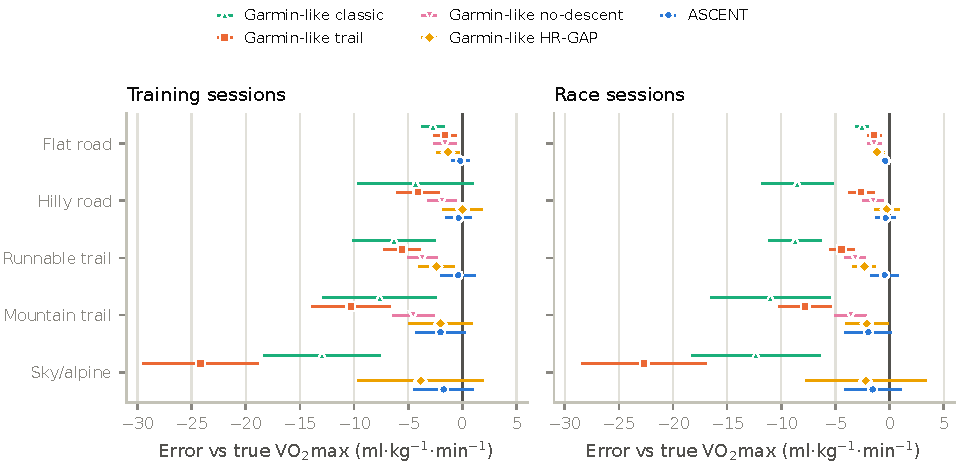
\includegraphics[width=\linewidth]{figures/fig_main_bias.pdf}
\caption{Error of the session estimate (mean $\pm$ SD over \nnRunnersMain{} simulated runners) by course type, for training sessions and races. The no-descent variant produced an estimate in fewer than 1\,\% of alpine sessions and is not shown there.}\label{fig:main}
\end{figure}

\begin{table}[!htbp]\centering\scriptsize
\caption{Main comparison: mean error (SD) [RMSE] in \unit, \nnRunnersMain{} runners per cell. Each method is scored on the sessions where it produced an estimate; n/a: fewer than 10 estimates.}\label{tab:main}
\begin{tabular}{llrrrrr}
\toprule
 & & \multicolumn{4}{c}{Garmin-like reconstructions} & \\ \cmidrule(lr){3-6}
Course & Session & Classic & Trail & No-descent & HR-GAP & ASCENT \\
\midrule
Flat road & training & $-$2.7 (1.0) [2.9] & $-$1.6 (1.0) [1.9] & $-$1.6 (1.0) [1.9] & $-$1.3 (1.1) [1.7] & $-$0.2 (0.8) [0.9] \\
 & race & $-$2.5 (0.6) [2.6] & $-$1.4 (0.6) [1.6] & $-$1.4 (0.6) [1.6] & $-$1.2 (0.7) [1.3] & $-$0.4 (0.5) [0.6] \\
\addlinespace[2pt]
Hilly road & training & $-$4.3 (5.4) [6.9] & $-$4.1 (2.0) [4.6] & $-$1.9 (1.3) [2.3] & +0.0 (1.8) [1.8] & $-$0.3 (1.2) [1.2] \\
 & race & $-$8.5 (3.3) [9.2] & $-$2.6 (1.2) [2.9] & $-$1.5 (1.0) [1.8] & $-$0.3 (1.2) [1.2] & $-$0.4 (0.9) [1.0] \\
\addlinespace[2pt]
Runnable trail & training & $-$6.3 (3.8) [7.4] & $-$5.6 (1.7) [5.8] & $-$3.7 (1.4) [3.9] & $-$2.4 (1.7) [2.9] & $-$0.4 (1.6) [1.6] \\
 & race & $-$8.7 (2.5) [9.1] & $-$4.4 (1.1) [4.6] & $-$3.2 (1.0) [3.3] & $-$2.3 (1.1) [2.6] & $-$0.5 (1.3) [1.4] \\
\addlinespace[2pt]
Mountain trail & training & $-$7.7 (5.3) [9.3] & $-$10.3 (3.7) [10.9] & $-$4.5 (1.9) [4.9] & $-$2.0 (3.0) [3.6] & $-$2.0 (2.3) [3.1] \\
 & race & $-$11.0 (5.6) [12.3] & $-$7.8 (2.5) [8.2] & $-$3.6 (1.5) [3.9] & $-$2.1 (2.0) [2.9] & $-$2.0 (2.2) [2.9] \\
\addlinespace[2pt]
Sky/alpine & training & $-$13.0 (5.4) [14.0] & $-$24.2 (5.3) [24.8] & n/a & $-$3.9 (5.8) [7.0] & $-$1.7 (2.8) [3.3] \\
 & race & $-$12.3 (6.0) [13.7] & $-$22.7 (5.8) [23.4] & n/a & $-$2.2 (5.6) [6.0] & $-$1.6 (2.6) [3.0] \\
\bottomrule
\end{tabular}
\end{table}

\subsection{What causes the watch's penalty}\label{sec:attr}
Figure~\ref{fig:attr} decomposes the biases of two reconstructions, the trail and no-descent variants. The contribution of a mechanism is the change in bias when that mechanism is removed from the simulated world, with everything else held fixed by common random numbers. This measure is meaningful only for mechanisms the estimator does not itself correct.

We therefore leave two things out. Altitude is omitted, because both variants correct for it and removing it from the world makes them over-correct. \ascent{} is not shown, because its fixed priors (terrain factor, descent model, altitude) would make such bars mix each mechanism with \ascent's own correction; its ablation and sensitivity analysis (Appendix~\ref{app:supp}) answer the question better.

For the trail variant on mountain trails:
\begin{itemize}[leftmargin=*]
\item the HR excess on descents contributes \nattrGtrailmountainecc{} \unit, cardiac drift \nattrGtrailmountaindrift, terrain roughness \nattrGtrailmountainterrain{} and GPS shortening \nattrGtrailmountaingpsbias;
\item excluding altitude, all contributions add up to \nattrSumGtrailmountain{}, close to the variant's total bias of \nattrAllGtrailmountain{} in this experiment;
\item on alpine courses the descent excess (\nattrGtrailskyrunecc) and drift (\nattrGtrailskyrundrift) dominate.
\end{itemize}
Discarding descents removes most of the descent contribution (\nattrGtrailnodescmountainecc{} on mountain trails), but drift (\nattrGtrailnodescmountaindrift), terrain (\nattrGtrailnodescmountainterrain) and GPS shortening (\nattrGtrailnodescmountaingpsbias) remain. The HR-lag bars are small and slightly positive, probably because the steadiness filter discards most transient windows.

\begin{figure}[!htbp]\centering
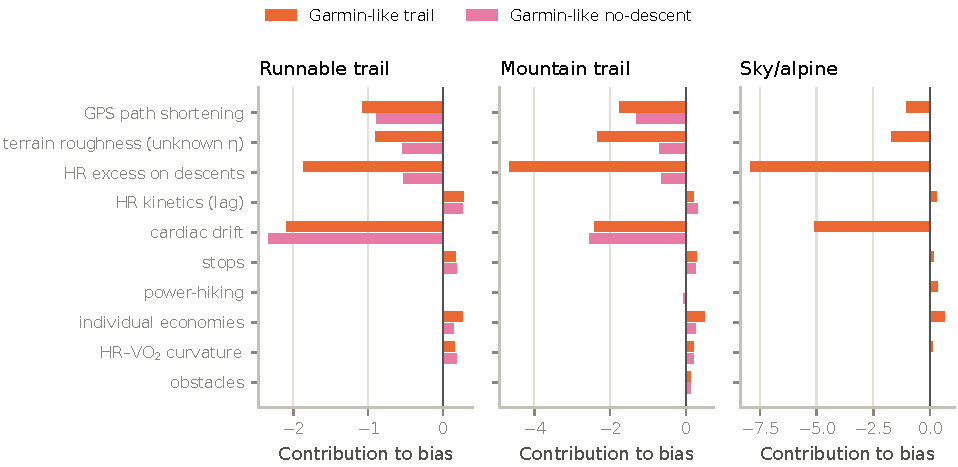
\includegraphics[width=\linewidth]{figures/fig_attribution.pdf}
\caption{Contribution of each mechanism to the bias of two Garmin-like reconstructions (bias with all mechanisms minus bias with the mechanism switched off), training sessions, 60 runners per course type, common random numbers. Altitude is omitted because both variants correct for it. The no-descent variant gives no estimate on alpine courses.}\label{fig:attr}
\end{figure}

\subsection{The displayed value over a training block}
Figure~\ref{fig:long} reproduces the user experience. With a constant-gain smoother, the Garmin-like trail display rises after road sessions (mean \nlongChgRoadGarmin{} points) and falls after almost every mountain-trail session: mean change \nlongChgMtnGarmin{} points, and \nlongDropMtnGarmin\,\% of mountain sessions lowered the rounded value by at least one point. It also drops after races (mean change \nlongChgRaceGarmin{} with race-day HR inflation). Over the block its error is \nlongBiasGarmin{} \unit{} on average (RMSE \nlongRmseGarmin). The no-descent display behaves better but still drops after mountain sessions (mean change \nlongChgMtnGarminND{}; \nlongDropMtnGarminND\,\% of them; RMSE \nlongRmseGarminND).

With \ascent{} and the Kalman tracker, the mean change after a mountain session is \nlongChgMtnKalman{} and the RMSE \nlongRmseKalman; \nlongDropMtnKalman\,\% of mountain sessions lowered the rounded display, against \nlongDropMtnGarmin\,\% for the Garmin-like trail display. When race-day HR is inflated, races still pull the plain tracker down (mean change \nlongChgRaceKalman; \nlongDropRaceKalman\,\% of races lowered the display). The race-aware tracker removes this: mean change \nlongChgRaceRace{}, \nlongDropRaceRace\,\% of races and \nlongDropMtnRace\,\% of mountain sessions lowered the display, against \nlongDropRaceGarmin\,\% and \nlongDropMtnGarmin\,\% for the Garmin-like trail display.

\begin{figure}[!htbp]\centering
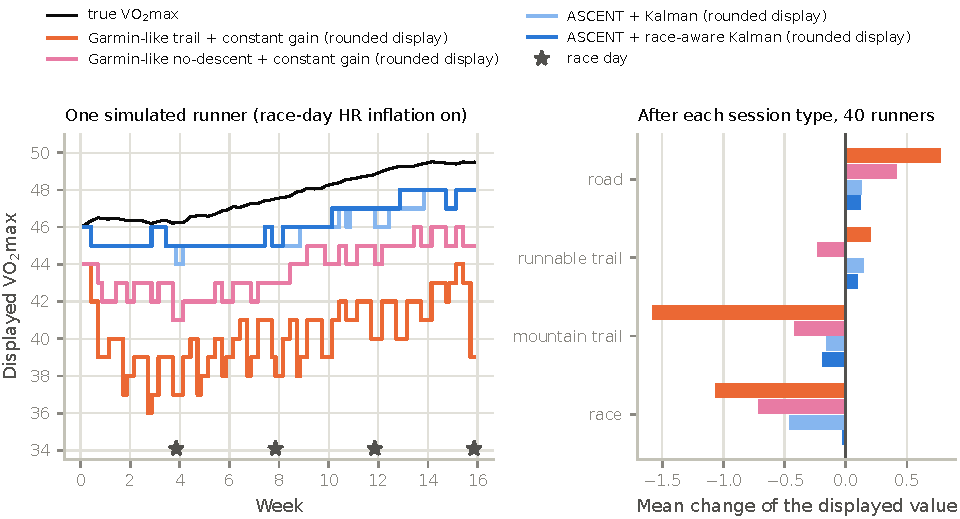
\includegraphics[width=\linewidth]{figures/fig_longitudinal.pdf}
\caption{Displayed \VOmax{} over a 16-week block. Left: one simulated runner (rounded displays, race-day HR inflation on). Right: mean change of the rounded display after each session type, 40 runners.}\label{fig:long}
\end{figure}

\subsection{Structural mismatch}\label{sec:mismatch}
Table~\ref{tab:mismatch} repeats the comparison in worlds whose functional forms differ from \ascent's. Each method is scored on the sessions where it produced an estimate, and the Valid column gives that share. \ascent{} produced an estimate in every session. The Garmin-like methods lost many sessions only when walking and running cadences overlapped: slow running classified as walking broke up their steady windows, and only \nmmCovCadOverlapmountain\,\% of mountain and \nmmCovCadOverlapskyrun\,\% of alpine sessions kept an estimate. The comparisons below are therefore paired: they use the sessions where both the HR-calibrated GAP variant and \ascent{} produced an estimate.

Two changes hurt \ascent{} more than the Garmin-like reconstructions, because \ascent{} leans on climbs and on hiking windows.
\begin{itemize}[leftmargin=*]
\item \emph{Uphill cost 10\,\% above Minetti's at steep grades.} \ascent's mountain-trail bias grew from \nmmBasemountainASCENT{} to \nmmCTiltUpmountainASCENT{} \unit{} (RMSE \nmmCRTiltUpmountainASCENT), against \nmmCTiltUpmountainGtrailhrgap{} (RMSE \nmmCRTiltUpmountainGtrailhrgap) for the HR-calibrated GAP variant.
\item \emph{Overlapping walking and running cadences.} Slow uphill running is then partly classified as walking and costed too low: \ascent's mountain bias was \nmmCCadOverlapmountainASCENT{} (RMSE \nmmCRCadOverlapmountainASCENT), against \nmmCCadOverlapmountainGtrailhrgap{} (RMSE \nmmCRCadOverlapmountainGtrailhrgap). In the sessions the Garmin-like methods dropped, \ascent{} still returned an estimate, but a worse one: on flat roads its RMSE was \nmmRDropCadOverlaproadflat{} there, against \nmmCRCadOverlaproadflatASCENT{} in the other sessions.
\end{itemize}
With all changes combined, the HR-calibrated GAP variant was the more accurate method on mountain trails (RMSE \nmmCRAllMismountainGtrailhrgap{} vs.\ \nmmCRAllMismountainASCENT), and the two were level on runnable trails (\nmmCRAllMistrailrunnableGtrailhrgap{} vs.\ \nmmCRAllMistrailrunnableASCENT). \ascent{} remained the more accurate method on alpine courses (\nmmCRAllMisskyrunASCENT{} vs.\ \nmmCRAllMisskyrunGtrailhrgap), where the Garmin-like methods produced an estimate in only \nmmCovAllMisskyrun\,\% of sessions.

The other changes (an uphill cost 10\,\% below Minetti's, a linear descent excess, a steeper altitude loss and accelerating drift) left the ranking unchanged, although the cheaper uphill cost made \ascent{} overestimate on alpine courses (\nmmTiltDownskyrunASCENT). \ascent's advantage on mountain and runnable trails is therefore conditional on its uphill cost model and on clean gait detection. Both can be checked on a watch: the first with an internal consistency test (the estimate from climbing windows against the estimate from level windows of the same session), the second from the cadence distribution.

\begin{table}[!htbp]\centering\scriptsize
\caption{Structural mismatch: mean error [RMSE] (\unit) in worlds whose functional forms differ from \ascent's, \nnMismatch{} runners, training and races pooled. Each method is scored on the sessions where it produced an estimate. Valid: percentage of sessions with an estimate for the classic, trail and HR-GAP variants (one shared window selection) / for the no-descent variant; \ascent{} produced an estimate in every session. n/a: fewer than 10 estimates. The \ascent{} values quoted in the text for the overlapping-cadence and combined worlds are on the sessions where the HR-GAP variant also produced an estimate, and differ slightly from this table.}\label{tab:mismatch}
\begin{tabular}{@{}lrrrrrr@{}}
\toprule
World / course & Valid (\%) & Classic & Trail & No-descent & HR-GAP & ASCENT \\
\midrule
\multicolumn{7}{@{}l}{\textit{baseline}} \\
\quad Flat road & 100/100 & $-$2.8 [2.9] & $-$1.7 [1.9] & $-$1.7 [1.9] & $-$1.4 [1.7] & $-$0.4 [0.8] \\
\quad Runnable trail & 100/100 & $-$8.1 [8.8] & $-$5.2 [5.4] & $-$3.6 [3.8] & $-$2.6 [2.9] & $-$0.4 [1.6] \\
\quad Mountain trail & 100/85 & $-$10.3 [11.8] & $-$9.2 [9.8] & $-$4.0 [4.4] & $-$2.4 [3.4] & $-$1.9 [3.0] \\
\quad Sky/alpine & 97/4 & $-$13.6 [14.8] & $-$24.5 [25.1] & n/a & $-$4.1 [7.2] & $-$1.5 [3.1] \\
\addlinespace[3pt]
\multicolumn{7}{@{}l}{\textit{uphill cost $+10$\,\%}} \\
\quad Flat road & 100/100 & $-$2.8 [2.9] & $-$1.7 [1.9] & $-$1.7 [1.9] & $-$1.4 [1.7] & $-$0.4 [0.8] \\
\quad Runnable trail & 100/100 & $-$8.1 [9.0] & $-$5.4 [5.6] & $-$4.3 [4.5] & $-$2.8 [3.2] & $-$1.5 [2.3] \\
\quad Mountain trail & 100/82 & $-$9.5 [11.3] & $-$9.1 [9.7] & $-$5.2 [5.5] & $-$2.4 [3.6] & $-$4.1 [4.7] \\
\quad Sky/alpine & 95/2 & $-$12.2 [13.7] & $-$23.6 [24.3] & n/a & $-$2.5 [6.5] & $-$5.3 [6.0] \\
\addlinespace[3pt]
\multicolumn{7}{@{}l}{\textit{uphill cost $-10$\,\%}} \\
\quad Flat road & 100/100 & $-$2.8 [2.9] & $-$1.7 [1.9] & $-$1.7 [1.9] & $-$1.4 [1.7] & $-$0.3 [0.8] \\
\quad Runnable trail & 100/100 & $-$8.3 [8.8] & $-$4.8 [5.1] & $-$2.7 [3.1] & $-$2.3 [2.7] & +0.5 [1.8] \\
\quad Mountain trail & 100/87 & $-$11.0 [12.3] & $-$8.9 [9.7] & $-$2.6 [3.3] & $-$2.3 [3.4] & +0.6 [3.2] \\
\quad Sky/alpine & 97/4 & $-$15.2 [16.1] & $-$25.0 [25.6] & n/a & $-$5.5 [7.8] & +2.6 [4.3] \\
\addlinespace[3pt]
\multicolumn{7}{@{}l}{\textit{descent HR excess linear in grade}} \\
\quad Flat road & 100/100 & $-$2.8 [2.9] & $-$1.7 [1.9] & $-$1.7 [1.9] & $-$1.4 [1.7] & $-$0.4 [0.8] \\
\quad Runnable trail & 100/100 & $-$8.1 [8.8] & $-$5.2 [5.4] & $-$3.6 [3.8] & $-$2.6 [3.0] & $-$0.5 [1.6] \\
\quad Mountain trail & 100/85 & $-$10.4 [11.9] & $-$9.4 [10.0] & $-$4.0 [4.4] & $-$2.5 [3.5] & $-$1.9 [3.0] \\
\quad Sky/alpine & 98/4 & $-$14.3 [15.4] & $-$25.0 [25.6] & n/a & $-$4.8 [7.6] & $-$1.5 [3.1] \\
\addlinespace[3pt]
\multicolumn{7}{@{}l}{\textit{steeper altitude loss (quadratic)}} \\
\quad Flat road & 100/100 & $-$2.9 [3.0] & $-$1.8 [2.0] & $-$1.8 [2.0] & $-$1.5 [1.7] & $-$0.4 [0.7] \\
\quad Runnable trail & 100/100 & $-$8.2 [8.9] & $-$5.3 [5.5] & $-$3.7 [4.0] & $-$2.7 [3.1] & $-$0.4 [1.5] \\
\quad Mountain trail & 100/82 & $-$10.4 [12.2] & $-$9.8 [10.3] & $-$4.8 [5.1] & $-$3.0 [4.0] & $-$2.6 [3.5] \\
\quad Sky/alpine & 98/2 & $-$15.9 [16.8] & $-$26.5 [27.1] & n/a & $-$7.0 [8.9] & $-$2.4 [3.8] \\
\addlinespace[3pt]
\multicolumn{7}{@{}l}{\textit{accelerating drift (quadratic)}} \\
\quad Flat road & 100/100 & $-$2.4 [2.5] & $-$1.2 [1.5] & $-$1.2 [1.5] & $-$0.9 [1.3] & +0.3 [0.8] \\
\quad Runnable trail & 100/100 & $-$8.1 [8.7] & $-$5.2 [5.5] & $-$3.6 [3.8] & $-$2.5 [2.9] & +0.8 [1.9] \\
\quad Mountain trail & 100/85 & $-$10.5 [11.9] & $-$9.5 [10.1] & $-$4.1 [4.6] & $-$2.6 [3.7] & $-$0.4 [2.5] \\
\quad Sky/alpine & 98/4 & $-$18.7 [19.8] & $-$28.1 [28.8] & n/a & $-$9.9 [11.9] & +1.4 [3.6] \\
\addlinespace[3pt]
\multicolumn{7}{@{}l}{\textit{overlapping walk/run cadence}} \\
\quad Flat road & 78/78 & $-$2.7 [2.8] & $-$1.5 [1.8] & $-$1.5 [1.8] & $-$1.2 [1.5] & $-$1.0 [1.6] \\
\quad Runnable trail & 92/58 & $-$2.1 [4.8] & $-$7.5 [7.9] & $-$4.2 [4.4] & $-$1.6 [2.9] & $-$2.1 [3.0] \\
\quad Mountain trail & 76/11 & $-$3.2 [5.8] & $-$12.8 [13.5] & $-$4.7 [5.1] & $-$0.8 [4.0] & $-$4.4 [5.2] \\
\quad Sky/alpine & 55/0 & $-$9.5 [11.2] & $-$23.9 [24.5] & n/a & $-$1.1 [6.3] & $-$2.7 [4.8] \\
\addlinespace[3pt]
\multicolumn{7}{@{}l}{\textit{all of the above ($+10$\,\%)}} \\
\quad Flat road & 78/78 & $-$2.2 [2.4] & $-$1.1 [1.4] & $-$1.1 [1.4] & $-$0.8 [1.1] & $-$0.5 [1.3] \\
\quad Runnable trail & 90/58 & $-$1.2 [4.7] & $-$6.8 [7.3] & $-$4.5 [4.6] & $-$0.9 [2.9] & $-$2.0 [3.2] \\
\quad Mountain trail & 78/12 & $-$2.5 [6.0] & $-$12.3 [12.9] & $-$5.6 [6.0] & $-$0.1 [4.3] & $-$5.7 [6.4] \\
\quad Sky/alpine & 34/0 & $-$14.7 [15.9] & $-$28.0 [28.6] & n/a & $-$7.0 [9.5] & $-$4.6 [5.9] \\
\bottomrule
\end{tabular}
\end{table}

% =========================================================================================
\section{Terrain invariance on \nnFitrecRuns{} runs of \nnFitrecRunners{} Endomondo users}\label{sec:fitrec}

The simulation can only test the method against its own assumptions. To test it on real runners we used the FitRec dataset \citep{ni2019}: 253\,020 workouts of 1\,104 Endomondo users (2006--2016) with heart rate and GPS, released for academic use. It has no laboratory reference, so it cannot say which method is right. It can say whether a method gives the same runner the same number on flat and on hilly runs in the same weeks, which is the property the watch lacks.

\subsection{Data and protocol}
We kept the running workouts with HR, GPS and altitude (104\,498 runs of 848 users), rebuilt distance from the GPS track (position jumps capped at 7\,m\,s$^{-1}$) and used the recorded altitude, whose source (barometric or GPS) depends on the device and is unknown. The data have no cadence, no resting or maximal HR, no terrain label and no race flag. The protocol was fixed before any estimate was computed, with two exceptions stated below (the altitude-plausibility filters and the no-gait-label run of \ascent, both added after a first pass):
\begin{itemize}[leftmargin=*]
\item runs of at least 25 min, at least 80\,\% of the time moving, median HR above 100 bpm, and plausible altitude data: mean altitude between $-100$ and 3500 m, climbing at most 150 m\,km$^{-1}$, total ascent and descent within 50\,\% of each other, and altitude roughness below 5 m. Some devices record altitude garbage (mean ``altitudes'' of 7000 m), which inflated the steep bin for every method in a first pass. The workouts were resampled to 500 points by the dataset's authors, so the spacing grows with duration; runs with a mean spacing above 30 s (longer than about 4 h) were excluded and the gap flag of the preprocessing was relaxed to 35 s;
\item terrain from the climbing per km of the smoothed altitude: \emph{flat} up to 8 m\,km$^{-1}$, \emph{hilly} from 25 m\,km$^{-1}$, \emph{steep} from 40 m\,km$^{-1}$; runs in between are \emph{intermediate};
\item runners with at least five flat and five hilly runs; per runner, the most recent 30 flat, 60 hilly and 20 intermediate runs, so that terrains interleave in time. This gives \nnFitrecRuns{} runs of \nnFitrecRunners{} runners (median \nfitrecRunsPerRunner{} runs each, median duration \nfitrecDurMed{} min): \nnFitrecFlat{} flat, \nnFitrecMid{} intermediate and \nnFitrecHilly{} hilly, of which \nnFitrecSteep{} steep;
\item \HRmax{} per runner is the 95th percentile of the per-run 99th-percentile HR over all the runner's runs (median \nfitrecHrmaxMed{} bpm); \HRrest{} is 55 bpm for everybody. Both anchors are constant within a runner, so they shift levels, not terrain differences;
\item surface class ``road'' and accelerometer factor 1 for every run, since the terrain is unknown. The test therefore covers the grade, gait, descent, kinetics and drift mechanisms, not the terrain factor;
\item the Garmin-like reconstructions need a walking filter. Without cadence we labelled slow, steep uphill (below 1.9 m\,s$^{-1}$ on grades above 8\,\%) as walking, as a watch with cadence would exclude it. \ascent{} was run twice: with the same labels (its frozen configuration, \ascent$^{\dagger}$) and with no gait labels at all (\ascent). The second run, like the altitude filters above, was added after the diagnosis of a first pass (Section~\ref{sec:fitrecgait}), so the test is not pre-registered in the strict sense; the frozen column is reported alongside.
\end{itemize}
Three statistics, all within runner: (a) \emph{dose--response}: every run above 8 m\,km$^{-1}$ minus the mean of the same runner's flat runs within $\pm30$ days (``the same month'' below), averaged per runner, then the 10\,\% trimmed mean and the median across runners in four climbing bins (confidence intervals are those of the untrimmed mean); (b) \emph{slope}: for every runner with at least 12 valid runs (157 of 158), a regression of the estimate on climbing per km with a linear time trend and duration as covariates, the slope per 10 m\,km$^{-1}$ averaged across runners with a 95\,\% CI; (c) a \emph{noise floor}: the same gap between two random halves of each runner's flat runs.

\subsection{Results}
Table~\ref{tab:fitrec} and Figure~\ref{fig:fitrec} summarise the test. The flat-versus-flat control sets the noise floor of a per-runner gap: an SD of about \nfrNoiseSdGflat{} \unit{} for the reconstructions and \nfrNoiseSdASCENT{} for \ascent{} (Table~\ref{tab:fitrec}, last row).
\begin{itemize}[leftmargin=*]
\item \emph{Classic variant.} A clean dose--response: \nfrTrimAGflat, \nfrTrimBGflat, \nfrTrimCGflat{} and \nfrTrimDGflat{} \unit{} in the four climbing bins, and a slope of \nfrSlopeGflat{} [\nfrSlopeLoGflat, \nfrSlopeHiGflat] per 10 m\,km$^{-1}$. This is the classic method's penalty, measured in \nnFitrecRunners{} people.
\item \emph{Trail variant} (metabolic grade adjustment on the path speed): \nfrTrimCGtrail{} on runs climbing 25--40 m\,km$^{-1}$ and \nfrTrimDGtrail{} on steep runs. On real steep runs the metabolic adjustment removes almost nothing, as the simulation predicted (Section~\ref{sec:attr}).
\item \emph{No-descent variant}: invariant, \nfrTrimCGnodesc{} and \nfrTrimDGnodesc, but by cancellation. With duration held fixed it rises with climbing (\nfrSlopeGnodesc{} [\nfrSlopeLoGnodesc, \nfrSlopeHiGnodesc] per 10 m\,km$^{-1}$) and falls with duration (\nfrPerHourGnodesc{} per hour), and steep runs are longer. It also produced an estimate in only \nfrCovHillyGnodesc\,\% of hilly runs.
\item \emph{HR-calibrated GAP}: \nfrTrimCGhrgap{} on runs climbing 25--40 m\,km$^{-1}$ and \nfrTrimDGhrgap{} on steep runs; slope \nfrSlopeGhrgap{} [\nfrSlopeLoGhrgap, \nfrSlopeHiGhrgap].
\item \emph{\ascent{}} (no gait labels): \nfrTrimAASCENT, \nfrTrimBASCENT, \nfrTrimCASCENT{} and \nfrTrimDASCENT{} [95\,\% CI of the mean \nfrLoDASCENT, \nfrHiDASCENT]; slope \nfrSlopeASCENT{} [\nfrSlopeLoASCENT, \nfrSlopeHiASCENT]. It is within 0.5 \unit{} of the flat runs up to 25 m\,km$^{-1}$, loses about half as much as the trail variant on steep runs, and is close to the HR-calibrated GAP. It produced an estimate in \nfrCovHillyASCENT\,\% of runs above 25 m\,km$^{-1}$ against \nfrCovHillyGhrgap\,\% for the classic, trail and HR-GAP reconstructions (\nfrCovHillyGnodesc\,\% for the no-descent variant), and its duration effect was the smallest (\nfrPerHourASCENT{} per hour [\nfrPerHourLoASCENT, \nfrPerHourHiASCENT], against \nfrPerHourGflat{} to \nfrPerHourGnodesc{} for the reconstructions). Its session-to-session spread within a runner on flat runs was larger (SD \nfrSessSdASCENT{} vs.\ \nfrSessSdGhrgap{} \unit).
\item \emph{\ascent$^{\dagger}$} (frozen configuration, with the speed-based walking labels): \nfrTrimCASCENTgh{} and \nfrTrimDASCENTgh, close to the trail variant on steep runs.
\end{itemize}
The ordering of the simulation holds in part. The classic and trail reconstructions lose most on hilly ground; among the methods that keep descents, \ascent{} and the HR-calibrated GAP lose least; the no-descent variant is level, by the cancellation described above. But no method is invariant above 40 m\,km$^{-1}$ in these data, where \ascent{} still loses about 3 \unit{} relative to the same runner's flat runs, and the simplest reconstruction, dropping descents, is level with the flat runs there.

\begin{table}[!htbp]\centering\scriptsize\setlength{\tabcolsep}{3.5pt}
\caption{Terrain invariance on FitRec: estimate minus the runner's flat runs of the same month, by climbing bin (10\,\% trimmed mean (median) over runners, \unit); within-runner slope on climbing with duration held fixed; duration effect; share of runs above 25 m\,km$^{-1}$ with an estimate; session-to-session SD within runner on flat runs; SD of the flat-versus-flat control gap. $\dagger$: \ascent{} with the speed-based walking labels of its frozen configuration.}\label{tab:fitrec}
\begin{tabular}{@{}lrrrrrr@{}}
\toprule
Climbing (m\,km$^{-1}$) & Classic & Trail & No-descent & HR-GAP & ASCENT & ASCENT$^{\dagger}$ \\
\midrule
8--15 & $-$0.4 ($-$0.2) & +0.0 (+0.0) & +0.5 (+0.4) & +0.4 (+0.4) & +0.4 (+0.4) & +0.4 (+0.4) \\
15--25 & $-$1.9 ($-$1.8) & $-$0.9 ($-$0.6) & +0.8 (+0.8) & +0.3 (+0.5) & $-$0.4 ($-$0.1) & $-$0.6 ($-$0.3) \\
25--40 & $-$4.3 ($-$4.2) & $-$3.0 ($-$2.3) & +0.4 (+0.3) & $-$0.9 ($-$0.6) & $-$1.4 ($-$1.1) & $-$2.0 ($-$2.2) \\
$>$40 & $-$7.4 ($-$6.4) & $-$6.8 ($-$7.8) & $-$0.1 (+0.0) & $-$2.6 ($-$3.6) & $-$3.3 ($-$3.5) & $-$5.9 ($-$6.4) \\
\midrule
Slope per 10 m\,km$^{-1}$ & $-$1.4 & $-$0.9 & +0.7 & $-$0.1 & +0.0 & $-$0.3 \\
\quad 95\,\% CI & [$-$1.6, $-$1.2] & [$-$1.1, $-$0.6] & [+0.4, +0.9] & [$-$0.3, +0.2] & [$-$0.3, +0.3] & [$-$0.6, +0.1] \\
Duration effect per hour & $-$1.5 & $-$1.7 & $-$1.7 & $-$1.6 & $-$0.6 & $-$0.7 \\
Valid runs, $\geq 25$ m\,km$^{-1}$ (\%) & 87 & 87 & 82 & 87 & 96 & 96 \\
Session SD within runner, flat runs & 3.0 & 3.0 & 3.1 & 3.1 & 3.6 & 3.6 \\
Flat-vs-flat control SD & 2.0 & 2.1 & 2.1 & 2.1 & 2.5 & 2.5 \\
\bottomrule
\end{tabular}
\end{table}

\begin{figure}[!htbp]\centering
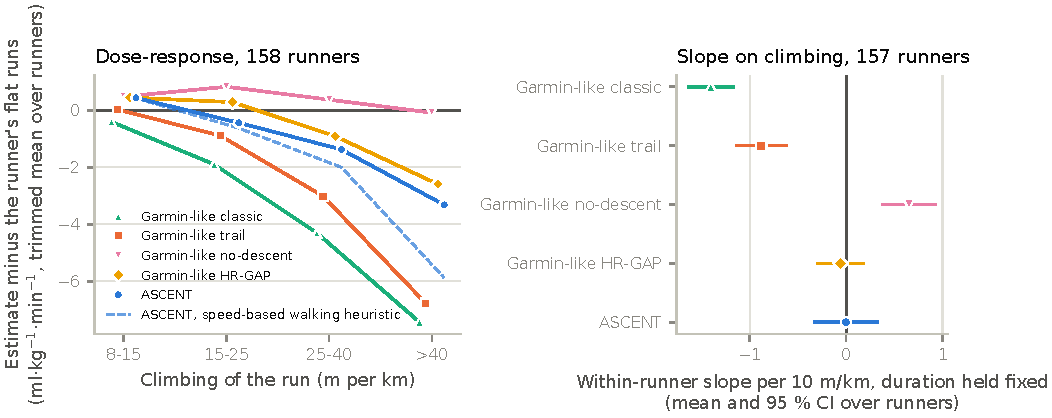
\includegraphics[width=\linewidth]{figures/fig_fitrec.pdf}
\caption{FitRec terrain-invariance test. Left: estimate minus the runner's flat runs of the same month, by climbing of the run (trimmed mean over runners). Right: within-runner slope on climbing per km with duration held fixed, mean and 95\,\% CI over runners.}\label{fig:fitrec}
\end{figure}

\subsection{What \ascent{} gets wrong on steep runs}\label{sec:fitrecgait}
We re-ran the steep runs ($\geq40$ m\,km$^{-1}$) and their paired flat runs with one change to \ascent{} at a time (Table~\ref{tab:fitrecdiag}); every variant is compared with the same variant on the flat runs, so a change that shifts all estimates does not pass for a terrain effect. Three findings:
\begin{itemize}[leftmargin=*]
\item \emph{Gait labels without cadence.} The speed-based heuristic of the frozen configuration labelled slow uphill running as walking, which is costed about 30\,\% lower per metre, and the estimate followed: \nfrDiagMedGaitH{} with the labels against \nfrDiagMedBase{} without. This is the gait-misclassification failure mode of Section~\ref{sec:mismatch}, seen in real data, and the reason \ascent{} now uses no gait labels when cadence is absent. The change was made after this diagnosis.
\item \emph{The HR-lag term.} Without it the gap shrinks to \nfrDiagMedNoLag{} (median; trimmed mean \nfrDiagTrimNoLag). The fitted lag sat at its 120-s cap in \nfrTauCapSteep\,\% of steep runs against \nfrTauCapFlat\,\% of flat runs: on coarsely sampled steep runs the lag is poorly identified and absorbs part of the terrain signal. The profile over $\tau$ needs a tighter prior, or a fixed lag, when the sampling is coarse. We did not change it within this test; Section~\ref{sec:v2} does so on a held-out split.
\item \emph{Surface.} A trail surface class on the steep run alone ($h=1.07$) also removes most of the gap (\nfrDiagMedTrailH). Steep runs are mostly on trails, so part of the residual is the terrain factor the test could not include.
\end{itemize}
Removing the drift term (\nfrDiagMedNoDrift) or excluding descents (\nfrDiagMedNoDesc) changed little. Within a steep run, \ascent's climb-only and flat-only estimates both sat below the runner's flat runs (\nfrDiagMedClimbs{} and \nfrDiagMedFlats), with a median within-run difference of \nfrDiagMedWithin{} between the two (\nfrDiagNWithin{} runners with both estimates): the shortfall is session-wide, not an uphill-cost error alone.

\begin{table}[!htbp]\centering\small
\caption{Steep FitRec runs ($\geq40$ m\,km$^{-1}$, \nfrDiagNBase{} runners): median (10\,\% trimmed mean) over runners of the gap between the steep run and the runner's flat runs of the same month, \ascent{} with one change at a time, the same change applied to the flat runs (\unit). The first two rows are the $>$40 bin of Table~\ref{tab:fitrec}, median first here.}\label{tab:fitrecdiag}
\begin{tabular}{@{}lr@{}}
\toprule
\ascent{} variant & Gap, median (trimmed mean) \\
\midrule
No gait labels (default without cadence) & \nfrDiagMedBase{} (\nfrDiagTrimBase) \\
Speed-based walking labels (frozen configuration) & \nfrDiagMedGaitH{} (\nfrDiagTrimGaitH) \\
No HR lag & \nfrDiagMedNoLag{} (\nfrDiagTrimNoLag) \\
Trail surface class on the steep run ($h=1.07$) & \nfrDiagMedTrailH{} (\nfrDiagTrimTrailH) \\
No drift term & \nfrDiagMedNoDrift{} (\nfrDiagTrimNoDrift) \\
Descents excluded & \nfrDiagMedNoDesc{} (\nfrDiagTrimNoDesc) \\
Climbs only (grade $\geq 4$\,\%) & \nfrDiagMedClimbs{} (\nfrDiagTrimClimbs) \\
Flats only ($-3$ to $4$\,\%) & \nfrDiagMedFlats{} (\nfrDiagTrimFlats) \\
Climbs only minus flats only, within the same run (\nfrDiagNWithin{} runners) & \nfrDiagMedWithin{} (\nfrDiagTrimWithin) \\
\bottomrule
\end{tabular}
\end{table}

% =========================================================================================
\section{\texorpdfstring{\ascent{}}{ASCENT} v2: what the experiments changed}\label{sec:v2}

The Endomondo test exposed three settings of the frozen configuration (speed-based gait labels without cadence, a free HR lag on coarsely sampled runs, and an unknown surface); the simulation showed that the lag could be fixed at no cost. This section turns them into a revised configuration, developed on one half of the Endomondo runners and confirmed on the other half and on the simulation. The revision keeps the model of Section~\ref{sec:ascent}; relative to the frozen configuration it changes three settings and one default. Throughout, \emph{v1} is the configuration of Section~\ref{sec:ascent} run with no gait labels (the \ascent{} column of Table~\ref{tab:fitrec}); \ascent$^{\dagger}$ is the same configuration with the speed-based labels; \emph{v2} is this section's configuration.

\subsection{Changes}
\begin{enumerate}[leftmargin=*]
\item \emph{No gait labels without cadence} (Section~\ref{sec:fitrecgait}). With cadence, gait comes from cadence as before.
\item \emph{HR lag fixed at the literature mean, 55 s} \citep{hunt2015}, instead of a profile over seven values with a prior. The free lag sat at its cap in \nfrTauCapSteep\,\% of steep Endomondo runs and absorbed terrain signal; in the simulation, fixing it cost nothing (Table~\ref{tab:v2sim}).
\item \emph{Surface class ``auto'' when the terrain is unknown.} The prior on the horizontal-cost factor $h$ is interpolated between the road value (1.00) and the trail value (1.07) by the climbing of the session, from 8 to 40 m\,km$^{-1}$, the flat and steep thresholds of Section~\ref{sec:fitrec}. When the sport type is known (a watch's ``Trail Run'' profile, a Strava sport type), the labelled class is used as before: the climbing of a session is a crude proxy for its surface, and Section~\ref{sec:v2res} shows where it fails.
\item \emph{Tighter prior on cardiac drift}, sd 0.03 instead of 0.05 per hour, with the same mean.
\end{enumerate}

\subsection{Development protocol}
The Endomondo runners of Section~\ref{sec:fitrec} were split by the parity of their user id: \nnVdevRunners{} runners form the development half and \nnVtestRunners{} the test half. Candidates were compared on the development half only, on flat and hilly runs, by the within-runner gap of Section~\ref{sec:fitrec} in the 25--40 and $>$40 m\,km$^{-1}$ bins (\nnVdevHilly{} and \nnVdevSteep{} runners with pairs), the session-to-session SD within runner on flat runs, and the share of hilly runs with an estimate (Table~\ref{tab:v2dev}). The descent cost $\lambda$ (0.5, 0.75, 1) and the Huber constant ($c=2$, 1.2) were also varied and left unchanged: they moved the gaps by at most 0.4 \unit. Two further rows are diagnostics, not candidates: without the drift term the session SD falls to \nvdevSdTAnd{} but the level drops by two units; without the error-budget weights the steep gap doubles. The configuration was chosen by the smallest gap in the $>$40 bin among those with the lowest session SD; the surface prior alone leaves \nvdevDA{} on steep runs. The chosen configuration (v2) was then frozen and run once on the test half and on the simulation sessions of Section~\ref{sec:simres} (same seeds).

\begin{table}[!htbp]\centering\footnotesize
\caption{Development half of the Endomondo runners (\nnVdevRunners{} runners): gap to the runner's flat runs in the 25--40 and $>$40 m\,km$^{-1}$ bins (10\,\% trimmed mean, \unit), session-to-session SD within runner on flat runs, share of runs above 25 m\,km$^{-1}$ with an estimate, and mean level on flat runs. No gait labels in every row.}\label{tab:v2dev}
\begin{tabular}{@{}lrrrrr@{}}
\toprule
Candidate & 25--40 & $>$40 & Session SD & Valid hilly (\%) & Level \\
\midrule
v1 & $-$1.9 & $-$3.9 & 3.68 & 96 & 59.9 \\
lag fixed at 55 s & $-$1.3 & $-$3.3 & 3.68 & 95 & 60.1 \\
lag prior tightened (sd 15 s, cap 80 s) & $-$1.6 & $-$3.7 & 3.67 & 95 & 60.1 \\
surface `auto' & +0.3 & $-$1.5 & 3.68 & 95 & 59.9 \\
lag fixed + `auto' & +0.8 & $-$1.3 & 3.68 & 94 & 60.1 \\
lag fixed + `auto' + $\lambda=0.75$ & +1.0 & $-$1.3 & 3.69 & 94 & 60.2 \\
lag fixed + `auto' + $\lambda=1$ & +1.2 & $-$1.3 & 3.69 & 94 & 60.4 \\
lag fixed + `auto' + Huber $c=1.2$ & +0.6 & $-$1.4 & 3.68 & 95 & 60.1 \\
lag fixed + `auto' + drift sd 0.03/h (= v2; $\lambda=0.5$) & +0.9 & $-$1.1 & 3.57 & 95 & 59.8 \\
lag fixed + `auto', no drift (diagnostic) & +1.1 & $-$1.2 & 3.40 & 96 & 58.1 \\
lag fixed + `auto', no weights (diagnostic) & +0.1 & $-$2.7 & 3.70 & 94 & 60.0 \\
\bottomrule
\end{tabular}
\end{table}

\subsection{Results}\label{sec:v2res}
\paragraph{Test half.} Table~\ref{tab:v2test}. v1 reproduces the dose--response of Section~\ref{sec:fitrec} on these runners (\nvtestCOne{} and \nvtestDOne{} in the two upper bins); v2 is within about $\pm1.5$ \unit{} of the runner's flat runs in every bin (trimmed means \nvtestATwo, \nvtestBTwo, \nvtestCTwo{} and \nvtestDTwo). The residual is an over-correction on runs climbing 25--40 m\,km$^{-1}$ (\nvtestCTwo{} [\nvtestLoCTwo, \nvtestHiCTwo]): the climbing proxy assigns a partly-trail prior to hilly runs that may be on roads. The session SD fell a little (\nvtestSdTwo{} vs.\ \nvtestSdOne) and coverage is essentially unchanged (\nvtestCovTwo{} vs.\ \nvtestCovOne\,\%). The same table gives the HR-calibrated GAP and no-descent reconstructions on the same runners. Paired per runner on the same runs, v2 minus HR-GAP is \nvpairD{} [\nvpairLoD, \nvpairHiD] \unit{} in the $>$40 bin (\nvpairND{} runners), \nvpairC{} [\nvpairLoC, \nvpairHiC] in the 25--40 bin, \nvpairB{} [\nvpairLoB, \nvpairHiB] in the 15--25 bin and \nvpairA{} [\nvpairLoA, \nvpairHiA] in the 8--15 bin; in the 25--40 bin the difference is v2 over-correcting against HR-GAP under-correcting by about the same amount, and in the 15--25 bin it is mostly v2's over-correction. Over the no-descent reconstruction the advantage is coverage (\nvtestCovTwo{} vs.\ \nvtestCovGnodesc\,\% of runs above 25 m\,km$^{-1}$), not invariance.

\begin{table}[!htbp]\centering\scriptsize\setlength{\tabcolsep}{2.5pt}
\caption{Test half of the Endomondo runners (\nnVtestRunners{} runners): gap to the runner's flat runs of the same month by climbing bin (10\,\% trimmed mean [95\,\% CI of the mean] over runners, \unit), session SD within runner on flat runs and share of hilly runs with an estimate. v1 and v2 as defined above; the two reconstructions on the same runs. Valid: share of runs above 25 m\,km$^{-1}$ with an estimate.}\label{tab:v2test}
\begin{tabular}{@{}lrrrrrr@{}}
\toprule
Estimator & 8--15 & 15--25 & 25--40 & $>$40 & Sess.\ SD & Valid (\%) \\
\midrule
\ascent{} v1 & +0.0 [$-$0.9, +0.7] & $-$0.9 [$-$2.5, $-$0.1] & $-$1.0 [$-$2.5, +0.6] & $-$2.6 [$-$5.1, $-$0.9] & 3.39 & 97 \\
\ascent{} v2 & +0.3 [$-$0.4, +1.0] & +0.6 [$-$0.9, +1.3] & +1.4 [+0.0, +2.9] & +0.3 [$-$2.1, +2.1] & 3.31 & 96 \\
HR-GAP & +0.0 [$-$0.7, +0.7] & $-$0.2 [$-$1.4, +1.4] & $-$1.2 [$-$2.7, +0.1] & $-$2.5 [$-$4.5, $-$0.6] & 3.05 & 89 \\
No-descent & +0.0 [$-$0.7, +0.7] & +0.4 [$-$0.9, +1.9] & +0.2 [$-$1.4, +1.5] & $-$0.1 [$-$2.7, +3.1] & 3.02 & 85 \\
\bottomrule
\end{tabular}
\end{table}

\paragraph{Simulation.} Table~\ref{tab:v2sim} replays the \nnRunnersMain{} runners of the main comparison. With the surface known, v2 is as accurate as v1 on every course type and a little better on mountain trails (RMSE \nvsimRmountainTwo{} vs.\ \nvsimRmountainOne), so the revision cost nothing in simulation. With the surface set to ``auto'', the proxy misfires where climbing and surface disagree: hilly roads (\nvsimroadhillyTwoAuto, because a road with \nvsimHauto{} as mean $h$ prior is costed as part trail) and runnable trails (\nvsimtrailrunnableTwoAuto, costed as near road). In the structural-mismatch worlds the ranking of Section~\ref{sec:mismatch} is unchanged: on mountain trails v2 has RMSE \nvmmRTiltUpmountainTwo{} with the uphill cost 10\,\% above Minetti's (v1 \nvmmRTiltUpmountainOne, HR-GAP \nvmmRTiltUpmountainGhrgap) and \nvmmRAllMismountainTwo{} with all changes combined (v1 \nvmmRAllMismountainOne, HR-GAP \nvmmRAllMismountainGhrgap).

\begin{table}[!htbp]\centering\small
\caption{Simulation replay (\nnRunnersMain{} runners, training and races pooled): mean error [RMSE] in \unit{} of the HR-calibrated GAP reconstruction, \ascent{} v1, \ascent{} v2 with the known surface class and v2 with the surface set to ``auto''.}\label{tab:v2sim}
\begin{tabular}{@{}lrrrr@{}}
\toprule
Course & HR-GAP & \ascent{} v1 & \ascent{} v2 & \ascent{} v2, surface `auto' \\
\midrule
Flat road & $-$1.2 [1.5] & $-$0.3 [0.7] & $-$0.4 [0.8] & $-$0.4 [0.8] \\
Hilly road & $-$0.1 [1.6] & $-$0.4 [1.1] & $-$0.4 [1.0] & +1.3 [1.6] \\
Runnable trail & $-$2.4 [2.8] & $-$0.4 [1.5] & $-$0.4 [1.3] & $-$1.9 [2.3] \\
Mountain trail & $-$2.1 [3.3] & $-$2.0 [3.0] & $-$1.9 [2.7] & $-$1.9 [2.7] \\
Sky/alpine & $-$3.0 [6.5] & $-$1.6 [3.2] & $-$1.8 [3.2] & $-$1.8 [3.2] \\
\bottomrule
\end{tabular}
\end{table}

\paragraph{When the surface is known.} The climbing proxy is only a fallback. On a watch the activity profile (``Run'' or ``Trail Run'') and, better, an accelerometer roughness index are available, and either takes precedence. A hilly road loop (30 m\,km$^{-1}$ of climbing on asphalt is common) would otherwise receive a partly-trail prior and be costed too high, which is the hilly-road error of Table~\ref{tab:v2sim}.

\paragraph{What v2 does and does not fix.} v2 removes the terrain dependence that v1 kept on steep Endomondo runs, at no cost in the simulation, and with slightly less session noise. It does so with a proxy that will misjudge hilly roads and flat trails; a terrain measurement (an accelerometer roughness index, as Garmin's trail estimate uses) belongs in its place. The session noise remains larger than that of the reconstructions, and the uphill cost model and the descent HR excess are unchanged, so the conditional conclusions of Sections~\ref{sec:mismatch} and \ref{sec:fitrec} still hold. The configuration is frozen as of this version; the Endomondo test half and the simulation are its confirmation, not its development set.

% =========================================================================================
\section{Discussion}\label{sec:disc}

\paragraph{What is established.} The penalty has identifiable causes, and they add up. In simulation the largest are the HR excess on descents (M4), which no metabolic grade adjustment can fix, and cardiac drift in long sessions (M7); terrain roughness and GPS shortening (M5) follow, and altitude matters when it is not corrected (M6). In the field, the classic method's penalty is large (\nfrTrimDGflat{} \unit{} on steep runs, \nnFitrecRunners{} people) and a metabolic grade adjustment leaves most of it. With a constant-gain display, session biases of this size become the sawtooth that athletes describe: up after the road, down after the mountain. These three findings do not depend on \ascent.

\paragraph{What removes the symptom.} Two things, and they are separable. The first is the display: a Kalman tracker that weights sessions by their uncertainty and learns a race-day offset lowered the displayed value after \nlongDropMtnRace\,\% of mountain sessions and \nlongDropRaceRace\,\% of races, against \nlongDropMtnGarmin\,\% and \nlongDropRaceGarmin\,\% for a constant-gain display of the Garmin-like trail estimate. Any session estimator that reports an uncertainty can feed it. The second is the session estimate itself, where \ascent{} removes most of the terrain dependence by costing descents at their HR-equivalent, keeping hiking, modelling drift and lag, and letting an error budget decide which minutes deserve trust.

\paragraph{How much the estimator gains over a good trail implementation.} Less than its gain over the classic method. Against the HR-calibrated GAP reconstruction, the simulated mountain-trail RMSE was \nrmseASCENTmountain{} vs.\ \nrmseGtrailhrgapmountain{} (and the two tied on mountain races); on the held-out Endomondo runners, v2 gave \nvtestDTwo{} vs.\ \nvtestDGhrgap{} on the steepest runs (paired difference \nvpairD) and over-corrected by as much as HR-GAP under-corrected on runs climbing 25--40 m\,km$^{-1}$, with noisier session values (SD \nvtestSdTwo{} vs.\ \nvtestSdGhrgap). The clearest gains are on runnable trails and alpine courses in simulation (bias \nbiasASCENTtrailrunnable{} vs.\ \nbiasGtrailhrgaptrailrunnable; RMSE \nrmseASCENTskyrun{} vs.\ \nrmseGtrailhrgapskyrun), where hiking and GPS shortening dominate. Simply excluding descents was invariant on the Endomondo runs, by cancellation of a positive climbing effect and a negative duration effect, but gave no estimate in \nmissGnodescskyrun\,\% of simulated alpine sessions and produced one in only \nfrCovHillyGnodesc\,\% of hilly Endomondo runs. Whether \ascent's extra machinery is worth its noise is a question for a manufacturer with cadence, barometer and accelerometer data on every run; this paper gives the test to answer it.

\paragraph{What is conditional.} \ascent's advantage on mountain trails depends on its uphill cost model and on clean gait detection: with a 10\,\% steeper true uphill cost or overlapping cadences, the HR-calibrated GAP reconstruction was better on mountain trails (Section~\ref{sec:mismatch}). The Endomondo test exposed one of them (gait labels without cadence) and two more (a lag left free on coarse data, an unknown surface), and the revision of Section~\ref{sec:v2} fixed the three on held-out runners; the uphill cost model itself is unchanged and untested against a reference.

\paragraph{What is not established.} Absolute accuracy. Every result here is relative: between methods, between terrains, or against a simulated truth. The Endomondo runs have no cadence, no HR anchors, no terrain labels, no race flags and no reference. The Garmin implementation is proprietary and our four reconstructions bracket it; a production algorithm may already contain parts of what is proposed, and the symptom users report says it does not contain all of it.

\paragraph{Recommendations for an on-watch implementation.} The experiments support six practices, all of which run in well under a second per session on the signals a watch already records. The first two act on the display and work with any session estimator; the other four act on the estimate.
\begin{enumerate}[label=(\roman*),leftmargin=*]
\item carry a session uncertainty and use it in the displayed value, so that a short or chaotic session cannot move the display by a point;
\item treat races as a separate observation model and learn the athlete's race-day offset;
\item grade-adjust with HR-equivalent costs on descents, not metabolic costs, and down-weight descents and the minute after them (the largest single term, Section~\ref{sec:attr});
\item model cardiac drift and use a fixed, literature-based HR lag rather than a per-session fit (Sections~\ref{sec:fitrecgait} and \ref{sec:v2});
\item include hiking with a walking cost, using barometric vertical speed, and take gait from cadence only (never from speed);
\item use the terrain information the watch has (activity profile, accelerometer roughness) to set the horizontal-cost prior; fall back on climbing only when it has none.
\end{enumerate}

\paragraph{The validation this work cannot replace.} Every result above is relative: between methods, between terrains, or against a simulated truth. The study that would settle absolute accuracy is small:
\begin{itemize}[leftmargin=*]
\item 20--30 trail runners of mixed level, each with a laboratory \VOmax{} (treadmill cardiopulmonary test) and a measured \HRmax{} and \HRrest{};
\item six to eight weeks of their normal training recorded on the watch, with the activity profile set honestly (road or trail), so that each runner contributes flat, hilly and steep sessions and at least one race;
\item three outcomes per method: bias against the laboratory value, within-runner terrain dependence (the test of Section~\ref{sec:fitrec} with a reference), and the behaviour of the displayed value after mountain sessions and races.
\end{itemize}
A manufacturer can run this on its own research platform with its own estimator alongside \ascent; the code in Appendix~\ref{app:code} computes every quantity above from FIT files.

\paragraph{Limitations.}
\begin{itemize}[leftmargin=*]
\item \emph{Simulation.} The simulation encodes our reading of the literature. \ascent{} shares several functional forms with it, and the dominant Garmin-like mechanism (the descent HR excess) is set by an assumed range. The structural-mismatch and sensitivity experiments move these assumptions. With no descent HR excess at all ($\lambda=0$), the HR-calibrated GAP variant becomes the less biased method on mountain trails (\nsensGtrailhrgapecclambdaL{} vs.\ \nsensASCENTecclambdaL{} \unit; Figure~\ref{fig:sens}, Appendix~\ref{app:supp}). Simulation success is necessary, not sufficient.
\item \emph{Reconstructions.} The Garmin-like estimators are reconstructions. Their descent handling in particular is unknown, and we bracket it with four variants. They apply the grade factor to the mean grade of a 30-s window, whereas \ascent{} costs every second; with a convex cost curve this slightly under-costs windows of varying grade, a difference between the two families that is not one of the mechanisms.
\item \emph{Calibration.} Absolute calibration was not studied (no laboratory test). Both families depend on the HR anchors and on the population cost of running.
\item \emph{Terrain, hiking and uphill cost.} \ascent{} keeps a negative bias of about 2 \unit{} on technical terrain in simulation, because $h$ is fixed. It is sensitive to individual hiking economy, to the uphill cost model and to gait misclassification.
\item \emph{Drift.} The drift term can absorb within-race HR increases that are not drift (arousal, heat), which is why races need their own observation model.
\item \emph{Race days.} The race-day effect is handled statistically, not mechanistically; the Endomondo data carry no race flag, so it is tested in simulation only.
\item \emph{Endomondo test.} No cadence, HR anchors, terrain labels, race flags or reference; altitude of unknown origin and coarse sampling; the gait change and the altitude filters were decided after a first pass. The test measures invariance within runner, and a method can be invariant by cancellation (the no-descent variant) or for the wrong reasons.
\end{itemize}

\paragraph{Future work.} The priorities are:
\begin{itemize}[leftmargin=*]
\item validation against cardiopulmonary exercise tests in trail runners;
\item an accelerometer terrain index to inform $h$;
\item hierarchical learning of each athlete's hiking economy, drift and race offset across sessions;
\item a more robust drift model, and an athlete-specific HR lag learned across sessions on cadence-equipped data;
\item an on-device implementation.
\end{itemize}

% =========================================================================================
\section{Conclusions}
\begin{enumerate}[leftmargin=*]
\item HR--speed estimates of \VOmax{} are biased low in the mountains because several features of mountain running push the HR--speed relation the same way; the HR excess on descents is the largest term, and a metabolic grade adjustment cannot remove it. In \nnFitrecRunners{} Endomondo users the classic method's gap to the same runner's flat runs was \nfrTrimCGflat{} \unit{} on runs climbing 25--40 m\,km$^{-1}$ and \nfrTrimDGflat{} above 40, with a clean dose--response in climbing.
\item The within-runner terrain-invariance test used to measure this needs no laboratory. A manufacturer can run it on its production algorithm with its own data and know, in days, how much it penalises mountain sessions.
\item Most of the symptom users see is a display problem that any session estimator can fix: weighting sessions by their uncertainty and learning a race-day offset cut the share of mountain sessions and races that lowered the displayed value from \nlongDropMtnGarmin\,\% and \nlongDropRaceGarmin\,\% to \nlongDropMtnRace\,\% and \nlongDropRaceRace\,\% in simulation.
\item \ascent{} removes most of the terrain dependence of the session estimate. Its gain over the classic method is large (\nbiasASCENTmountain{} vs.\ \nbiasGflatmountain{} in simulation); its gain over a reconstruction with an HR-calibrated grade adjustment is modest (about three \unit{} on the steepest held-out runs, about one on runs climbing 15--25 m\,km$^{-1}$, mostly over-correction, none on flatter runs, and one to two on runnable and alpine courses in simulation) and its session values are noisier. The revised configuration stayed within about $\pm1.5$ \unit{} of the runner's flat runs in every climbing bin on held-out Endomondo runners.
\item Absolute accuracy in the mountains is not established by this work and cannot be without a laboratory-referenced study; its specification is in Section~\ref{sec:disc}. Until then, the practical recommendation for a manufacturer is the list of six practices above, starting with the display layer, and for an athlete it is to keep mountain sessions out of an estimator that has not been built for them.
\end{enumerate}

\paragraph{Data and code availability.} The code (estimators, simulation, experiments and the scripts that produce every number, table and figure) is available at \url{https://github.com/rosadecsai/ascent-vo2max}. The FitRec dataset is available from its authors for academic use \citep{ni2019} and is not redistributed; the extraction script is included.

\paragraph{Author contributions.} J.A.G.: conception, methodology, software, experiments, writing. R.R.-S.: methodology, analysis and interpretation of the field test, writing and critical revision.

\paragraph{Declaration of generative AI use.} Claude (Anthropic) was used to revise the manuscript (language, consistency of the numbers with the tables and cross-references) and to review and correct the code. The authors directed and verified this use and take full responsibility for the content.

\paragraph{Competing interests.} The authors declare none. They have no relation with Garmin or Firstbeat.

% =========================================================================================
\begin{thebibliography}{99}\small
\bibitem[ACSM(2021)]{acsm2021} American College of Sports Medicine (2021). \emph{ACSM's Guidelines for Exercise Testing and Prescription}, 11th ed. Wolters Kluwer.
\bibitem[Coyle and Gonz\'alez-Alonso(2001)]{coyle2001} Coyle, E.F., Gonz\'alez-Alonso, J. (2001). Cardiovascular drift during prolonged exercise: new perspectives. \emph{Exercise and Sport Sciences Reviews} 29(2), 88--92.
\bibitem[Engel et~al.(2026)]{engel2026} Engel, F.A., Masur, L., Sperlich, B., D\"uking, P. (2026). Validity of $\dot V$O$_{2\max}$ estimates from the Forerunner 245 smartwatch in highly vs.\ moderately trained endurance athletes. \emph{European Journal of Applied Physiology} 126(1), 591--603.
\bibitem[Firstbeat(2014)]{firstbeat2014} Firstbeat Technologies (2014). Automated fitness level (VO$_2$max) estimation with heart rate and speed data. White paper.
\bibitem[Firstbeat(n.d.)]{firstbeatweb} Firstbeat. Fitness level (VO$_2$max). \url{https://www.firstbeat.com/en/science-and-physiology/fitness-level/} (accessed 4 Oct 2026).
\bibitem[Garmin(2025)]{garmin2025} Garmin Ltd. (2025). Forerunner 970 Owner's Manual: \emph{Getting your VO2 max.\ estimate for running}; \emph{Heat and altitude performance acclimation}. \url{https://www8.garmin.com/manuals/webhelp/} (accessed 4 Oct 2026).
\bibitem[Gilgen-Ammann et~al.(2020)]{gilgen2020} Gilgen-Ammann, R., Schweizer, T., Wyss, T. (2020). Accuracy of distance recordings in eight positioning-enabled sport watches: instrument validation study. \emph{JMIR mHealth and uHealth} 8(6), e17118.
\bibitem[Giovanelli et~al.(2016)]{giovanelli2016} Giovanelli, N., Ortiz, A.L.R., Henninger, K., Kram, R. (2016). Energetics of vertical kilometer foot races; is steeper cheaper? \emph{Journal of Applied Physiology} 120(3), 370--375.
\bibitem[Hunt et~al.(2015)]{hunt2015} Hunt, K.J., Fankhauser, S.E., Saengsuwan, J. (2015). Identification of heart rate dynamics during moderate-to-vigorous treadmill exercise. \emph{BioMedical Engineering OnLine} 14, 117.
\bibitem[Kalman(1960)]{kalman1960} Kalman, R.E. (1960). A new approach to linear filtering and prediction problems. \emph{Journal of Basic Engineering} 82(1), 35--45.
\bibitem[Lemire et~al.(2021)]{lemire2021} Lemire, M., Remetter, R., Hureau, T.J., Kouassi, B.Y.L., Lonsdorfer, E., Geny, B., Isner-Horobeti, M.-E., Favret, F., Dufour, S.P. (2021). High-intensity downhill running exacerbates heart rate and muscular fatigue in trail runners. \emph{Journal of Sports Sciences} 39(7), 815--825.
\bibitem[Minetti et~al.(2002)]{minetti2002} Minetti, A.E., Moia, C., Roi, G.S., Susta, D., Ferretti, G. (2002). Energy cost of walking and running at extreme uphill and downhill slopes. \emph{Journal of Applied Physiology} 93(3), 1039--1046.
\bibitem[Ni et~al.(2019)]{ni2019} Ni, J., Muhlstein, L., McAuley, J. (2019). Modeling heart rate and activity data for personalized fitness recommendation. In \emph{The World Wide Web Conference (WWW '19)}, 1343--1353. ACM.
\bibitem[Robb(2017)]{robb2017} Robb, D. (2017). An improved GAP model. \emph{Strava Engineering} (Medium), 3 October 2017. \url{https://medium.com/strava-engineering/an-improved-gap-model-8b07ae8886c3}.
\bibitem[Swain and Leutholtz(1997)]{swain1997} Swain, D.P., Leutholtz, B.C. (1997). Heart rate reserve is equivalent to \%VO$_2$ reserve, not to \%VO$_2$max. \emph{Medicine \& Science in Sports \& Exercise} 29(3), 410--414.
\bibitem[the5krunner(2021)]{the5krunner2021} the5krunner (2021). New VO2max features for Fenix \& Forerunners \ldots\ and Enduro. 28 January 2021. \url{https://the5krunner.com/2021/01/28/new-vo2max-features-for-fenix-forerunners-and-enduro/}.
\bibitem[Vernillo et~al.(2017)]{vernillo2017} Vernillo, G., Giandolini, M., Edwards, W.B., Morin, J.-B., Samozino, P., Horvais, N., Millet, G.Y. (2017). Biomechanics and physiology of uphill and downhill running. \emph{Sports Medicine} 47(4), 615--629.
\bibitem[Voloshina and Ferris(2015)]{voloshina2015} Voloshina, A.S., Ferris, D.P. (2015). Biomechanics and energetics of running on uneven terrain. \emph{Journal of Experimental Biology} 218(5), 711--719.
\bibitem[Wehrlin and Hall\'en(2006)]{wehrlin2006} Wehrlin, J.P., Hall\'en, J. (2006). Linear decrease in $\dot V$O$_{2\max}$ and performance with increasing altitude in endurance athletes. \emph{European Journal of Applied Physiology} 96(4), 404--412.
\end{thebibliography}

% =========================================================================================
\appendix

% =========================================================================================
\section{Supplementary simulation results}\label{app:supp}
\subsection{Anatomy of one simulated session}
Figure~\ref{fig:example} shows a simulated mountain race. On the climbs, the per-window Garmin-like values sit near the truth. They collapse to 25--35 \unit{} on the first and last descents, where HR is high (HR excess on descents plus the lag after the climb) and the metabolic grade adjustment says the work is easy. \ascent's fitted HR follows the recorded HR on climbs and flats. It falls below the recorded HR on descents, and those windows receive almost no weight (marker size).

\begin{figure}[!htbp]\centering
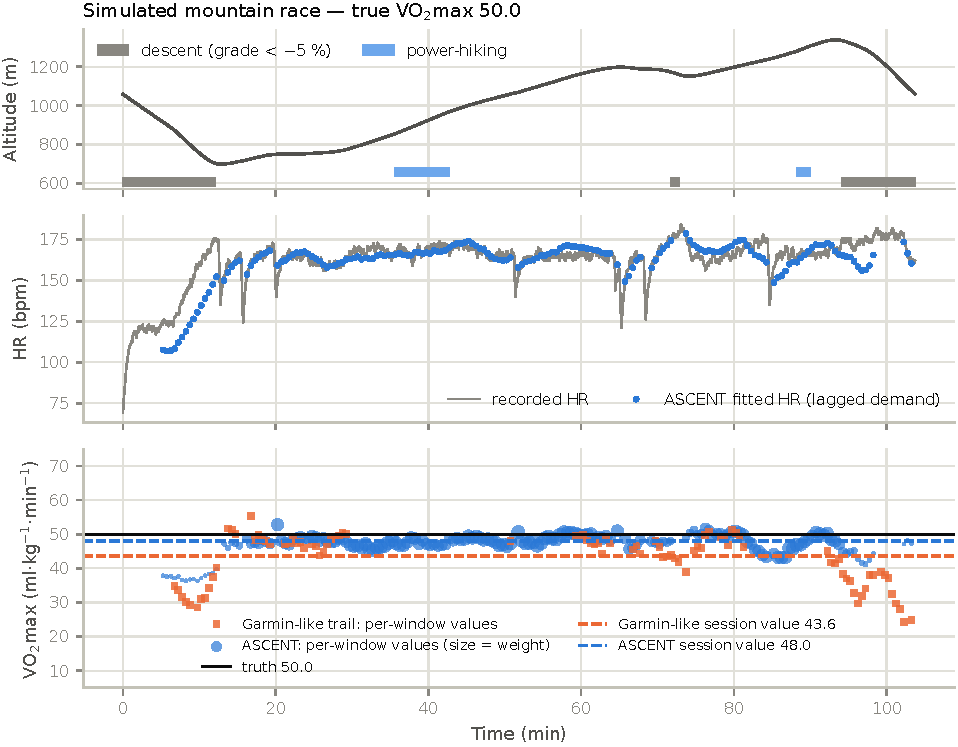
\includegraphics[width=\linewidth]{figures/fig_example_session.pdf}
\caption{A simulated mountain race (true \VOmax{} 50). Top: profile with descents and power-hiking. Middle: recorded HR and the HR fitted by \ascent{} from the lagged demand. Bottom: per-window \VOmax{} values of the Garmin-like trail variant and of \ascent{} (marker size proportional to weight), and both session values.}\label{fig:example}
\end{figure}

\subsection{Ablation}\label{sec:abl}
Table~\ref{tab:abl} and Figure~\ref{fig:abl} remove one component of \ascent{} at a time. In the world without unmodelled horizontal cost, the full estimator is the most accurate variant, or within 0.02 \unit{} of the best one, on every course type (RMSE \nablMFullroadflat, \nablMFulltrailrunnable, \nablMFullmountain{} and \nablMFullskyrun{} from flat road to alpine). Every component pays for itself somewhere. Altitude, drift and the descent model matter everywhere; the gait model matters on alpine courses (RMSE \nablMNoGaitskyrun{} without it); kinetics matter on every course type, least on alpine courses. In the full world, removing the HR kinetics \emph{lowers} the RMSE on mountain and alpine courses. This is error cancellation, not an improvement: ignoring the lag biases the estimate upwards (\nablMBNoLagmountain{} on mountain trails in the matched world), and that offsets the negative bias from unmodelled terrain. Estimating $h$ per session (self-calibration) removed most of the bias (\nablBFreeHmountain{} on mountain trails) but inflated the variance (RMSE \nablFreeHmountain{} vs.\ \nablFullmountain). We therefore keep $h$ fixed at its prior mean.

\begin{figure}[!htbp]\centering
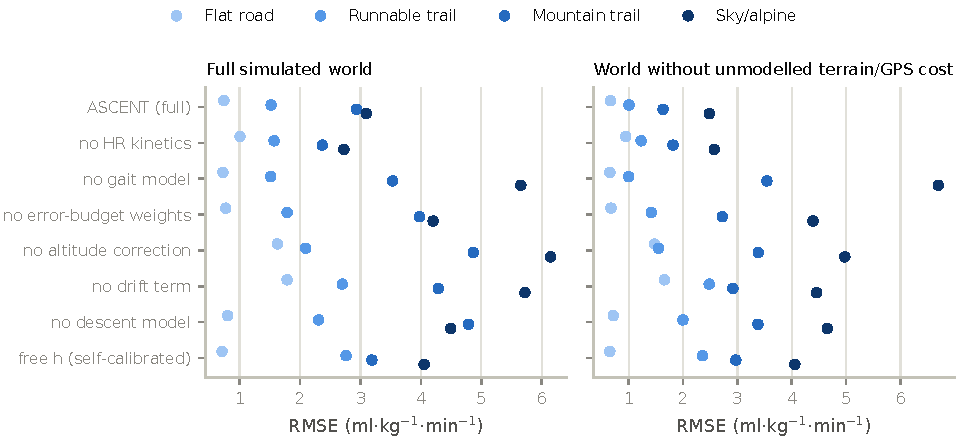
\includegraphics[width=\linewidth]{figures/fig_ablation.pdf}
\caption{RMSE of \ascent{} with one component removed, in the full simulated world (left) and in a world without unmodelled terrain and GPS cost (right).}\label{fig:abl}
\end{figure}

\begin{table}[!htbp]\centering\scriptsize
\caption{Ablation of \ascent: bias and RMSE (\unit), 150 runners, training and race sessions pooled.}\label{tab:abl}
\begin{tabular}{lrrrrrrrr}
\toprule
 & \multicolumn{2}{c}{Flat road} & \multicolumn{2}{c}{Runnable trail} & \multicolumn{2}{c}{Mountain trail} & \multicolumn{2}{c}{Sky/alpine} \\
\cmidrule(lr){2-3} \cmidrule(lr){4-5} \cmidrule(lr){6-7} \cmidrule(lr){8-9}
Variant & bias & RMSE & bias & RMSE & bias & RMSE & bias & RMSE \\
\midrule
\multicolumn{9}{l}{\emph{Full simulated world}} \\
ASCENT (full) & $-$0.3 & 0.74 & $-$0.6 & 1.52 & $-$2.0 & 2.93 & $-$1.4 & 3.10 \\
no HR kinetics & +0.2 & 1.01 & +0.1 & 1.57 & $-$1.2 & 2.37 & $-$0.7 & 2.73 \\
no gait model & $-$0.3 & 0.72 & $-$0.5 & 1.51 & $-$0.5 & 3.53 & +3.4 & 5.65 \\
no error-budget weights & $-$0.3 & 0.77 & $-$0.7 & 1.79 & $-$2.8 & 3.98 & +0.4 & 4.20 \\
no altitude correction & $-$1.5 & 1.62 & $-$1.5 & 2.09 & $-$4.4 & 4.87 & $-$5.6 & 6.15 \\
no drift term & $-$1.6 & 1.78 & $-$2.4 & 2.70 & $-$4.0 & 4.29 & $-$5.1 & 5.72 \\
no descent model & $-$0.4 & 0.80 & $-$1.3 & 2.31 & $-$3.4 & 4.79 & +2.4 & 4.49 \\
free h (self-calibrated) & $-$0.3 & 0.71 & +0.0 & 2.76 & $-$0.2 & 3.19 & $-$0.5 & 4.05 \\
\addlinespace[3pt]
\multicolumn{9}{l}{\emph{World without unmodelled terrain/GPS cost (terrain and GPS shortening switched off, $h$ prior centred at 1)}} \\
ASCENT (full) & $-$0.1 & 0.66 & $-$0.2 & 1.00 & $-$0.4 & 1.63 & +0.0 & 2.48 \\
no HR kinetics & +0.3 & 0.94 & +0.3 & 1.23 & +0.5 & 1.81 & +0.6 & 2.57 \\
no gait model & $-$0.1 & 0.65 & $-$0.2 & 1.00 & +1.7 & 3.54 & +5.2 & 6.70 \\
no error-budget weights & $-$0.2 & 0.67 & $-$0.4 & 1.42 & $-$0.9 & 2.72 & +1.4 & 4.39 \\
no altitude correction & $-$1.3 & 1.48 & $-$1.2 & 1.55 & $-$2.8 & 3.38 & $-$4.3 & 4.98 \\
no drift term & $-$1.4 & 1.66 & $-$2.2 & 2.48 & $-$2.4 & 2.92 & $-$3.6 & 4.46 \\
no descent model & $-$0.3 & 0.72 & $-$1.1 & 2.00 & $-$1.7 & 3.38 & +3.5 & 4.65 \\
free h (self-calibrated) & $-$0.1 & 0.65 & +0.5 & 2.36 & +0.0 & 2.97 & +0.1 & 4.06 \\
\addlinespace[3pt]
\bottomrule
\end{tabular}
\end{table}

\subsection{Sensitivity}\label{sec:sens}
Figure~\ref{fig:sens} varies nine world parameters on mountain-trail sessions. Excluding terrain roughness and the \HRmax{} setting, \ascent's mean bias stays between \nsensMinASCENT{} and \nsensMaxASCENT{} \unit{} across all levels, and that of the Garmin-like trail variant between \nsensMinGtrail{} and \nsensMaxGtrail.

The trail and classic variants are most sensitive to the HR excess on descents (a range of \nrangeGtrailecclambda{} \unit{} for the trail variant) and to drift (\nrangeGtraildrift). The HR-calibrated GAP variant is about as robust as \ascent{} on most parameters, and less biased when the descent excess or drift is weak. Its bias, however, grows with both (ranges \nrangeGtrailhrgapecclambda{} and \nrangeGtrailhrgapdrift), whereas \ascent{} changes little (\nrangeASCENTecclambda{} and \nrangeASCENTdrift). \ascent{} is more sensitive than the Garmin-like variants to hiking economy (\nrangeASCENTwalkecon{} vs.\ \nrangeGtrailwalkecon), because it uses hiking windows.

\ascent's weak spot is terrain roughness. Doubling it moves the bias to \nsensASCENTterrainscaleH, because the fixed prior $h$ no longer matches. All methods depend on the user's \HRmax{} setting: an \HRmax{} set 10 bpm too low shifts the estimates by \nshiftHrmaxLowASCENT{} (\ascent) and \nshiftHrmaxLowGtrail{} (Garmin-like trail). \HRrest{} errors of $\pm5$ bpm matter less (a range of \nrangeASCENThrresterr{} for \ascent).

\begin{figure}[!htbp]\centering
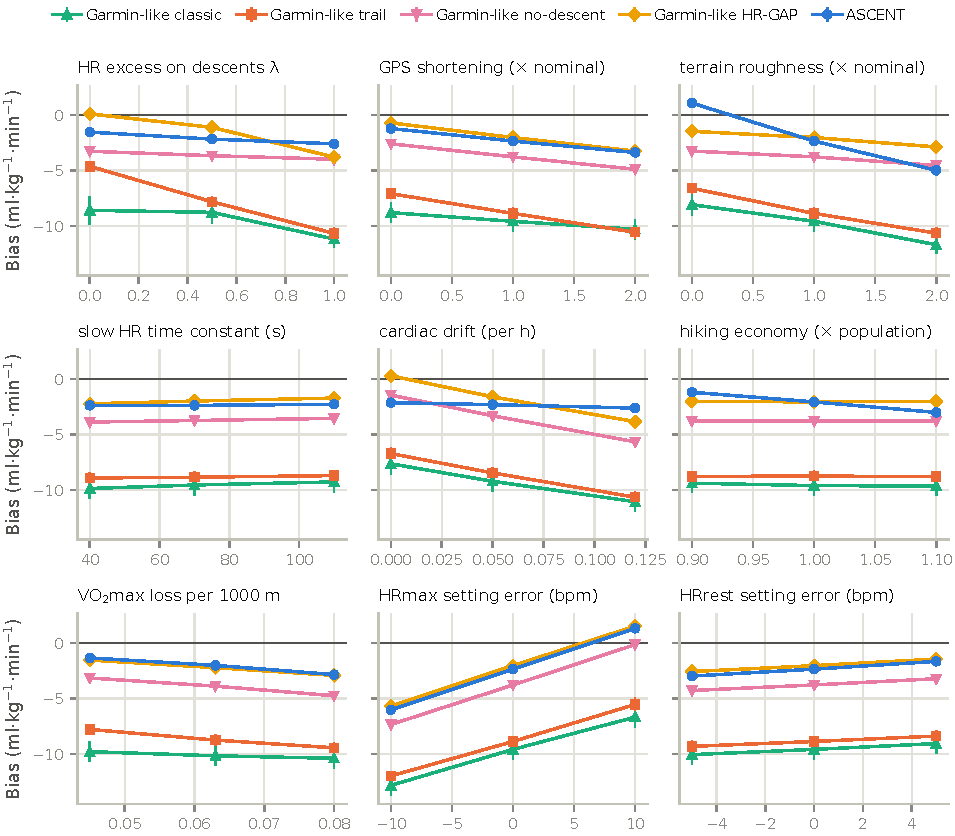
\includegraphics[width=\linewidth]{figures/fig_sensitivity.pdf}
\caption{Bias on mountain-trail sessions (training and race) when one world parameter is varied (mean and 95\,\% CI over 80 runners per level).}\label{fig:sens}
\end{figure}


\section{Reproducibility}\label{app:code}
The accompanying archive contains:
\begin{itemize}[leftmargin=*]
\item the Python package \texttt{ascent}: \texttt{physiology.py} (cost models), \texttt{simulate.py} (data-generating model), \texttt{estimators.py} (Garmin-like reconstructions, \ascent, trackers), \texttt{io.py} (readers for FIT, TCX, GPX and Strava-stream files) and \texttt{cli.py}, a command-line tool that analyses exported activities and keeps a race-aware tracked value across sessions, for example
\begin{center}\footnotesize\verb|python3 -m ascent.cli activity.fit --hr-rest <bpm> --hr-max <bpm> --history log.csv|\end{center}
\item the scripts in the folder \texttt{experiments}, which produce the numbers, tables and figures: \texttt{run\_sim.py}, \texttt{attribution.py}, \texttt{figures.py} and \texttt{make\_tables.py}; the last one writes the \LaTeX{} tables and the macros that hold most numbers quoted in the text;
\item the v2 development: \texttt{fitrec\_v2.py} (candidates on the development half, frozen candidate on the test half), and \texttt{sim\_v2.py} (simulation replay); \texttt{ascent\_v2()} in \texttt{estimators.py} is the frozen v2, and the command-line tool uses it by default (\texttt{-{}-v1} for the original);
\item the FitRec pipeline: \texttt{tools/filtrar\_fitrec.py} extracts the running workouts from \texttt{endomondoHR.json.gz} (downloaded from the FitRec page); \texttt{ascent/fitrec.py} loads the extract; the \texttt{fitrec\_*.py} scripts in \texttt{experiments} (describe, run, analysis, diag, figures) produce Section~\ref{sec:fitrec}. The data themselves are not redistributed;
\item the frozen \ascent{} configuration (\path{results/frozen_ascent_config.json}) and unit tests (\texttt{tests/}).
\end{itemize}
Seeds are fixed. All simulation experiments together take about half an hour on two CPU cores.

\end{document}
